\documentclass[10pt]{article}
% \usepackage[margin=1in]{geometry}
% \newcommand\hmmax{0}
% \newcommand\bmmax{0}
% % % Fonts% %
% \usepackage{luatexja}

\usepackage[T1]{fontenc}
   % \usepackage{textcomp}
   % \usepackage{newtxtext}
   % \renewcommand\rmdefault{Pym} %\usepackage{mathptmx} %\usepackage{times}
\usepackage[complete, subscriptcorrection, slantedGreek, mtpfrak, mtpbb, mtpcal]{mtpro2}
   \usepackage{bm}% Access to bold math symbols
   % \usepackage[onlytext]{MinionPro}
   \usepackage[no-math]{fontspec}
   \defaultfontfeatures{Ligatures=TeX,Numbers={Proportional}}
   \newfontfeature{Microtype}{protrusion=default;expansion=default;}
   \setmainfont[Ligatures=TeX,BoldFont={*-Semibold}]{Source Serif Pro}
   \setsansfont[Microtype,Scale=MatchLowercase,Ligatures=TeX,BoldFont={*-Semibold}]{Source Sans Pro}
   \setmonofont[Scale=0.8]{Atlas Typewriter}
   % \usepackage{selnolig}% For suppressing certain typographic ligatures automatically
% % % % % % %
\usepackage{amsthm}         % (in part) For the defined environments
\usepackage{mathtools}      % Improves  on amsmaths/mtpro2
\usepackage{xfrac}

% % % The bibliography % % %
\usepackage[backend=biber,
  style=authoryear-comp,
  bibstyle=authoryear,
  citestyle=authoryear-comp,
  uniquename=false,
  % allinit,
  % giveninits=true,
  backref=false,
  hyperref=true,
  url=false,
  isbn=false,
  useprefix=true,
  ]{biblatex}
\DeclareFieldFormat{postnote}{#1}
\DeclareFieldFormat{multipostnote}{#1}
% \setlength\bibitemsep{1.5\itemsep}
\newcommand{\noopsort}[1]{}
\addbibresource{Thesis.bib}

% % % % % % % % % % % % % % %

\usepackage[inline]{enumitem}
\setlist[enumerate]{noitemsep}
\setlist[description]{style=unboxed,leftmargin=\parindent,labelindent=\parindent,font=\normalfont\space}
\setlist[itemize]{noitemsep}

% % % Misc packages % % %
\usepackage{setspace}
% \usepackage{refcheck} % Can be used for checking references
% \usepackage{lineno}   % For line numbers
% \usepackage{hyphenat} % For \hyp{} hyphenation command, and general hyphenation stuff

% % % % % % % % % % % % %

% % % Red Math % % %
\usepackage[usenames, dvipsnames]{xcolor}
% \usepackage{everysel}
% \EverySelectfont{\color{black}}
% \everymath{\color{red}}
% \everydisplay{\color{black}}
\definecolor{fuchsia}{HTML}{FE4164}%Neon Fuchsia %{F535AA}%Neon Pink
% % % % % % % % % %

\usepackage[export]{adjustbox}
\usepackage{subcaption}

% \usepackage{pifont}
% \newcommand{\hand}{\ding{43}}
\usepackage{array}


\usepackage{multirow}
% \usepackage{adjustbox}

\usepackage{titlesec}

\usepackage{multicol}

\setcounter{secnumdepth}{4}
\setcounter{tocdepth}{4}

\usepackage{tikz}
\usetikzlibrary{bending,arrows,positioning,calc}
\usetikzlibrary{arrows.meta}
\usetikzlibrary{patterns}
\usetikzlibrary{fadings}
\usepackage{tikz-qtree} %for simple tree syntax
% \usepgflibrary{arrows} %for arrow endings
% \usetikzlibrary{positioning,shapes.multipart} %for structured nodes
\usetikzlibrary{tikzmark}
\usetikzlibrary{patterns}

\usepackage{graphicx} % for images (png/jpeg etc.)
\usepackage{caption} % for \caption* command

\usepackage{tabularx}

\usepackage{bussalt}

\usepackage{Oblique} % Custom package for oblique commands
\usepackage{CustomTheorems}
\usepackage{FuturePromisedEvents}

% \usepackage{svg}
% \usepackage[off]{svg-extract}
% \svgsetup{clean=true}

\usepackage{dashrule}

\newcommand{\hozline}[0]{%
  \noindent\hdashrule[0.5ex][c]{\textwidth}{.1pt}{}
  %\vspace{-10pt}
  % \noindent\rule{\textwidth}{.1pt}
}

\newcommand{\nf}[1]{#1\ensuremath{^{{*}}}}

\newcommand{\hozlinedash}[0]{%
  \noindent\hdashrule[0.5ex][c]{\textwidth}{.1pt}{2.5pt}
  %\vspace{-10pt}
}

\usepackage{contour}
% \usepackage{pdfrender}

\usepackage{extarrows}

% % % My commands % % %

% % % % % % % % % % % %

\usepackage{xskak} % For chess diagram


\usepackage[hidelinks,breaklinks]{hyperref}

\title{Only take me as far as I can go by myself}
% \subtitle{\dots and you don't need me to tell you}
\author{Ben Sparkes}
% \date{ }


\begin{document}

\tableofcontents

\newpage

\maketitle

\section{Introduction}
\label{sec:introduction-1}


{
  \color{red}
  Topic is claims of ability.
  Specifically, ability to reason from some premises to a conclusion.
  Argue that these show an intuitive claim is false\dots
}

Argue against:
\begin{itemize}
\item\label{denied-claim} \emph{An agent may appeal to reasons in support of a conclusion only if the agent used those reasons in some reasoning that yielded the conclusion.}
\end{itemize}

{
  \color{red}
  This is false because the agent draws what would be achieved by witnessing their ability.
}

{
  \color{red}
  Ability statements aren't too interesting for ideal agents.
  However, for bounded agents like us, resources.
  Cost is not reasoning, but reasoning performed.
}

Contraposition seems clear.
If agent used reasons in reasoning, then they may appeal to those reasons in support of the conclusion.
May be challenged and so on, but here interested in when the agent is forming the conclusion.
Unless give a strong normative reading of may, there doesn't seem any way to object.
Would deny that the reasoning is any good, not that the agent can cite their own reasoning.

Instead, contrast \emph{may} with \emph{must}.

Perhaps constitutive of reasoning, but then talk of raesoning instead.

Sketch argument for the conditional.

\begin{enumerate}
\item\label{opp:sketch:1} If conditional is false, then it is possible there are cases in which an agent is unaware of how the conclusion is supported by favoured reasons.
\item\label{opp:sketch:2} If agent is unaware of how a conclusion is supported by reasons, then conclusion may not be supported by those reasons.
\item\label{opp:sketch:3} If conclusion may not be supported, then the conclusion is not supported (from the agent's perspective).
\end{enumerate}

So, the agent may do as they please, but they will fail to establish support, the appeal would be in name only.\nolinebreak
\footnote{
  Alternative sketch:
  \begin{itemize}
  \item Agent to hold \(A\) on the basis of \(R\) requires \(R\) to do some explanatory work.
  \item If agent does not directly respond to \(R\) then \(R\) does not do any explanatory work.
  \item Therefore, reason only if directly respond.
  \end{itemize}
}

Contraposing and re-expressing, the last proposition, reads:

\begin{itemize}
\item If conclusion is supported by reasons, then it is a fact that the conclusion is supported by reasons.
\end{itemize}

Variation on a familiar thought that reasons are factive.\nolinebreak
\footnote{
  For example, \textcite[673]{Cunningham:2020aa}, summarising \textcite{Hornsby:2007aa,Hornsby:2007ab,Hornsby:2008aa} defends:
  \begin{quote}
    Necessarily, if S \(\phi\)'s because p then S knows that p
  \end{quote}
  Where the `because' is a rationalising `because'.
  If \emph{S} knows that \emph{p}, it is a fact that \emph{p}.
}
Here, relation of support is factive.

I think the last premise is more-or-less true, depending on how `may' is understood.
Perhaps the agent does not \emph{know} that the conclusion follows from the premises, but is \emph{confident} that the conclusion follows from the premises --- it would be bizarre if were not a fact that the conclusion is not supported by the premises.
Even so, it seems intuitive that an agent could not have the appropriate confidence without being away of how the conclusion is supported by the premises, and so some variation of \ref{opp:sketch:2} holds.
It seems plausible at least some variation of \ref{opp:sketch:1}--\ref{opp:sketch:3} is sound.\nolinebreak
\footnote{
  Alternative may be to argue for representationalism, or dispositionalism.
  \citeauthor{Neta:2019aa} for example of how these would go.
  Broad, and don't seem quite as informative.
}

I do not think some variation of \ref{opp:sketch:2} holds.
I think an agent may be unaware of how a conclusion is supported by reasons while the conclusion is supported by those reasons (from the agent's perspective and so on).

Focus is on a particular type of ability claim.
For example:
\begin{itemize}
\item ???
\end{itemize}

Argue for reading this as providing an agent with a \emph{license} to appeal to the reasoning (or reasons) that the agent is able to do.

Licenses recast a problem raised by \citeauthor{Davidson:2001aa}:
When we look to explain why an agent performed an act (here, adopting a conclusion), we find there are various account that \emph{could} explain.
(\citeauthor[7--8]{Davidson:2001aa})
\begin{quote}
  But then something essential has certainly been left out, for a person can have a reason for an action, and perform the action, and yet this reason not be the reason why they did it.
  Central to the relation between a reason and an action it explains is the idea that the agent performed the action \emph{because} they had the reason.\nolinebreak
  \mbox{}\hfill\mbox{(\citeyear[9]{Davidson:2001aa})}
\end{quote}
As \citeauthor{Hieronymi:2011aa} expresses, we seek `an explanation which shows, not merely what, from another’s point of view, \emph{could} count in favour of acting, but why that person did, in fact, act' (\citeyear[417]{Hieronymi:2011aa}).

Following \citeauthor{Davidson:2001aa}, then, reasons or reasoning only explain an action provided there is a causal relation between the reasons the agent had or the reasoning the agent performed, and the action.\nolinebreak
\footnote{
  Note on the inclusion of reasoning here.
  Later \citeauthor{Davidson:2001aa}: `I do not see how the right sort of causal process can be distinguished without, among other things, giving an account of how a decision is reached\dots' (\citeyear[232]{Davidson:2001aa}), etc.
  And, my focus.
}
If this is sound, then the difference between what \emph{could} explain and what \emph{does} explain is only a matter of what happened --- a causal relation does not distinguish explanation from non-explanation, but actual explanation from potential explanation.\nolinebreak
\footnote{
  In \citeauthor{Hieronymi:2011aa}'s phrasing: Without a causal relation we get an answer to ‘from so-and-so’s point of view, why do so such and such?’ rather than ‘why did so-and-so do such-and-such?’ (\citeyear[417]{Hieronymi:2011aa}).
}\(^{,}\)\nolinebreak
\footnote{
  {
    \color{red}
    This is different to the relationship that \citeauthor{Neta:2019aa} notes between reasons why and reasons for which.
    In short, reasons why are not always reasons for which, because there are explanatory relations which are in a sense `structural' and therefore are not seen as reasons from the agent's point of view.
    So, I'm colourblind, but that is not a reason for which I believe the two different colours are the same colour, though it explains why.
    Rather, the reasons for which is that both objects appear the same colour to me.

    The distinction I am interested in can be seen as distinction between the way a reason \emph{which} may support an attitude.
  }
}

Even if causal relations to not resolve the problem of distinguishing what could explain from what does explain, I take this problem to be genuine.
There is often no unique explanation for an action, potential explanations \emph{do} explain, but (merely) potential explanations do not explain what actually happened.
Yet, if potential explanations do explain, and an agent has a guarantee that a potential explanation obtains, then the agent has the guarantee of an explanation.

\begin{note}[Neta on Davidson/Anscombe]
  \citeauthor{Neta:2019aa} reconstructs this in terms of explanatory reasons in response to Anscombian `Why' questions.
\end{note}

% One does not need the theoretical backing to observe that the integer expression of \(7^{3}\) may be obtained by either mental arithmetic or a calculator.
% And that if one is confident in their ability to perform mental arithmetic, then the use of the calculator demonstrates what they would obtain by performing the reasoning.
% So, if one is provided with the information that one has the ability to perform the mental arithmetic to see that \(7^{3} = 343\), or that the calculator will show \(343\) after typing \(7^{3}\) in and hitting enter, it seems that either of these potential explanations may be cited as the explanation for holding that \(7^{3}\) is \(343\).

% What explains why I hold that \(7^{3}\) is \(343\) is that the calculator would demonstrate that it is so, or \dots is that I have the ability to demonstrate that it is so.
% The information provides only states that \(7^{3} = 343\) is the result of some process, and so I take that process to support holding that \(7^{3} = 343\).

{
  \color{red}
  The \citeauthor{Davidson:1963aa} motivation is quite general.
  I end up focusing on a particular case, where there are additional constraints to draw on.
  However, the result is of this kind, and I take this to be partial motivation for the possibility of these cases even when the additional constraints do not apply.

  Even so, role of ability in reasoning is interesting, and an instance of this type of thing.
}


\begin{note}[Fine distinction]
  The fine distinction is between an agent responding to reasons and an agent's action being supported by reasons.
  {
    \color{red}
    \emph{This!!!}
  }
  It is important to distinguish between the state of the board and the rules of chess, which are sufficient to derive the particular reasons, from this specific reason for which the move is possible.
  That it is a knight, knights can move, etc.
\end{note}

\begin{note}[Rationality]
  Another way to look at this is in terms of a distinction between kinds of irrationality.
  Admittedly, claims to rationality are strong.
  So, distinguish between the failure to respond to reasons, and the absence of reasons to respond to.
\end{note}

\hozlinedash

That an agent is able to reason may not be necessary, but helps with the explanation being potential --- a helpful divide between potential explanations and hypothetical explanations, perhaps.
Sufficient, at least.
Necessary and sufficient conditions aren't of interest.


Causal relations may not be correct.
Well, seems must not be correct.
This only goes part of the way.

Potential seems redundant.
Section ???

Here, agent obtains a license to a potential explanation.
Information about ability provides the agent with the information that the explanation could hold explain, or could stand in the appropriate causal relation.
Hence the agent performs the action `because' of the reasons or reasoning that would be invoked in the potential explanation.

{
\color{red} This skips over some details, esp.\ about how reasons/potential explanations are under-specified.
}

If the thing licensed isn't a potential explainer, then the agent would not have the ability, etc.\

Problem tasked with as theoreticians --- identifying the explanation --- is, in a sense, exploited by the agent given certain conditions.

Straightforward incompataibility.
Yes.
But only if assume (or demand) that the causal explanation is complete\dots

{
  \color{red}
  First part of the paper is walking through this carefully.
}
The upshot of denying~\ref{denied-claim} is flexibility in understanding agency.
Isolating, illustrating.



An important feature is that in the cases of interest, the conclusion does depend on reasoning to be true.
Some cases fail.
For example, agent cannot conclude that they have reasoned to the conclusion.
As, it is only the case that the agent has reasoned to the conclusion if the agent has performed the reasoning.
Reflexive content is often a source of trouble, but here the problem is more mundane.
An agent cannot turn on a light by reflecting on their ability, the agent must flick the switch in order for the light to turn on --- and reflexively referencing one's own reasoning requires a similar witnessing event.

Reasoning is great for various things other than obtaining a conclusion.
Agent goes with licensed reasons, they do not get this stuff.
However, the agent does get other things.

\subsection{Overview}
\label{sec:overview}

This section has set out the general goal.
It is quite broad.
The argument is quite focused.

Three sections that follow.
\begin{enumerate}
\item General argument, issues, etc.
\item Specifics of failure.
\item Potential for potential.
\end{enumerate}
This includes two passes for both arguments.
First in the general outline, and again in the specifics.

This involves some redundancy.
However, this permits details where they matter.
Primary upshot of this compromise is that the first section will be sufficient for the big picture.
Also, isolated conclusions.
Second section provides results about expansion of ability.
Third section provides results about how to understand a plausible reasoning pattern.


\hozlinedash

\section{Potential strategies}
\label{sec:potential-strategies}

\begin{note}[Narrowing cases]
  The motivating idea behind licensing is broad.
  It applies to any situation in which an agent is confident that a potential explanation is available.

  However, the argument for licensing is narrow.
  Look to specific cases.

  In the same way that there may be multiple potential explanations available to the agent, there may be multiple accounts to us as theorists.

  If an account can be given that does not involve licensing (or that do not involve the idea of licensing as anything other than a mistake), then the test is whether licensing is a best account.

  Assume that an account can be given that does not involve licensing.
  I doubt that it is possible to show that any given account is necessary.
  However, whether or not an account is best is not determined by the particular case.
  Depends also on the role of the account in other cases.
  Secure licensing in particular cases provides some support over alternatives when there is competition.\nolinebreak
  \footnote{
    Maybe a note here about the principle of charity.
    This is, I think, also a Davidsonian idea.
    Charity in the sense that one assumes that there is a rationalisation --- a (complete) explanation --- available.

    Charity, assume that if an agent's action is the result of reasoning then it may be rationalised --- in the sense of providing a complete explanation.
    Even a poor, but complete, explanation is preferable to an incomplete explanation (and hence absence of rationalisation).

    % May motivate with ideal cases.
    % Ideal cases seem to include possession of an explanation.
    % Soften the ideal by relaxing standards governing the quality of the explanation, rather than the existence of an explanation.
    % A poor explanation remains an explanation; potential explanation is only a \emph{potential} explanation.

  Corollary is the denial of this ordering on explanations.
  Sometimes appeal to a potential/incomplete explanation is better than a complete explanation.

  Conflicts with charity only if explanation is understood as complete explanation.
  Hence, I do not think that this conflicts with the spirit of charity, though it may conflict with particular accounts of charity.
  }

  This is about theory of explanations/reasons/reasoning.

  This limits attention.
  May be that licensing is rarely a best account.
  However, so long as it is a contender, then the main goal has been achieved.
\end{note}

\begin{note}[Outline of section]
  The goal of this section is to isolate a particular pattern of reasoning:
  \begin{enumerate}
  \item Information that agent possesses ability to reason \(\phi\).
  \item Endorsement of ability (not simply testimony).
  \item `Factive' inference to \(\phi\) being the case.
  \end{enumerate}
  Key piece of this reasoning is:
  \begin{itemize}
  \item Agent has the ability to \(\alpha\phi\) only if \(\phi\) is the case, where \(\alpha\) is some factive thing.
  \end{itemize}
  This is a necessary condition on the agent possessing the ability.
  Therefore, \emph{that} the agent possesses the ability can not be used to support \emph{that} \(\phi\) is the case.
  For the agent must already implicitly assume that \(\phi\) is the case.

  That the agent is informed is straightforward.
  The agent may avoid endorsing the ability, but this leads to some unnatural/indirect inference regarding assertion.
  Hence, endorsement of ability seems a plausible line of reasoning.

  Restructuring, I need to file some problems with ability inferences prior to working through testimony.

  In short, the problem is that there is no certainty with ability when the proposition is novel.
  For, the ability concerns a particular event type, bounded to the agent's current state.
  And as the agent has not yet witnessed their ability, at most one can obtain a high degree of confidence.
\end{note}

Consider the following:
\begin{enumerate}
\item\label{chess:claim:1}\label{chess:claim:1:conditional} If you are able to reason with the rules of chess, then you have the ability to reason from the game state (described in figure~\ref{fig:chess:board}) to the proposition that White cannot prevent Black from occupying c4 on their (Black's) second move.
\end{enumerate}

I assume claim~\ref{chess:claim:1} is true, but not immediately obvious.
And, in particular, that some reasoning from the rules of chess and the game state is required to verify the truth of the highlighted proposition.

For, in order to show that White cannot prevent Black from occupying c4 on their second move, you need to consider the moves that would be possible for Black on their second turn given the move that White made on their first turn in response to the move that Black made on their first turn, and so on.


\begin{figure}[h]
  \centering
  \mbox{ }
  \hfill
  \begin{subfigure}{.4\textwidth}
    \begin{adjustbox}{minipage=\linewidth,scale=0.7}
      \centering
      \newchessgame[
      setwhite={ka5,pa3,pb4,pc4,pe5,pf6,bg5,bh5}, %{rc1,kh1,pa2,pb2,ph2,pf6,pg6,nc7,qf7},
      addblack={pa6,pb7,pc6,pe6,pf7,kc7,nd7,nd4}, %{rg2,pb5,pe5,qd6,pa7,pb7,ra8,bc8,kd8,bf8},
      ]%
      \setchessboard{showmover=false}%
      \chessboard
    \end{adjustbox}
    \caption{
      Game state\newline
      \mbox{ }\newline
    }
    \label{fig:chess:board}
  \end{subfigure}
  \mbox{ }
  \hfill
  \mbox{ }
  \begin{subfigure}{.4\textwidth}
    \begin{adjustbox}{minipage=\linewidth,scale=0.7}
      \centering
      \newchessgame[
      setwhite={ka5,pa3,pb4,pc4,pe5,pf6,bg5,bh5}, %{rc1,kh1,pa2,pb2,ph2,pf6,pg6,nc7,qf7},
      addblack={pa6,pb7,pc6,pe6,pf7,kc7,nd7,nd4}, %{rg2,pb5,pe5,qd6,pa7,pb7,ra8,bc8,kd8,bf8},
      ]%
      \setchessboard{showmover=false}%
      \chessboard[
      arrow=latex,
      linewidth=1pt,
      shortenstart=.8ex,
      shortenend=.5ex,
      pgfstyle=straightmove,
      strokeopacity=0.4,
      fillopacity=0.4,
      color=black,
      pgfstyle=border,
      markfields={c4,a3,a5,g6,c5},
      % markmoves={b7-b6,c6-c5,d4-c2,d4-b5,d4-f5,d4-e2,d4-f3,d4-b3,d7-c5,d7-b6,d7-b8,d7-f8,d7-f6,d7-e5,d7-e5,c7-c8,c7-b8,c7-d8,c7-b6,c7-d6}%{f7-g8,f7-e6,f7-d5,f7-c4,f7-b3,f7-e8,c7-d5,c7-b5,c7-a8,c7-e8,g6-g7,a2-a3,b2-b3,c1-a1,c1-b1,c1-d1,c1-e1,c1-f1,c1-g1,h2-h3,h1-g1,c1-c2,c1-c3,c1-c4,c1-c5,c1-c6}
      ]
    \end{adjustbox}
    \caption{Example fields White cannot prevent Black from occupying after two moves.}
    \label{fig:chess:move}
  \end{subfigure}
  \hfill
  \mbox{ }
  \caption{Black to checkmate in four moves.\protect\footnotemark}
  \label{fig:chess}
\end{figure}
\footnotetext{
  Puzzle 150 of \citeauthor{Emms:2000aa} (\citeyear[33]{Emms:2000aa}).
  \citeauthor{Emms:2000aa} provides the following solution:
  \begin{quote}
    \variation{1... Nb6!}
    (threatening \variation{2... Nb3\#})
    \variation{2. b5}
    (or \variation{2. Bd1 Nxc4+} \variation{3. Ka4 b5\#})
    \variation{2... c5!}
    \variation{3. bxa6 Nxc4+}
    \variation{4. Ka4 b5\#}
    \textbf{(0-1)}\nolinebreak
    \mbox{}
    \hfill
    (\citeyear[46]{Emms:2000aa})
  \end{quote}
}

To illustrate, Black may move the pawn from b7 to b5 on their first turn, and so be in a position to capture White's pawn on c4 in their second turn.
However, White may then prevent Black from occupying c4 on their next turn by using their pawn on c4 to capture Black's pawn on b5.
So, Black moving their pawn from b7 to b5 on their first turn is not an initial move of interest.

Still, there are only (a little more than) a handful of alternative moves and countermoves to consider, and so I not only assume that claim~\ref{chess:claim:1} is true, but I also assume that you also hold claim~\ref{chess:claim:1} to be true.

\begin{note}[Some motivation for holding claim 1 to be true]
  Perhaps you have an effective method for identifying a strategy for Black.
  Perhaps you are able to exhaust all the strategies available to Black and identify those which ensure c5 is occupied on Black's second move.
  Perhaps you have solved a sufficient number of sufficiently challenging chess puzzles.

  Or, you solved a lot of chess problems.

  Whichever way, general ability.
\end{note}

Precisely, I assume that you hold claim~\ref{chess:claim:1} to be true at some interval between the point at which I claimed~\ref{chess:claim:1} is true and the present time or the point at which you demonstrated claim~\ref{chess:claim:1} to be true.\nolinebreak
\footnote{
  If a fresh instance of claim~\ref{chess:claim:1} is desired, one may substitute (e.g.) `a3', `a5', `g6', or `c5' for `c4'.
}
For ease of exposition, I will adopt the perspective of some point in that interval.

\begin{note}[Reasoning sketch]
  With the above, sketch out simple reasoning.
 {
   \color{red}
   \begin{enumerate}
   \item\label{simple:conditional:claim} If I have a moderate ability to reason with the rules of chess, then I have the ability to reason from the game state (described in figure~\ref{fig:chess:board}) to the proposition that White cannot prevent Black from occupying c4 on their second move.
   \item\label{simple:conditional:antecedent} I have a moderate ability to reason with the rules of chess.
   \item\label{simple:conditional:consequent} I have the ability to reason from the game state to the proposition that White cannot prevent Black from occupying c4 on their second move.
   \item\label{simple:conditional:factive-demonstration} It is not possible to demonstrate something that is false.
   \item\label{simple:conditional:necessity} If it is not the case that White cannot prevent Black from occupying c4 on their second move then \ref{simple:consequent} is false.
   \item\label{simple:conditional:focus} White cannot prevent Black from occupying c4 on their second move.
   \end{enumerate}
 }
\end{note}

By assumption the agent has not reasoned from the rules of chess and the game state to \ref{simple:conditional:focus}.
In turn, the agent does not hold \ref{simple:conditional:focus} to be true due to a particular strategy that Black can enact.
Instead, \ref{simple:conditional:factive-demonstration} requires that the agent cannot be confident that they have the ability to demonstrate a strategy without being confident that \emph{some} strategy exists.\nolinebreak
\footnote{
  Assumes a factive reading of `demonstrate', this assumption will be held throughout the paper.
  Non-factive counterpart.
  If required, replace `\emph{term}' with `\nf{\emph{term}}' to indicate non-factive reading.
  Hence, `\nf{demonstrate}' is non-factive/appearance of demonstration.
  Likewise, `\nf{see}' is non-factive/appearance of `see'.

  For example, if the agent sees a donkey, then factivity of sight entails existence of donkey, while if the agent \nf{sees} a donkey, the agent may be hallucinating, the object may be a cleverly disguised mule, a hologram, etc.
}
And, it seems, agent's prior confidence of ability meshes with the conditional provided by the informer.
So, as it seems the agent is permitted to be confident that they are able to demonstrate the existence of a strategy, the agent is required to be confident that a strategy exists.

I take the broad outline of this reasoning to be compelling.
Agent's possesses general abilities, agent is not required to understand specifics that follow from general ability, informer's observe specific abilities which follow from general abilities, and once informed agent incorporates this information.

Interest is in how this works when the only information the informer provides is a conditional linking general to specific.
So, not support for the particular fact otherwise.

\begin{note}[Intuition for only conditional information]
Written communication, so I'm not focused on \emph{your} ability, so to speak.
Instead, claim~\ref{chess:claim:1} holds in general, so it is fair to reason that in order for me to make the claim I must have reasoned from the game state to a strategy.
\end{note}

\hozlinedash

\begin{note}[The details matter]
  If the agent is given conditional information, then the details matter.
  For, the fact rests on the reasoning.
  Relation of support tracing from premises to conclusion.
  Here, support as generic.
  Sketch suggests that support works out, but ability suggests two different ideas.
\end{note}

\begin{note}[Two options with ability]
  First, there is the attribution of ability.
  Second, there is witnessing ability.

  This leads to two ways of reading the argument.
\end{note}

\begin{note}[Two ways of reading the argument, 1]
  Two different ways of understanding the argument.
  \begin{enumerate}
  \item Attribution.
  \item Witnessing.
  \end{enumerate}
  Attribution is working form the attribute of having the general ability.
  Witnessing is working from witnessing the ability.

  \begin{multicols}{2}
    Attribution:
    \begin{enumerate}
    \item If general then specific.
    \item Prior support for general
    \item Have the general ability
    \item Have the specific ability
    \item Strategy exists
    \end{enumerate}

    Witness:
    \begin{enumerate}
    \item If general then specific
    \item Prior support for general
    \item General to witness of specific
    \item Provide witness
    \item Strategy exists
    \end{enumerate}
  \end{multicols}

  Witnessing, the agent relies on applying their ability and the potential attribution is unimportant.
  Attribution, the agent relies on the attribution, and the potential reasoning is unimportant.

  The two are related.
  If the agent has the ability, then the agent has the potential to reason.
  And, if the agent is able to apply their ability then the agent has the potential to attribute the general ability to themselves.

  Reasoning is distinct, and potential to make a difference with respect to support.
\end{note}

\begin{note}[Tangential ex. for att. vs. witt.]
  An tangential example may help illustrate the difference.

  Height barrier to a ride.
  Attribute, particular height.
  Witness, walking under the bar.

  Here, arbitrary.
  Depends on the administration.
  Height is key, and the bar is a test.
  Or, bar is key, and height is an approximation.

  Rough around the edges.
  Taller, but slouching.
  Shorter, but hair.

  Preserved under transformations.
\end{note}

\begin{note}[Two ways of reading the argument, 2]
  Analogy does not stretch beyond illustrating basic difference.
  Ride entrance is defined in this way.
  Support is not.
  Still, difference.
  Potential for this to reflect difference in whether support flows.

  The characterisation of attribution and witnessing is rough, and will be detailed in time --- the following paragraphs, and the main argument.

  The latter, witnessing, reflects opening ideas.
  The agent appeals to potential reasons, as the agent hasn't done the reasoning.
  The former does not require this.

  The former is problematic.
\end{note}

\begin{note}[Two ways of reading the argument, 3]
  Worry that this is very much in the weeds, so to speak.
  Yes.
  Limitations from ability and from information.

  Still, significant.
  If witnessing is required in some cases, then question of whether this holds in cases where it is not required.
  And, significant because\dots (no detailed account).
\end{note}

\begin{note}[Quick argument/upshot/stakes]
  Turn this into something of an argument.
  \begin{enumerate}
  \item\label{supp:arg:claim} Claim
  \item\label{supp:arg:need-supp} Would not be reasonable without support.
  \item\label{supp:arg:supp} Hence, if inference is okay then must be provided with support.
  \item So, either some additional support, or the agent rejects the conditional, or reduces confident in antecedent.
  \item\label{supp:arg:reasonable} Reasonable for the agent to hold true, and retain confidence.
  \item Additional support.
  \end{enumerate}

  Above, background reflections provided additional support.
  If not, then the agent would be required either to reject the conditional or lower confidence in ability.

  Inclined to think that [the toy argument from~\ref{supp:arg:claim} to~\ref{supp:arg:supp}] holds most of the time.
  Hence, the interest with \emph{ability} claims.
  Often there is no other route provided, but here there is.

  The interesting thing about ability is that there's no simple characterisation.
  Have the ability to do something, without recognising that one has the ability.
  Yet, this puts the agent in a position to verify.

  Easy to see when given some simple rules.
  For example, mathematics or logic.
  This isn't simply the ability to establish any theorem in the logic case.
  Some proofs may be out of reach.

  A little more straightforwardly by reversing, absence of a witness does not show inability.

  So, agent has information about potential reasons, so to speak.

  Replace with:
  \begin{enumerate}
  \item So, either some additional support, or the agent rejects the conditional, or if ability then licenses support from ability.
  \end{enumerate}

  Focus of the paper is motivating this additional option.
  I haven't yet argued that no parallel to the background reasoning works in all cases.

  The upshot is that this opens up understanding of agents.
  However, argument is somewhat limited in scope.
  Specific cases, therefore open to further constraints.
  The most straightforward is strengthening the antecedent of the conditional, so that it only applies when the agent lacks additional support.

  Still, two options are not exclusive, and I counterpart argument will highlight a handful of cases to demonstrate potential.
  And, note that the focus on ability allows deviations from familiar accounts to be isolated.
  Of course, this limits generalisations, rationality goes beyond responding to reasons.
  However, given the relative uniqueness of ability, many of the arguments in support of general positions will continue to hold, and as such licensing supplements preferred theory.
\end{note}

\begin{note}[No detailed account]
In addition, no detailed account of why you hold claim \ref{chess:claim:focus-prop} is true follows from understanding the rules of chess and the game state alone.
For, one may understand the rules of chess and the game state while lacking the ability to demonstrate that claim~\ref{chess:claim:focus-prop} is true --- understanding the rules of chess and the game board is distinct from the ability to construct strategies.\nolinebreak
\footnote{
  Here I am relying on a principle \emph{like}:
  \begin{itemize}
  \item An agent's grasp of \(\Sigma\) can provide an account of why they hold \(\phi\) is true only if the agent has the ability to demonstrate that \(\phi\) follows from \(\Sigma\).
  \end{itemize}
  {
    \color{red}
    Whether or not this claim is true depends in part of how ability is understood\dots
  }

  Perhaps it is the case that claim~\ref{chess:claim:focus-prop} is sufficiently obvious to guarantee that the agent has the ability.
  Still, the reasoning involved differs only in complexity from the reasoning involved in showing that White cannot prevent Black from checkmating in four moves, and I doubt that this claim is sufficiently obvious.
}
\end{note}

\begin{note}[First part focus]
  First part focuses on conditional and problems with attribution.
  Sketch the problem.
  Then, alternative.
  Details in {\color{red} section ???}.
  
\end{note}

\begin{note}[Attribution outline]
  The focus of {\color{red} section ???} is whether the agent obtains support for the existence of a strategy from their confidence that they have the (general) ability to reason with chess, and the informer's claim that if they have the (general) ability to reason with chess then they have the (specific) ability to demonstrate a particular strategy.

  The primary conclusion of {\color{red} section ???} is that the agent does not obtain support.
  The argument for the primary conclusion of {\color{red} section ???} consists of two premises.

  \begin{itemize}
  \item Novel information provides irresolute support.
  \item Irresolute support is insufficient for factive inference.
  \end{itemize}

  \begin{itemize}
  \item Agent has support for \(A(\psi)\)
  \item \(A(\phi) \rightarrow A(\psi)\) is novel information.
  \item No independent support for \(A(\psi)\).
  \item Without independent support for \(A(\psi)\), the agent's support for \(A(\psi)\) is just the agent's support for \(A(\phi)\).
  \item So, agent's support for \(A(\psi)\) is irresolute.
  \item If irresolute, then no support by factive inference.
  \end{itemize}

  Irresolute.
  Something missing.
  For example, floating in water.
  Easy test.
  Well, salt content.
  So, resolute for some, irresolute for others.

  Depends on the proposition.
  Float in water of the same consistency.
  Sure, trade between degree of support and specificity of proposition.

  Idea is that some price is fixed, irresolute if some debt.
  Resolute if otherwise fine.

  Non-committal terminology.

  Simple gloss in terms of possible worlds is ruling out and making unlikely.
  As novel information, new worlds get added in, and the agent is only in a position to consider these unlikely.

  \hozlinedash

  Possible for the support to hold and the conclusion to be false.
  Contrast, doing the proof.
  If conclusion does not hold, the agent was mistaken about the support provided.

  Doing the reasoning would be conclusive.

  Witness doesn't provide conclusive support either, but different because it is an incomplete argument.
  Potential reasons.

  Defeasible is close, but avoid.
  One the one hand, could turn out false.
  Still, two problems.
  Good arguments of this kind.
  Works quite generally for the type of reasoning and the reasoning itself.

  For sure, defeasible argument seems fine, with conclusion that the agent cannot avoid, etc.
  Factive doesn't follow from this.
\end{note}

\hozlinedash

\begin{note}[Attribution sketch: Novel information]
  {
    \color{red}
    Key point here is that the agent's support for \(A(\psi)\) just is the agent's support for \(A(\phi)\).
    Rather, if the agent has support for \(A(\psi)\) then the support is irresolute.
  }
  General ability with novel information provides irresolute support for (specific) ability.

  Assume that the agent has support for general ability prior to information provided by the informer.
  Made distinction between resolute and irresolute.
  If irresolute for general, then easily irresolute for specific ability.
  If resolute, then this doesn't extend to specific ability.

  {
    \color{red}
    Similar to hardiness of knowledge --- explored in detail further along.
    Just as agent is not free to ignore potential counterevidence, the agent is not free to extend their ability to anything which follows.
  }

  Conditional information.
  If something is the case, then something else is the case.
  So, if the agent has the general ability, then the agent has the specific ability.
  Agent doesn't have any independent support for specific ability.
  Agent's support isn't resolute, because failure would provide agent with a counterexample, etc.

  With information, enriched take on general ability.
  Distinguish these.
  Resolute for ability before information.
  Irresolute for ability after information.
\end{note}

\begin{note}[Attribution sketch, part 2]
  {
    \color{red}
    Key point: Either no support (either kind) for \(A(\psi)\), or commitment to \(\psi\).
  }
  In turn, failure of transmission of support.

  This is because of the factive inference requiring something stronger to be the case than the agent has support for.

  Agent doesn't have independent support for \(\psi\).

  Basically, still possible for \(\psi\) to be false.
  Therefore, support for \(A(\psi)\) is irresolute/limited.
  However, as support for \(A(\psi)\) is irresolute, then the agent isn't in a position to make the factive inference.

  Then, failure of transmission argues that the agent assumes irresolute support?
  Right, that's kind of interesting.
  So, intuitive that the agent doesn't get \(\psi\) by factive inference, but also agent doesn't get irresolute support for \(\psi\).
  For, this is assumed in order to get \(A(\psi)\).

  So, it one grants that the agent gets irresolute support for \(A(\psi)\), this doesn't extend to \(\psi\).
  Hence, the terminology of a commitment.

  So, either no support (either kind) for \(A(\psi)\), or commitment to \(\psi\).
\end{note}

\begin{note}[Attribution transmission failure parallel]
  This can be read into the Dretske examples, given some leeway.
  For, the visual experience lends support to (factive) sight.
  Yet, the resulting factive inference requires the agent to see in order to make the inference.
  However, experience does not grant this.

  So, this gets solved by arguing that the agent does see.
  The move is certainly available --- here, neutrality.
  In contrast, the option is not available here.
  The agent has not performed the inference.
  Second contrast, then, is that it is possible for the agent to do the reasoning.
  In the Dretske example, it's not clear that this is possible.
  Or, so I conjecture.
  It is not clear, if one is not currently seeing, what one could do, at least on par with putting pen to paper.
\end{note}

\begin{note}[Attribution sketch, part 2.5 --- trouble with transmission]
  Failure of transmission means that the agent does not obtain support for \(\psi\) from attributive reasoning.

  So, if support for \(A(\psi)\) then commitment to \(\psi\).
  Hence, either no support for \(A(\psi)\) or commitment to \(\psi\).\nolinebreak
  \footnote{
    Possible for both disjuncts.
    Though, hard to see why the agent would be committed if not for irresolute support.
  }
  And, counterpart proposition to commitment which is irresolutely supported.

  Issue is whether this is satisfactory.
  Tension is intuitive grasp on reasoning contrasted with limited conclusion from attributive reasoning.
  Could restrict the agent.

  Doubt there is any argument to show that the agent must have support.
  Still, seems to be something about understanding of ability.

  \begin{enumerate}
  \item\label{intuition:attitude-to-fact-from-ability-to-demonstrate} If agent is confident that they are able to show something which is true independent of ability, then it seems that agent does not have the option of withholding attitude toward that thing while retaining confidence in ability.
  \end{enumerate}

  Argument shows that this idea is incompatible with reasoning via attribution.

  Problems are about support for \(A(\phi)\) extending.
  Agent's support for \(A(\phi)\) remains the same (roughly, information could have an impact).
  Key issue is that the informer provided new information.
  However, the new information doesn't influence ability itself.

  The problems here arise because of attribute and novel information.
  Limited to type of reasoning.

  Note, this isn't particularly strong.
  It's from the agent's epistemic standpoint.
  It may be that the rules of chess require the fact (this seems likely).
  And, the fact may be sufficiently simple to indicate a failing of general ability (also likely).
  However, the agent does not have the strategy.

  So, support for general ability.
  Don't need the conditional to apply the ability to reach \(\psi\).
  Problem is coming from the having support for ability, rather than execution of ability.

  So, backwards looking, in a sense.
  With the novel information, agent is required to hold that \(\psi\) is the case.
  However, \(\psi\) follows from witnessing ability.
  Limit to commitment clashes with confidence in ability.

  Clash only if there is no alternative.

  Plausibility of~\ref{intuition:attitude-to-fact-from-ability-to-demonstrate} motives interest in witnessing.

  Would put the agent in position of resolute support for \(\psi\).
  However, agent has not done the reasoning.

  Still, novel information doesn't put the agent in a worse position with respect to application of the general ability.
  Novel information, and this shouldn't be taken against \(A(\phi)\).

  If the agent has the general ability, and the information is true, then the agent has the specific ability regardless of informer providing the information that this follows.

  \hozlinedash

  Intuition~\ref{intuition:attitude-to-fact-from-ability-to-demonstrate} is weaker than some nearby relatives.
  If committed and no opposing reason, then confidence.
  Seems strong.
  Perhaps too strong for what I need.

  Familiar to entitlement.
  Here, entitlement doesn't apply.
  However, executing ability does.

  Key difference to sight example, is that there is no need to deny confidence.
  The problem identified is appeal to some collection of reasons.
  Grant the agent license to appeal to these, then confidence seems fine.
  However, if deny this, then reject conditional or withhold consequence.
  {
    \color{red}
    Interest in the latter is this overstepping, but with option.
    Return to some parallels later.\nolinebreak
    \footnote{
      Basically, with the seeing case, the agent possesses the relevant reasons, but is not able to distinguish them.
      This is somewhat close to Pritchard's disjunctivism.
    }
  }

  Maybe in line with the \citeauthor{Harman:1973ww} idea, the novel information doesn't show that the agent doesn't know, but prevents the agent from expanding their prior knowledge.
\end{note}

\begin{note}[Attribution sketch, part 3]
  So, get that the agent is committed to \(\psi\).
  However, this is non-factive.
  Possible to be committed in this sense to a contradiction.
  E.g.\ with a nice case of co-reference.
\end{note}

\begin{note}[Through sketch, summary]
  Grant confidence, but still have problem of the reasons that the agent is appealing to.
  The agent has good support.
  However, the reasons are distinct.
  Further, the agent cannot avoid a consequence of those reasons.

  Note, potential, not hypothetical.
  Place `might' in the consequent.
  Here, no factive inference.
  No commitment.
  Contrast, the agent does have those reasons.
\end{note}

\begin{note}[Two different reasoning patterns]
  Difference between reasoning by witnessing ability and attribution from ability.

  Detaching does instantiate failure of warrant.
  Witnessing requires potential reasons.

  Similarity in that both require the absence of support for \(\psi\).

  Difference is that witnessing captures the relevant support.
  Detaching does not.

  Still, lays out a pair of steps after further detail.
  First, show that this is the appropriate pattern.
  Second, that this pattern does not provide support for \(\psi\).
\end{note}

\begin{note}[Thorough sketch, recap]
  Agent is confident through the conditional and their prior confidence in their ability that a particular strategy exists.

  Still, the agent is confident because they would not have the ability if the particular strategy did not exist.

  However, the support the agent has for general ability to reason with the rules of chess mentioned in the antecedent of the claim made by the informer does not secure support for the specific ability to witness the existence of the strategy mentioned in the consequent of the claim made by the informer.

  For, the agent's general ability only extends so long as their is a strategy to be witnessed.
  So, expand only if strategy exists.
\end{note}

\begin{note}[General and specific ability]
  Still, the observation generalises to the relation between distinct types of ability.
Specifically, the antecedent of the claim is a general ability, while the consequent of the claim is a specific ability.
And, it is not clear --- at least without further information about the specific ability --- whether failure to hold the specific ability is sufficient for failure to hold the general ability.
\end{note}

\begin{note}[Conclusion/Reach of witnessing]
  Here we conclude.
  Argument for witnessing by showing the work it does in restricted setting.
  However, the role of the restricted setting was to highlight failures.
  Hence, failure was part of the argument for interest in witnessing.
  Yet, witnessing may hold even when alternatives are available.

  Establish failure of conditional, and suggests that the failure can be pushed.
  Ability to show something that holds independent of ability.
  Benefits of this.
  Complications for theories that assume tight connexion between reasons and attitudes.
  But, may be explored in other work.
\end{note}

\begin{note}[Outline]
  First, negative part of the argument.
  Conditional information.
  Failure of transmission.
  Then, positive part, witnessing in detail.
\end{note}

\hozlinedash

\section{Negative part}
\label{sec:negative-part}

Two parts.
Conditional information --- any support for \(A(\psi)\) is locked behind \(A(\phi)\).
Failure of transmission --- agent is not able to leverage any support for \(A(\psi)\) to get \(\psi\).

Sketched in {\color{red} section ???}
Here, details and illustrations.

\subsection{The role of the conditional}
\label{sec:role-conditional}

\begin{note}[Sketch]
  As noted above, the problem is in part due to the conditional.
  The purpose of this section is to isolate the conditional as the agent's only route to \(\psi\).

  In part, this involves clarifying the conditional.
  In part, this considers other options.
\end{note}

\begin{note}[Introduction]
  First step is to isolate the reasoning.
  Going via the conditional.

  This impacts both lines of reasoning.
  One the one hand, no problem if the agent does not need to assume \(\psi\).
  On the other hand, if there are available reasons, then the agent doesn't need to appeal to potential reasons for \(\psi\).

  Looking for the existence of cases.

  Still, existential with a universal.
  So, a little more difficult.
  Further, properties preserved in other cases.

  So, two properties.

  \begin{enumerate}
  \item No alternative support (Novel information, could fail).
  \item Conditional on ability.
  \end{enumerate}

  The second property reduces to two further parts.

  \begin{enumerate}
  \item The informer does not need to be confident that \(\psi\).
  \item The informer is talking about the agent's abilities, and does not commit to whether the agent has the antecedent ability.
  \end{enumerate}

  The first requires support to come from the informer.
  The split of the second looks at the consequent and the antecedent.
  The informer doesn't have a positive attitude toward the consequent.
  And, the informer doesn't have a positive attitude toward the antecedent.
\end{note}

\begin{note}[Difficulty in what needs to be shown]
  The arguments attempt to make a case for restricted information.
  Searching for an existential, but with an embedded universal.
  Hence, do not rule out support somehow being provided.
\end{note}

\begin{note}[Clarifying the conditional]
  Key here is that the conditional states that if the agent has a general ability then the agent has a specific ability.

  Understand ability in terms of something like events.

  Key point is that this may be established by the informer on the basis of the agent having some ability, but without a stance of whether this is the ability to reason with chess.
\end{note}

\begin{note}[Conditional - informer's reasoning doesn't offer support - main point]
  The first main point is that the informer is linking ability.
\end{note}

\begin{note}[Initial point --- information is directed at the particular agent]
  Here, not talking about ability in general.
  Point noted above.
  If the agent had the option of substituting in a different agent, then seems the agent gets support.
  For, can only make the conditional if it's true that anyone with an ability general that fits the description has the specific ability.
\end{note}

\begin{note}[Conditional - informer's reasoning doesn't offer support]
  Important consequence of no commitment to the rules of chess is even if the agent is confident that the informer has witnessed some instance of the agent's ability, this does not provide support for \(\psi\).
  For, it is still on the agent to classify the witness as an instance of demonstrating \(\psi\).
\end{note}

\begin{note}[Objection --- why phrase in terms of competence?]
  Argument has been that the informer speaks to agent's ability, without taking a stance on whether the description of the ability is accurate.

   Option to replace with more complex conditional.

  \begin{itemize}
  \item If ability described as reasoning with chess is ability to reason with chess, then able to demonstrate \dots
  \end{itemize}
  Or
  \begin{itemize}
  \item Ability fixed as X, extends to ability fixed as Y. \emph{And} X = general, Y = specific, etc.
  \end{itemize}
  Doubt this is much different.

  Nothing interesting follows from regalement, if required.
  Stick to original as it's easier.
\end{note}

\begin{note}[Informer doesn't need to be confident of ability]
  Following from not offering support, the informer doesn't need to be confident of either the antecedent or consequent.

  Second, the informer does not need to think that \(\psi\) is the case.
  Again, chess is useful.
  Here, the main idea is that the informer is sufficiently uncertain.
  So, the informer is not taking a stance on whether the agent actually has the ability to reason with the rules of chess, though the informer is informing the agent about where the agent's reasoning will lead the agent.
\end{note}

\begin{note}[Conditional confidence, further clarification]
  May help to contrast to a case which doesn't have this restriction.

  Classical and intuitionist.
  The intuitionist provides a classical proof.
  Does not intend to provide support (similar to the second case), but for the classical it does provide support.
  Even if the intuitionist does not show the working, testimony of a classical proof seems sufficient.

  Here, different.
  For, same argument as above.
  The informer is indifferent on whether they have witnessed a strategy.
  And, the difficulty for the agent is that the agent doesn't have access to the strategy.

  If your grasp on classic is good, then demonstrate \(\psi\).

  So, the reasoning is still the agent's, so to speak.
  Hence, the agent is still required to endorse the antecedent of the conditional.

  Further, stated in terms of kind of proof, then distinct from the particular ability of the agent.
  And, get a similar problem if this extends beyond proof into modelling.
  For, then the intuitionist isn't going to endorse some modelling hypothesis, and it is on the classical to add this assumption in order to get a particular `factive' result.
\end{note}

\begin{note}[Main clarification complete]
  Points about linking ability and confidence are most important.

  Offer a handful of minor observations, and so additional illustrations before turning to transmission.
\end{note}

\begin{note}[Observation on dynamics]
  Observe that intuitively, if the agent were to attempt the reasoning, they would drop confidence in general ability before dropping confidence in fact.

  Minor observation that one would expect the agent to initially drop confidence in ability, even if going by conditional.
  Hence, this should not be taken to indicate that the agent has greater support for consequent.
\end{note}

\begin{note}[Alternatives to conditional]
  If there is an alternative line of support for \(A(\psi)\), then it is plausible that this also supports \(\psi\).
\end{note}

\begin{note}[Possible altnerative: Support is required, so informer provides]
  Novel information, so the agent has no antecedent support for \(\psi\).
  The informer does not need to be confident that \(\psi\), so the informer cannot be reformulated to intentionally communicating that \(\psi\).
  Agent's abilities, so even if the agent is confident that the informer has done the reasoning, the agent doesn't have the option regardless of the informer's intention.
\end{note}

\begin{note}[Possible alternative: Information itself]
  Assumption that either the agent would already have support for \(\psi\) or that the information provides support.
  Possibilities that void this.
  For example \(\mathcal{C}(A(\phi) \rightarrow A(\psi)) \rightarrow \psi\).
  Maybe.
  This would relate conditional to content in some way.
  Assuming that the informer is only good for the conditional if they're also good for the content.
  So, additional information that comes paired with the explicit information provided by the informer.

  This kind of reasoning doesn't require the conditional.
  So, for example, flip the background information and it's good support for no strategy.
\end{note}

\begin{note}[Additional examples]
  The first is straightforward.
  Chess is a nice example here.
  Other examples work well.
  For example, logic or arithmetic.

  In these examples, core set of actions, so to speak.
\end{note}

\begin{note}[Useful information]
  General to specific makes sense, and is useful information.

  Still, in these examples, the general ability doesn't require specific abilities.
  Again, chess neatly demonstrates this.
  It is clear that at some point there are problems that go beyond a particular agent's ability within the context.
  This is not to deny that the agent may acquire the ability.

  Same with sufficiently difficult logic problem.
  Used to examples with relatively short proofs.
  However, sufficiently long, and it becomes increasingly easy to overlook premises and exhaust oneself in dead ends.
\end{note}

\begin{note}[Summary]
  Focused on the information provided by the informer.
  Main focus was the conditional.
  And, that this is conditional on the agent's ability.
  Something of a check/elaboration on initial reading.
  So, proceed to the problem.
\end{note}

\subsection{Attributive overview}
\label{sec:attributive-overview}

\begin{itemize}
\item Previous section focused on the information provided by the informer.
\item \emph{If} agent has ability to \(\phi\) \emph{then} the agent has the ability to \(\psi\).
\item Requires confidence that \(\psi\).
\item This section, two reasoning patterns sketched.
\end{itemize}

\begin{note}[Goals]
  Have two ways of approaching the conditional.

  First, attributive.
  Intuition is that the agent attributes themselves the general ability, and reasons from the attribute of having the ability.
  On first pass, attribution of ability combines with the conditional information.
  Hence, reason by modus ponens.

  Goal is to highlight problem with attributive.
  Reasoning from possession of general ability to possession of specific ability.
  So, the agent does not appeal to the reasoning that they are able to do.

  Difficulty is that the informer provides new information.
  Agent's support for general ability does not permit deduction.

  Failure of transmission.
  Problem is with the argument structure.
  No support by structure.

  Transmission.
  Details to follow.
  Quick analogy.

  If you're seeing X then you're not seeing Y (twins)
  Well, new information.
  Evidence.
  Blocks factive inference.
  Novel information does interesting things.

  Another example is medical diagnosis.
  Symptoms.
  Symptoms show up because of disease.
  However, doesn't get support for disease from this way of reasoning.
  Instead, blocked at appearance of disease.
  Even if symptoms are unique, don't get stronger attitude.

  For now, narrow.
  Does highlight a more general problem.
  Observing and reasoning is also bad.
  Y'know, \(A(\phi)\) observe \(A(\psi)\) and looks doable.
  Still bad, though here the factive inference isn't all to interesting.

  Result is no support from general ability.
  So, absence of support for \(\psi\) by this way of reasoning.
  This motivates exploring witnessing.

  Second, witnessing.

  Agent takes potential reasons.
  General ability is good for witnessing ability.
  This still works out.
\end{note}

\subsection{Failure of transimission}
\label{sec:fail-trans}

\begin{note}[Goals]\mbox{ }

  \begin{itemize}
  \item Attributive
  \item Two parts.
    \begin{enumerate}
    \item Evidential role.
    \item Failure of transmission.
    \end{enumerate}
  \item Agent does not obtain support for \(\psi\).
  \item And, no potential either.
  \item Reasoning would be structurally flawed.
  \item Hence, ability is a dead end.
  \item Yet, commitment to \(\psi\).
  \end{itemize}

  May have the initial intuition.
  For, reflecting on ability seems strange.
  Doesn't seem like this much about particular matters follows from this.
  However, informer's claim takes this form.
  And, strange to surprise.

  \begin{itemize}
  \item Goals
  \item Understanding of transmission
  \item Propositional versus doxastic
  \end{itemize}
\end{note}

Sketched two ways for the agent to reason.
Witness, detachment.

Interest in transmission focuses on conditional.

If the agent were in a position to cite \(A(\phi)\), then by the informer's information, it would follow that \(A(\psi)\), and hence \(\psi\).
This much follows.
Issue is whether the agent is in position.

Key here is doxastic.
The agent may have the propositional support.
And, if so then there's no need for the informer --- assuming the conditional is true, then the agent also has propositional support for \(A(\psi)\), and hence for \(\psi\).
However, this doesn't necessarily work out for doxastic.
Appropriate relation to propositional support.

For now, important for understanding result of conditional.
Later, important for transmission.

First attribution of general ability.

\begin{note}[Perspectives on \(A(\phi)\)]
Key here is that the agent is working with their ability.
\(\psi\) is novel information.
Hence, \(A(\phi)\) is given an evidential role.
This is because \(A(\phi) \rightarrow A(\psi)\) is novel information to the agent and the agent did not have support for \(A(\psi)\) previously.

Some definitions will help.
\(A^{-}(\phi)\) before informer's information.
and
\(A^{+}(\phi)\) after the informer's information.\nolinebreak
\footnote{
  The notation is oblique, but as we're only dealing with a single piece of information, I think it is okay.
}
So, whether or not \(A(\psi)\) is new evidence.
This has a similar role to misleading evidence.

Regardless of the agent's prior confidence of their ability, upon accepting the informer's conditional, \(A(\psi)\) has the potential to change.
So, grant that the informer provides evidence, and this then places the agent in a position where their prior confidence in ability provides defeasible support for the enhanced ability attribution.

The key point, then, is that the agent doesn't have a demonstration of \(\psi\), and therefore the agent is soft with respect to \(A(\psi)\).

In turn, the evidential status of \(A^{+}(\phi)\) raises two problems.
Blocks a deductive inference.
Gives rise to failure of transmission.

This is sensitive to the information conveyed.
It is possible that the informer could have addressed \(A^{-}(\phi)\).
On the one hand, we are looking for cases, and can ignore this.
On the other, it seems bad.
This does not say anything about \(A(\phi)\).
And, finally, \(A^{-}(\phi)\) being bad does not require \(A^{{+}}\) to be good.
Rather, I take the former to be straightforward, and the latter to require some thought.
\end{note}

\begin{note}[Informer's reasoning]
  Note that the informer is in a different position, if we assume the informer did the reasoning.
  For, the informer assumes \(A(\phi)\).
  Does the reasoning.
  Hence, \(A(\psi)\) conditional on \(A(\phi)\).

  For now, assume that reasoning is fine, and if the agent has reasoned then that reasoning is okay.
  Detail further along.
\end{note}

\begin{note}[The reasoning (failure of deduction)]
  So, \(A^{+}(\phi)\) is not support for \(A(\phi)\).
  And, in turn, extends to \(A(\psi)\) given the informer's information.
  So, support for \(A(\psi)\).

  So, reasoning via modus ponens isn't right.
  The problem is that \(A^{+}(\phi)\) isn't the same as \(A(\psi)\), and so the agent doesn't detach \(A(\psi)\).
  Instead, the agent is in a position where \(A^{+}(\phi)\) supports \(A(\psi)\), given the information that the agent has.

  The issue is whether the agent gets \(\psi\).

  For, assumed that this still puts the agent in position of having evidence for \(A(\psi)\).
  The informer's information doesn't suggest that \(A(\psi)\) nor \(\psi\) fails to be the case.

  Interest is in whether the support transmits.
  Argue that it does not.
\end{note}

\begin{note}[Moving to transmission]
  Start by introducing transmission.
  Draw parallels.
  Literature on transmission has various parts.
  Understanding of transmission, and also given understanding of transmission, \emph{which} arguments succeed or fail.
  Neutral on which arguments.
  Only care about ability.
  Still, parallels are useful, and so adopt perspectives on instances outside of ability freely.

  Then, failure for ability.
  How witnessing differs.
\end{note}

\begin{note}[Sketch]
  \begin{itemize}
  \item Difference between \(A(\phi) \rightarrow \psi\) and \(W(A(\phi)) \rightarrow \psi\).
    \begin{itemize}
    \item \(A(\phi)\) as fact and \(A(\phi)\) as support.
    \end{itemize}
  \item Problem with \(A(\phi) \rightarrow \psi\).
  \item Conservatism and liberalism.
  \end{itemize}
\end{note}

\begin{note}[Understanding of transmission]
  Basically, novel.

  Primarily doxastic.

  If the agent were to obtain support, it would be from a combination of the support \(A(\phi)\) and \(A(\phi) \rightarrow A(\psi)\).
  \(A(\phi)\) does not provide support.
  \(A(\phi) \rightarrow A(\psi)\) does not provide support.

  Doxastic, however, suggests that the work done by \(A(\phi) \rightarrow A(\psi)\) may only be doxastic.
  This isn't obvious.
  Still, plausible.

  Don't need to take a stand on this.
  Diagnosis is here for doxastic, and this is sufficient.
  Assumption in the literature.
  However, here going direct.

  The argumentative role of the broader work on transmission is clarity and defeasible support.

  Main line here is that there are arugmnets, a defect, and a diagnosis.
  The difficulty is that failure of transmission is a matter of fact, and the diagnostic seems like evidence.
  So, concluding from diagnostic would seem to instantiate failure.

  Right, this makes sense.
  Though, it is a little tricky.
  However, I do think the diagnostic is best viewed in terms of evidence.

  So, this limits.
  Don't need to assume failure to apply diagnostic.
  However, do to assume failure in order to get conclusive failure from diagnostic.

  Here, then, subtly in the strength of conclusion.
  Diagnostic could be mistaken, and this (in part) demonstrates that one doesn't need to assume failure of transmission.

  With ability, the problem is that the agent needs an assumption to even get support.
  This comes with the conditional, and expanding the ability.
  For, \(A(\phi)\) didn't support \(A(\psi)\), and neither does the conditional.
  But only extends in this way if \(\psi\) is the case.

  However, in turn, careful not to overstate the conclusion here.
  Provides evidence that the agent does not obtain support.

  In turn, support for exploring alternatives.

  So, not that the argument is bad because it fits the diagnosis, but that the diagnosis helps clarify the problem.
  Purpose of the diagnostic is sufficiency.
  But sufficiency to show that something is wrong.
  This is fairly simple.
  Successful diagnosis is not the reason that the argument is bad.
  The diagnosis is successful because of the argument is bad.

  Hence, a handful of additional considerations serve to strengthen the diagnosis.

  However, a handful of additional considerations.
  So, a little stronger.
\end{note}

\begin{note}[Failure of tranmission: idea]
  {
    \color{red}
    To add is that strictly speaking it isn't merely that \(\psi\) is true, but also that \(\psi\) is true and within range of general ability.
    However, conditional speaks to range, so it seems the agent doesn't also need this, they just need \(\psi\) in order to incorporate information about range.
  }

  The basic idea is simple.
  \(E\) provides support \(p\), \(p\) entails \(q\), \(E\) does not support \(q\).
  Here, \(A(\phi)\) provides support for \(A(\psi)\), and \(A(\psi)\) entails \(\psi\), but \(A(\phi)\) does not provide support for \(\psi\).

  In short, because general ability only links to specific if the fact is there.

  Here, assuming that agent gets support for \(A(\psi)\).
  This doesn't commit to specifics.

  On the one hand, support for \(A(\phi)\) is passed through the conditional.
  On the other hand, the support for \(A(\phi)\) is combined with support for the conditional.

  Issue is whether the support for \(A(\psi)\) also follows through to \(\psi\).
  This is the key part of the parallel.
  Similar to visual perception supporting seeing a zebra.

  So, it's whether the agent gets support for \(\psi\) in virtue of support for \(A(\psi)\) and \(A(\psi) \rightarrow \psi\).
  Failure is that \(\psi\) isn't obtained in virtue of these things.

  So, the basic problem is that we've got support for \(A(\psi)\), and wondering whether this flows through to \(\psi\).
  However, if no support for \(\psi\), then the support granted by \(A(\phi)\) or by \(A(\phi) \rightarrow A(\psi)\) with respect to \(A(\psi)\) should be limited.
  If the agent doubts that \(\psi\), then they're going to doubt either \(A(\phi)\) or \(A(\phi) \rightarrow A(\psi)\), as noted above in dynamics.

  And, if there's failure then no support for \(\psi\), as this came from \(A(\psi)\), and \(A(\phi)\) doesn't support \(\psi\) without the reasoning, and without \(A(\psi)\) the agent is only confident that \(\psi\) is the case if they have the ability.

  The support only flows if \(\psi\) is there in the background.
  In turn, because \(\psi\) is required to be in the background, the reasoning doesn't work to freshly establish \(\psi\).
\end{note}

\begin{note}[Cleaner summary]
  {
    \color{red}
    The main idea is that the agent's general ability doesn't extend unless \(\psi\) is the case.
    However, the agent doesn't have a way to get \(\psi\) without extending their ability.
  }
  To help, consider a rule for specific abilities.
  \((A(\phi) \land R_{A(\phi)}(\psi)) \rightarrow A(\psi)\).
  This states that if the agent is able to \(\phi\) and \(\psi\) is within the range of the ability, then the agent is able to \(\psi\).
  Informer uses this conditional, with assumption of \(A(\phi)\).
  However, \(R_{A(\phi)}(\psi))\) isn't available to the agent.
  And, it isn't in the general background because the informer establishes it on the assumption.

  Issue is the informer.
  With the more standard cases, the point is that the agent is appealing to an inference which doesn't quite work.
  Here, the informer has provided the conditional.

  So, important issue is that the informer assumed \(A(\phi)\).
  And, this was factive.
  By contrast, the informer's premise of \(A(\phi)\) is evidential.
  So, this means that the agent is in a similar position.
  For, it is possible, then, that \(\lnot\psi\) is the case, and the agent doesn't have the ability.
  The support provided by \(A(\phi)\) has the potential to mislead.
  This is something observed numerous times by now.

  That the agent has provided the conditional doesn't make a difference in this respect.
  The difference is that the conditional itself may be wrong, so if \(\lnot\psi\) is the case then the agent may still have the ability (in contrast to zebra, where it is not possible for the agent to see a zebra if it's a mule).

  And, so, similar to zebra, where the agent is locked to appearance, with demonstration is locked to demonstration\(^{*}\).
  The agent is committed to thinking that \(\psi\) is the case, so long as the agent holds onto the premises, but the agent doesn't get a factive detachment of that commitment.

  If the agent does the reasoning, then the agent gets \(\psi\).
  For, then \(\psi\) is based on some line of reasoning.
  It is true that the agent could be mistaken, the agent may lack the ability.
  However, the deduction itself is non-evidential, and the agent does not need to assume the conclusion.
  The key difference is between background conditions in place which are independent of the reasoning, and background conditions incorporated into the reasoning.

  These seem to be the two sides of the debate.
  For Wright, with the zebra, background conditions are part of the reasoning in the required cases.
  For Pryor, these are not required to be part of the reasoning.
  The disagreement is about whether these things are required as parts of the reasoning (SEP 5.1).

  The position here, then, is perhaps conservatism when reasoning from general ability, but liberalism when reasoning with ability.
  The key difference, really, is whether the assumption of general ability features in the reasoning.
  Well, the separation between general ability and execution of ability.

  The same distinction applies to the zebra case.
  Issue is whether the agent can start with the premise of sight.
  Difficulty is that there seems no way to resolve (e.g.\ disjunctivism).
  By contrast, clear difference between reflecting on general ability and witnessing ability.
  So, conservatism and liberalism are applied to two different things, and can be maintained.

  And, lastly, captures the intuitive different between \(A(\phi) \rightarrow \psi\), which seems odd, versus \(W_{\phi}\psi\) which seems okay.
\end{note}

\begin{note}[Parallel to Donkey]
  Claim is that the problem with the donkey reasoning is that the agent doesn't go from appearance to sight.
  The factive requirement on sight breaks things.
  So, parallel would be replacing ability with ability\(^{*}\), which isn't factive in the same way.

  So, with the donkey, the basic idea is that appearance + factivity -> sight.
  And, the problem is that the agent doesn't have factivity.

  With the ability, it's a little more simple: general ability + psi -> specific ability.
\end{note}


\begin{note}[Template]
  Main template here is \citeauthor{Wright:2003aa}
\end{note}

\begin{note}[Instance of template]
  The key here is that there's an instance of the template.
  However, this doesn't require the template to be correct in all cases.
  So, dogmatism.
  Here, no gap from evidence to perception.
  This case is different.
\end{note}

\begin{note}[Prop and dox]
  Clear parallels.
  However, some difficulty.

  Primary interest is in failures of propositional transmission.
  Here, interest is in failure of doxastic.
\end{note}

\begin{note}[Difference with witnessing]
  Looking ahead, the same problem does not arise with witnessing.
  The agent does not need to assume that \(\psi\) is the case in order to do the reasoning.
  In particular, information provided by the agent may be discarded.
  And, though the agent may still appeal to their ability in order to be confident that they have demonstrated \(\psi\), the demonstration itself does not require the agent to assume \(\psi\) in order to be performed.

  If the agent were to doubt that \(\psi\) then either ability or reasoning, in a similar way.
  However, as obtained without assumption of \(\psi\), these two things support \(\psi\) being the case.

  The Davis condition is nice.
  What assumptions are there if the agent goes through the reasoning?
  It seems there aren't any relevant assumptions.
  The agent has support for their understanding of the rules of chess.
  Perhaps there is scope if the agent extends too far, but for the agent they are confident that a strategy exists to the degree they understand and have no made a mistake.

  Reasoning from ability does not work in the same way, because the agent doesn't obtain adequate support for \(A(\psi)\) if they doubt that \(\psi\).

  Of course, going by a potential witness doesn't produce the same.
  However, possible to fill in.
  This is a property of these kinds of arguments.
  Background information matters.
  Failure in the twins case is because agent doesn't have ability to distinguish.
  This changes the argument.
  With potential, the difference is assumption of \(\psi\) versus assumption of reasoning demonstrating \(\psi\).
  Filling in \(\psi\) would make the rest of the argument redundant.
  By contrast, with the reasoning demonstrating \(\psi\) this \emph{is} the remaining piece of the argument, as the agent does not rely on support for \(A(\psi)\).
\end{note}

\begin{note}[Teasing out]
  \cite{Otero:2018we} highlights Jackson wrt.\ teasing out, and how this is fine with failure of transmission.
  Here, this is not the case.
  The informer is not teasing out a prior commitment of the agent, for the agent does not have the commitment without the informer's information.
  For, even if commitment wrt.\ the actual world, the agent's epistemic state without the conditional isn't sufficient.
  Well, because the informer provides novel information, this isn't a case of teasing out.
\end{note}

\begin{note}[Repurposing]
  In some cases, failure of transmission because of repurposing.
  This fails here, because the support for \(A(\phi)\) and the support for \(A(\phi) \rightarrow A(\psi)\) are insufficient alone to support \(A(\psi)\).

  Contrast.

  Experience of red.
  Object is red.
  Object is coloured.

  This is bad, because of factivity.

  Experience of red.
  Object appears red.
  Object appears coloured.

  Fine, but no transmission.
  In Tucker's terminology, inefficient structure.

  \citeauthor{Tucker:2010wn} argues that doxastic transmission works out.
  Depends on understanding of transmission.
  For, propositional is included.
\end{note}

Simple example.
Informer claims that they have hands.
So, if they have hands, there's an external world.
So, informer has provided support for an external world.


So, this is standard failure.
However, distinguishing between the two kinds of support, it seems to be the case that the conditional doesn't do enough.
This is a type mismatch.
So, similar with perception cases.


\begin{note}[Some details]
  Agent reasoning from general ability.
  Confident I have general ability.
  Confident that the informer's information is fine.
  Do not have support for \(\psi\).
  If \(\psi\) is not the case, then general ability does not extend.
  
\end{note}


\begin{note}[Summary]
  To summarise this section.
  Distinction between general ability and witnessing.

  Failure of transmission with general ability.
  For, conditional introduces new information, and places agent's confidence in ability in a evidential role.
  This then blocks transmission, because the agent outreaches the evidential limits by going for \(\psi\).
  Primary focus in terms of transmission failure.
  However, relevant to \citeauthor{Harman:1973ww} also.

  Similar to literature on transmission, but doxastic.
  And, independent of cases other than ability.

  Fault with general ability.
  Distinct from agent doing the reasoning.
  Distinct in turn from appealing to the potential reasoning.
  This is what we turn to next.
\end{note}


\newpage

\section*{Old sections}
\label{sec:old-sections}




\subsection{The information provided by the informer}
\label{sec:inform-prov-inform}


The agent is confident to some degree that the informer is providing them with the information that
\begin{itemize}
\item If the agent is competent, then they may apply their understanding to demonstrate the existence of a strategy.
\end{itemize}
The agent combines this with their confidence that they are able to reason with the rules of chess, and is confident that they are able to demonstrate the existence of a strategy.

As observed, this requires the agent to be confident of the existence of a strategy, because the agent is confident that they have the specific ability, and it would not be possible to have the specific ability without the existence of a strategy.
However, the agent has not demonstrated the particular strategy.

\hozlinedash

Linked this to similar failures.
Required background information in order for the conditional to be accepted.
For the moment, this failure is a promissory note.
I take the parallels to failures of warrant to be sufficient to maintain initial interest.

\hozlinedash

Furthermore, plausible that there is interesting puzzle here only if the agent is required to be committed to the existence of a strategy without appropriate support.
I have sketched out a possible line of reasoning, but it may be the case that the agent has the option of independently reasoning to the existence of a strategy, and hence the problematic reasoning can be avoided.
If so, simple resolution.
Answering yes or no to a loaded question commits the agent to the truth of something, but if the agent does not need to answer yes or no, the commitment goes away.

The plan for this section is to clarify why the agent does not \emph{necessarily} have the option of obtaining support for the existence of the strategy.
There are various ways to detail the scenario so that the informer does provide support.
Simplest case is where the informer makes the claim while demonstrating the strategy.
Another case, sketched above, is to note that the claim must hold regardless of the specific agent, and so the informer must have demonstrated \(\psi\) in order to make the claim.

So, goal is to motivate the existence of cases that require the sketched reasoning.
The core observation is that in relevant cases the informer is requiring the agent to appeal to their general ability.
This makes sense for a link between general and specific.
However, it does not make sense for a link between general and fact.
So, the problem comes about because the agent cannot avoid commitment to what follows from witnessing.
However, would not need to witness if the agent were licensed from general ability.

While these cases may be comparatively rare, if the reasoning is fine, then it may be performed when there are other options, and hence potential for understanding of agency.

Start with a quick sketch of why this kind of information is desirable.

Student with logic problem.
On the one hand, tells the student where to look if they've got things correct.

One the other hand, tells the student where things are going wrong if they've got some misunderstanding.
If well chosen, this would help the student identify the general mistake.
And, the instructor has avoided giving away whether \(\psi\).

Not all cases are like this, the running chess example is comparatively gentle.
Merely attempting to withhold support and raise the possibility of the agent reconsidering their skill at chess.
However, this remains a possibility.

This examples are in part illustrative, and in part highlight an important initial observation, stressing the conditional relation between to pieces of information in the informers claim.
Our primary interest is in the case where the agent's confidence in their general ability remains high.
However, it is possible for the conditional to be true because both antecedent and consequent are false.

If the agent is confident of general ability, then confident of specific application.
If the agent doubts the specific application, doubt the general ability.

So, reasoning following the pattern of modus ponens, but also modus tollens.

Next, understand why the conditional holds.
Loose notion of support to avoid substantial commitments.
The downside is that lack specifics, still fairly intuitive.
The components of the general ability piece together to the specific.
It might be the case that there is something that blocks the agent, but this is nothing too strange.

For example, Lego sets.
Ability to construct basic, I observe this, reasonable to consider a step up.

Same for chess, the main example.

And, same for similar examples, such as proofs, dexterity puzzles, etc.

Note, that in all these cases the specificity of the specific ability is due some particular application, but the success of the particular application is not limited.
Hence, the reasoning is that given sufficient opportunities there will be a successful attempt.

Similar reasoning holds, for example, with a football match.
However, here there is no relevant factive inference.
Given the form of X, they are able to beat Y at Z.
Though, it may be that X fails Y wins, and the result at Z is fixed.
And, as it is not possible to repeat Z, do not get that there is a success event, leading to a general fact.

Of course, similar constraints can be placed on the above examples, but they are not.

So, repeated attempts, success on one, hence \(\psi\) must be true.
The problem sketched above relied on the agent requiring support for \(\psi\).

An initial minor note is that this do not need to rule out any support for \(\psi\), the puzzle arises if the agent is required to raise their confidence that \(\psi\) due to the agent's confidence that the informer's claim is correct and the agent's confidence that they possess the antecedent/general ability.

For example, unreliable informer mentioned that \(\psi\) holds, lending some support, but ability requires the agent to be more confident.
Or, the informer mentioning \(\psi\) may lend some support.
So long as the agent's confidence in \(\psi\) is in part due to their confidence in the general ability and the informer's claim, there is a problem if the agent does not acquire support.

So, agent's confidence is primarily due to the truth of \(\psi\) being a requirement from incorporating the informer's claim.

In other words, the agent reasons via the conditional.

\hozlinedash

So, have clarified the conditional nature of the informer's claim, and why this is plausible.
Turn to the issue of \(\psi\).

\hozlinedash

The informer's claim does not include support for \(\psi\).
This requires some argument.
Again, distinct from the idea that the agent may obtain support through the entailment --- this will be considered later.

Sketch out a plausible case, and then work through the details.


\begin{itemize}
\item Informer has claimed that if I have the ability to \(\phi\) then I have the ability to \(\psi\).
\item Ability to \(\psi\) requires \(\psi\).
\item Therefore, informer has provided support that if I have the ability to \(\phi\) then it is the case that both \(\psi\) and that I have the ability to \(\psi\).
\end{itemize}

Note, the second conditional distinguishes what is said from what is conveyed.
Agent extracts support, and do not need to assume anything stronger, regardless of whether something stronger can be obtained.

A quick pair of examples demonstrates that inferences of this kind do not necessarily differ when made from information provided by the informer in contrast to the agent reasoning directly from the premise.
Here, entailment.\nolinebreak
\footnote{
  Also holds where additional information is used, but here we are assuming that no additional information is available.

  For example:
  If you take a delay, we will put you on the next flight.
  Support that I will leave in two hours if I take the delay.
}


First, a straightforward unproblematic case.

If you look run the code, you will get the first n primes.

Follows that if the numbers are primes, then not divisible.

Hence, the informer provided support the conditional that if the agent runs the code, they will get non-divisible numbers (primes).

Second, a problematic case.

If you look inside the pen, you will see a goat.

If zebra, then not a cleverly disguised sheep.

If you look inside the pen, you will see an animal that is not a cleverly disguised sheep (specifically a goat).

Seems as difficult as the immediate inference.
For, background condition for the informer, and remains a background condition when the agent makes use of the information.\nolinebreak
\footnote{
  A little more vivid with the external world, but here it is hard to raise the problem without also questioning whether the informer has been provided by an independent informer.
}

Ability is a little different.
The code inference, if obtained prime then property.
If the agent were to witness their ability they would be in the relevant position.
So, this is similar.
Contrasts to the zoo inference, where this wouldn't work out.
The agent would not be in a different position to the informer, and the informer fails to secure support for not a cleverly disguised sheep.

Still, this does not advance too far.
Granted that the agent would get support for \(\psi\) were they to witness specific ability.
Issue is whether the agent gets support without witnessing.

Difference with the code example is that the antecedent doesn't matter.
If prime, then property.
By contrast, if agent doesn't have ability, then block \(\psi\).
\(A(\psi)\) requires \(A(\phi)\).
prime to property does not require the agent to run the code.

Hence, parallel to the goat case, depends on how the agent and informer arrive at the information.
Assume that DNA test is sufficient to declare something as a sheep.
If you do a DNA test, then goat.
Okay, so not a cleverly disguised sheep.

Likewise, if anyone who is able to \(\phi\) is able to \(\psi\) then \(\psi\).

So, still focusing on conditional.

The problem is a little more subtle.
The issue is whether this is a plausible construction of the informer's information.
Or, whether it's plausible that the informer is providing this information.

Simplify to \(A(\phi) \rightarrow \psi\).
For, need to get \(\psi\) independently of \(A(\psi)\).
Natural to understand \(\phi \land A(\psi)\) as simple strengthening.

\begin{itemize}
\item \(A(\phi) \rightarrow A(\psi)\), and
\item \(A(\phi) \rightarrow \psi\)
\end{itemize}
Are significantly different claims.

Intuitive difference.
With the original, expansion of ability.
Relation between two ability claims.
Here, relation between an ability and a fact.

Made a case for the first above.
Here, the difficulty with the latter.

Deny that the informer claims that the agent may be confident that a strategy exists based on their competence.

Gist of the argument is that information that \(A(\phi) \rightarrow \psi\) is quite different to \(A(\phi) \rightarrow A(\psi)\) because \(A(\phi)\) and \(\psi\) are independent in a way \(A(\phi)\) and \(A(\psi)\) are not.

{
  \color{red}
  The similarity to failures of transmission is obtaining a factive condition from a non-factive condition.
  As it is possible that the relevant antecedent does not extend, it does not provide sufficient support.
  This, I think, is well recognised.
  When the agent does the reasoning, the agent obtains the relevant factive support.
  The reasoning stands independent of the agent's general ability.

  So, perhaps in the zoo case, the agent is already in the appropriate factive state.
  With the reasoning, this is not the case, as for sure the agent has not done the reasoning.

  Bracket similar concerns about whether the agent has in fact reasoned.
  This is somewhat significant.
  Still, there remains a difference granting the possibility.
}

\hozlinedash

Recall the basic idea behind the conditional.
Relation between abilities, and support comes from witnessing.
If \(A(\phi) \rightarrow \psi\) then no need to witness.
For, possessing the ability is sufficient for \(\psi\).

Informer did not plausibly aim to provide the agent with support for \(\psi\) independent of application of their general ability.
The agent may be confident through application of their ability, but not in virtue of possession of ability.

\hozlinedash

Example!


Well, it is clear that there is a difference in truth function relevance.

General ability is relevant to specific ability.
General ability is not relevant to existence of strategy.

Hence, \(A(\phi) \rightarrow \psi\) requires \(\psi\) to be true.
\(A(\phi) \rightarrow A(\psi)\) requires \(\psi\) to be true \emph{if} \(A(\phi)\) is true.
And, so, as it is possible for the agent to drop \(A(\phi)\) and be neutral on \(\psi\), the agent doesn't get \(A(\phi) \rightarrow \psi\).
For, as the informer has only linked two abilities, it is possible that the agent lacks both (, and for the presumed fact to be false).

Given the informer's claim, confidence in \(\psi\) depends on confidence in \(A(\phi)\).

However, \(A(\phi) \rightarrow \psi\).
Then either the agent should be confident of \(\psi\) regardless of ability or the agent should be confident that they lack the ability.
For, either \(\psi\) is true, and the ability doesn't make a difference.
Or, \(\psi\) is false, and the agent does not have the ability.

Therefore, informer needs to have determined either position.
By contrast \(A(\phi) \rightarrow A(\psi)\).
The agent may doubt that the agent has ability, but remain confident that if the agent has the ability, then they have the specific ability.

This point is perhaps easier to illustrate with the logic variant.

If able to reason with system, then \(\Sigma\).

It seems either must be confident that \(\Sigma\), or that you have no ability.

For, agent's ability to reason with the system does not affect whether \(\Sigma\) follows.
Hence, I do not consider the agent's ability to support \(\Sigma\).
Therefore, I must be confident that \(\Sigma\), or that the agent lacks the ability.

Contrast.
Able to reason, then able to show \(\Sigma\).
I may be unsure about whether \(\Sigma\) follows from the system, but be confident that the steps the agent took can be replicated to demonstrate that \(\Sigma\).
If the agent does in fact have the ability, then \(\Sigma\) does indeed follow.
Still, as the informer I am free to withhold commitment to this.

It is perhaps important to note here that there are instances where there is an appropriate dependence relation between ability and fact.
For example:

If able to show system is sound, then \(\Sigma\).

For, now \(\Sigma\) follows from ability.
For, if the agent has the ability to show the system is sound, then the system is sound, and therefore my prior reasoning combines with the agent's demonstration.

Suggests that independence from fact is a key feature.

\hozlinedash

This reasoning also applies to the left nested \((A(\phi) \rightarrow A(\psi)) \rightarrow \psi\).
Independence in this case.

\hozlinedash

Summarising:

The problem is that this is locked behind the initial ability claim.

As the informer did not claim that fact followed from ability, the fact remains locked.
So long as the fact is locked, this requires agent to take possession of general ability to be sufficient.
Doesn't matter about application of the ability.

\hozlinedash

Suggests a final option to consider.
Informer reasoned from general ability to specific.
So, this provides support for thinking that \(\psi\), because the agent is confident of general ability, and the informer has provided information that the agent's ability may be witness in this way.

\hozlinedash

Strays from the original idea?
Informer provided an instantiation in order to make the conditional.

This is a subtle variation.
Does not require the agent to go from general ability to fact.
Instead, the informer is taken to perform the reasoning that the agent would do.
Analogous to the informer being a solver, with the additional feature of reporting on ability.
So, the conditional is read to state the informer applied the agent's ability to show that \(\psi\).

\(A(\phi) \rightarrow A(\psi)\).
So, is a witness.
Witness provides \(\psi\).
Hence, confidence in \(\psi\).

Informer's conditional, roughly, reads:

\begin{itemize}
\item If you are able to reason with the rules of chess, then, I have applied the actions available and shown that there exists this strategy, you are able to demonstrate the existence of this strategy.
\end{itemize}

In contrast to the proposed idea of potentiality, here the informer themselves witness the potential.

So, this is different from the initial problem, where there's a failure of transmission.
As here the idea is to reason via the informer's witness of the agent's potential reasoning.

Note, this is not the informer's reasoning.
The key idea here is that the informer is talking about what the agent could reason to.
The informer could follow this up with a demonstration of \(\lnot\psi\), for example, requiring the agent to either consider the informer mistaken or an abandonment of the agent's confidence in their general ability.
Hence, this does not require any assumptions about the informer's abilities, other than their ability to reproduce the agent's reasoning.

The agent may have some doubt about the informer, but this will be incorporated into their confidence that \(\psi\).

Key here is that the informer's reasoning provides support.
Granted that the informer's reasoning would provide support if replicated by the agent.

(Part of) Distinction is that the informer has worked form what the agent is able to do, \emph{not} the agent's ability to reason with chess.
So, the agent is on the hook for relating the steps performed by the informer to a demonstration of \(\psi\), as opposed to a need for the agent to work on their understanding of chess.

So, the agent is still relying on their general ability to do the work.

This means that this is really no different from the original inference.


Constructive vs.\ intuitionist to make sense of this.
Not claiming that the system demonstrates.
Rather, follows from ability.

Little doubt that the agent is in some sense fine.
However, doesn't show that this is fine.

Of course, the reasoning performed by the agent is (by assumption) the reasoning that the agent would do.
{
  \color{red}
  The key difference is that if the agent were to do the reasoning they would be able to give up \(\psi\).
  Whereas by relying on the informer the agent cannot give up \(\psi\).

  If the agent does the reasoning, then they are not required to assume \(\psi\) prior to doing the reasoning.
}

This is what separates the case from a standard solver.
The standard solver is run without assumption of \(\psi\).
By contrast, the informer includes information about the result of the solver with the run.
This prevents the agent from obtaining support, because the agent could not be neutral without discarding the informer's information.
In contrast to the solver, where the agent is neutral.

Right, so agent cannot adopt interrogative attitude without losing \(\psi\) given informer's information.
But, this is not simply because the informer has told the agent that \(\psi\) follows.
This happens all the time.
Rather, it's because the informer hasn't directly told the agent that \(\psi\) follows.
The agent still needs to link this via the general ability.
And, so the agent doesn't have the option of being neutral on \(\psi\) given general ability given the proposed information.

So, similar to the above, general ability leading to \(\psi\).
However, here established the potential link.
And, the problem is the status of this link.
For the informer has not presented this is support for \(\psi\).

Here, again, relying on the agent having the general ability to reconstruct the informer's reasoning as a demonstration of \(\psi\).

So, this is a subtle difference with the intuitionist and the constructivst.
For, if the question is whether there is a classical proof, the issue is reasonably settled.
If the issue is the relevant interpretation of the proof, then support does seem to be lacking.
However, this goes beyond the natural interpretation.
Of course, reconstruct the scenario to focus on this information.
If able to demonstrate adequacy of \(\phi\) then able to demonstrate \(\psi\).

Intuitively the agent is fine.
However, the issue is why this is so.
Argument is that it is not due to the ability doing the work.

\hozlinedash

Back to the left-nested \((A(\phi) \rightarrow A(\psi)) \rightarrow \psi\).
Here, the point is now that this is \(\mathcal{C}(A(\phi) \rightarrow A(\psi)) \rightarrow \psi\).
So, the informer claiming the entailment gives support.
Again, because the informer has performed some reasoning from the available action of the general ability to some specific.
Yet, still a problem because \dots
Well, I fail to see why this makes sense.

\hozlinedash

Agent leverages their general ability to be confident that the informer's (assumed) reasoning is correct.
And, this goes beyond the information that the informer provided.
Possession of ability is not equivalent to demonstration of ability.

Agent is confident that they can replicate the same reasoning, but the support from the replicated reasoning would go via the particular steps, and not be based on the general ability.
By contrast, here we require the general ability to license the particular steps taken by the informer.

Paraphrase helps make this explicit.
For, the informer only talks about the application.
Agent is required to be confident that \(\psi\).
However, because the agent cannot avoid the same reasoning.

Failure of dependence?
For, informer would do these steps whether or not they reflect the ability.

The subtle difference is the availability of the solver prior to the information.
This is (part of) what is excluded when the informer only makes the conditional claim.

Consider the solver.
The agent writes this, so their reasoning is now that the solver produced this.
The agent is not aware of the particular strategy, but it's also not the case that the agent is relying on their general ability.
Solver shows that actions the agent is able to perform are sufficient.
Confidence is strategy is based on these, but flows through the resolution of the solver.

Key difference is that the agent is not using their general ability to ensure the existence of a solver.
The agent's confidence in their general ability \emph{strengthens} their attitude given the results of the solver.

By contrast, with the informer, the agent's confidence in their general ability is \emph{first time} for the solver.
If the agent were not confident in their ability, the agent would not be confident that the informer has provided information about a demonstration.

(Solver + confidence) > psi

vs.\

confidence  > solver > psi.

So, it may be the case that the agent posits an application of their general ability in reasoning to \(\psi\) from the informer's claim.
However, as the agent leverages confidence in their general ability to infer the application, it remains the case that the agent is assuming \(\psi\) in order to infer the application.

The informer could have presented their reasoning without conditioning on the agent's ability.

General ability is often applies to demonstration.
Still, demonstration is independent.

So, this returns to the same point.
Maybe this gives some reason.
However, the informer has premised on the agent's ability.
In order for this to work out, the agent is assuming that their ability licenses this particular witness.

So, again, the agent is reasoning from general to fact, without any demonstration.


Distinct from the witness.
For this does not rely on the agent's ability.

Difference between proofs.
So, student who has rough grasp, and produces a correct proof.
Contrast to the student who has a rough grasp with no proof.

So, confidence of ability is required in order to extract something for particular applications.
If I doubt my logic skills, I won't form a belief even through a competent deduction.

However, confidence in ability is not enough alone.
For given a demonstration this stands independent of ability, the demonstration screens off the need to appeal to ability.
Ability is optional.
TA marks the proof as correct.
This doesn't flow through ability.




\newpage

\section{Negative argument}
\label{sec:negative-argument}

\begin{note}[Goal]
  The purpose here is to argue for licensing.
  The strategy is to argue that in certain cases the agent is confident that a fact obtains (primarily) in virtue of ability.

  Main argument is that these are possible.
  Particular illustrations are secondary.

  Start with a handful of clarifying preliminaries.
  \begin{itemize}
  \item Use of `claim'
  \item Use of `support'
  \item Particular kind of ability claims/factive inference.
  \item General and specific abilities.
  \item Distinction between ability and witness of ability.
  \item Expected dynamics.
  \end{itemize}
  Turn to the parts of the main argument.
  \begin{itemize}
  \item \emph{Only} ability.
  \item Failure to obtain support.
  \end{itemize}
\end{note}

\subsection{Preliminaries}
\label{sec:preliminaries}

\subsubsection{Claim}
\label{sec:claim}

\begin{note}[Brief preliminary]
  To ease discussion, stipulate a use of `claim'.
\begin{enumerate*}[label=\roman*)]
\item requires \(\phi\) to be true, and \item by so doing offers the agent to option of obtaining support for \(\phi\).
\end{enumerate*}
The first conjunct provides the context for the second.

Stipulation rather than a familiar term for which this conditional may be contested.
Further, as `claim' is stipulated, we don't need to worry about unsuccessful claims, in which an agent intends but fails to provide.
In all cases by projecting the second disjunct from the definition:
\begin{enumerate}
\item\label{cond:claim-to-opt-supp} If an informer claims that \(\phi\), then the agent has the option of obtaining support for \(\phi\) via the claim.
\end{enumerate}

This fits with the use of ability claim.
Leaves open whether the agent obtains complete support, for later.
For now, no claim for fact, hence assume strong full support.

Difference between (partial) claim of ability and claim of fact.
Fact is required to be true, so move to option to obtain support.
\end{note}

\subsubsection{Support}
\label{sec:support}

General, placeholder.
Non-committal.


\subsubsection{Kind of ability claim}
\label{sec:kind-ability-claim}

Allows for the factive inference.

Here, take reasoning as the main example.

Distinct from cases where factive inference fails.

\begin{note}[No clear ability to decide]
  This may need to go in a footnote, but the conditionals are useful in helping to illustrate that the agent does not necessarily have the ability to decide.
  The agent may be confident that they'll find a strategy if it exists, but not be able to rule out the existence of a strategy.
  In some cases this is less plausible, in particular the chess example amounts to brute forcing, and hence deciding.
  Proofs are an easier example.
  Here, start out confident, but failed proofs don't give a hint as to whether or not the theorem is true, and hence the agent gets somewhat lost.
\end{note}

\begin{note}[Ability does not make conclusion true]
  In the cases of interest --- ability to reason --- the ability does not \emph{make} the conclusion true.
  The conclusion is available to the agent because it holds independently of the agent's ability.
  Contrast to other instances of ability, such as running a 5K, where the executing the ability would make the relevant proposition true, but without the execution there is no way to obtain the truth of the proposition.

  Hence, in the case of ability to reason, there must be something other than the agent's reasoning which is securing the truth of the (relevant) proposition.
\end{note}

\subsubsection{General and specific}
\label{sec:general-specific}

\begin{note}[GandS]
Assume that the general ability is sufficient to entail that \(\psi \rightarrow A(\psi)\) for some collection of \(\psi\), but it does not follow that the general ability reduces to this.
  In part, because I do not see how to determine the relevant collection of \(\psi\) without grasp of the general ability.

  Some cases are easy, such as the option of moving a pawn.
  Others are more complex.
  In particular, it seems counterfactuals in terms of awareness etc, might be included.

  If there were a reduction, then extensional characterisation.
  And, then singular counterexamples would be sufficient.

  Some counterexamples, such as moving the pawn are sufficient.
  However, stand somewhere between the two extremes.
  One being a clear counterexamples, and the other extreme being rejection of the instance.

  In turn, this means that the claim made by the informer is understood in terms of confidence --- high confidence that there's a link with the possibility that the agent may retain the ability.
  The informer does not claim that the agent does not have the general ability if they are unable to demonstrate the strategy.
  However, the agent's confidence is sensitive, if the strategy exists and the agent is unable to demonstrate, then the agent should be somewhat worried without further support for their ability.

  So, the agent's interest in the informer's claim is tied to the relation between the general ability and the specific instances.
  This goes beyond the surface, but is important (and implicit).
  For, if the agent doesn't endorse this, then the agent would not be able to leverage their general ability.

  Note, this is plausible for the example.
  There are not too many pieces on the board, and the strategy is two steps.

  So, even without a witnessing strategy, this seems a fair interpretation of the informer.
\end{note}

\begin{note}[Relation between general and specific]
This does not depend on any particular strong views about the nature of these abilities.
General ability may be a bundle of specific abilities, etc.

The relation between the general and specific is complex.
General entails some specific, and sufficient specific may suffice for general.
Hence, agent may be confident from generalising from specific cases.
This is reasonable support.

For example, working through various chess problems.
Fair indicator that the agent posses the general ability in this case.

Converse is that specific failures are `counterexamples' to the general.
At least to agent.

Key is that this is from the agent's point of view.
Independent of the actual relations, these kind of relations govern confidence.

Illustrated with simple chess examples.
And, some go beyond the basic ability.
Here, the chosen particular claim is plausibly of the former category.

This may seem coarse, but a few points:

The main points here are
\begin{enumerate}
\item The coarseness is to be expected, and
\item This results is soft dynamics, due to the nature of abilities.
\end{enumerate}

There is a common core, and this is the lack of ability, which is in turn distinct from details of how the agent witness the ability.
Consider a simple checkmate.

First, general supports specific.
Else, it is difficult to see how reasoning of this kind could work out.

Second, common core suggests that failure here extends to other specific claims.
The specific ability is not isolated, so to speak.
In part, this is what allows the agent to generalise from the general to the specific.

Third, does not require that the agent is competent with exercising the ability.
It may take the agent a significant amount of time to recognise that the opportunity is there.
However, this is different from failing to understand the possibility.
Even if the agent misses the checkmate, this does not show that they failed to have the ability.
Though, it may suggest that the agent lacks competence with the ability.
So, failure of understanding rather than execution.


In turn, this means that the agent is unlikely to establish a counterexample.
At least, not without further information.
So, this ties to confidence.
The conditional itself is coarse, but the reasoning is fine grained.

I suspect that things are much more difficult when ability is also time sensitive, etc.
Set these concerns aside.
\end{note}

\subsubsection{Ability and witness}
\label{sec:ability-witness}

\subsubsection{The conditional}
\label{sec:conditional}

\begin{note}[Conditional]
  Observe that there's a reliance on conditionals here.
  In general, not so much of a problem.
  If we see something that requires something else, then we know the requirement is satisfied.
  The problem here is that things \emph{could} go either way.

  So, \(A \rightarrow B\)
  Can't be sure whether \(B\) is an unexpected counterexample to \(A\).
  Or, whether the evidence for \(A\) allows one to be confident that \(B\).

  For example.
  Fire safety checklist.
  Go through, and see that some parts are missing, but there's what appears to be a sign-off.
  So, does one infer through to the rest of the conditions, or do these show that the signature is invalid.

  The addition with ability is that antecedent doesn't just suggest, but rules out counterexample.
  Though, this isn't unique, that's kind of the point of counterexamples.
  That's what, roughly, makes the thing a counterexample, rather than potentially independent.

  So, informing that if your theory is right, then there's an explanation of \(X\) is fundamentally equivalent.
  There are going to be many examples here.
  Where, got good reason to think that this is something that is explained, rather than a counterexample.
\end{note}

The natural language conditional here isn't important.
Rather, employed because it captures relationship.

If you have the ability, then you are able to demonstrate.
If you do not have the ability, then either you are not able to demonstrate, or it is not a fact.
It is not the case that you have the ability to demonstrate and it is not a fact.

{
  \color{red}
  Dependence.
}
However, \emph{epistemic} dependence.

This is the idea that the consequent is not arbitrary for the agent.
The antecedent sets limits.
And, in addition, that this does not come from ruling out possibilities.

So, this is somewhat neat.
If we have a demonstration of \(P \rightarrow Q\), then the \(P \land \lnot Q\) worlds are ruled out.
By contrast, in this case the agent doesn't have sufficient information to rule these states out, but instead considers them unlikely.

This is not the case with the factive entailment, which \emph{does} rule out.

So, this is part of the tension.
On the one hand, the agent doesn't get to rule out, but by the content of the antecedent, the states are `functionally' ruled out.

So, this is what's strange.
It's hard to replicate this.
I'm confident that A knows that P.
Well, this works.
A has told me that P, and I'm confident that this is knowledge.
Still, it's not clear that I can rule out P.
So, in addition to ruling out, there's something about being in a position to rule out.
Well, this is the point about having propositional support, in a way.


Epistemic dependence.
If X isn't at the party, Y isn't at the party.
Something like this.


Contrast to many other cases of ability.
Eligible to enter the race.
Well, this depends on whether you are able to run 5k.

So, the agent is informed of epistemic dependence.

In part, this is why I hold that no account of detailed account of why you hold the existence of a strategy follows.
For, endorsing the epistemic dependence, going for the antecedent, and detaching doesn't trace any explanation.
Because the two things are independent, obtaining the fact from the ability doesn't inform about why the ability is true.

However, the execution of the antecedent is not independent.

Clear from the propositions related that the fact does not depend on your ability.

Yet, it the ability is witnessed, then you have something more than epistemic dependence.
This is basically the hook.
In general, there is no restriction on what is witnessed.
In chess example, have something like dependence.
However, may imagine that there are a variety of ways to show, and so this isn't dependence in the sense used here.
For example, truth functionally incomplete set of operators will be sufficient to demonstrate some tautologies, but these can also be demonstrated in other ways, by rewriting given a full set.

To speak generally, term this a demonstration.
So, in the case of these statements, epistemic dependence with an underlying demonstration.

This outdoes the epistemic dependence.

The key point with epistemic dependence was that general ability doesn't say anything about the truth.
However, with demonstration, we have premises and conclusion.
It can't be the case that the premises are true, the reasoning is sound, and the conclusion is not true.

Clearest way is that the demonstration is typically transferable.
It's not merely the case that the agent is committed to holding true, but the demonstration allows the agent to convince others that it is true, regardless of the agent's ability.
This holds even if the agent's ability is in doubt.

Likewise, the agent may lose confidence in their ability, but relation the demonstration.
With chess, it's a little outlandish, but note that there are no rooks.
This would impact general grasp of chess, and so the epistemic dependence is broken.
However, if the agent has done the reasoning, then they'd keep the demonstration.

Intuitively, then, with ability in the antecedent, the agent ends up in the position of the epistemic dependence tracking the demonstration --- whatever that demonstration turns out to be.
Witnessing the ability provides the demonstration, and goes beyond epistemic dependence.

However, also the fact that, with the claim, the consequent is a necessary condition.
So, this is \emph{more} than simple epistemic dependence.
Or, maybe not.
Perhaps \emph{strong} epistemic dependence.
For, it seems that in the case of epistemic dependence, the counterexample property doesn't really hold.
There's some overlap, and it's enough to create this relation, but not enough to do modus tollens.

This is the `strong' case.
Clear that something is gained by witnessing the ability.
Question is whether the epistemic dependence provides \emph{sufficient} support.


\begin{note}[Nothing super strong]
  It's probably important to note here that everything is relative to the agent.
  In that, the demonstration is limited to whatever support the agent has for the premises.
\end{note}

\begin{note}[Conditional and epistemic dependence]
  So, it's easy to observe here that the conditional is establishing something like `epistemic' dependence.
  For, it is obvious from the viability of the factive inference that there's no `metaphysical' dependence here.
  If the strategy exists, then it exists whether or not the agent has the ability to demonstrate it.
  So, the inform is not communicating that the ability is sufficient for a strategy.

  This point is helped by noting that if the agent has an alternative source, then the conditional seems uninteresting.
  For example, assume that the informer is aware that the agent has a solver.
  They'll type in the board, desired position, and see whether there's a strategy.
  Now, the conditional remains true.
  However, it now serves as a test of the agent's ability.
  For, the agent's confidence in the consequent is independently secured by the solver's guarantee of the existence.
\end{note}

\begin{note}[Independent support breaks epistemic dependence]
  This is clear, as the consequent no longer depends on the agent's confidence in the antecedent.
\end{note}


\subsubsection{Expected dynamics}
\label{sec:expected-dynamics}

\begin{note}[Type of argument]
This is rough.
However, the key idea is expected dynamics.
The first thing to note is how the squeezing works.
Then, the second thing to note is that the agent can come to be in the failure of transitivity position, and this still be consistent with what the informer has claimed.

Problem with this type of argument is that it's somewhat difficult.
There is more to language than semantics.

Informer claims that they think \(X\) is at the door, and this pushes to thought, and then various interpretations of \(X\), but this doesn't show that the informer didn't provide support for a particular individual being at the door.
Except, in some cases it does, right?
It feels as though something more is going on, but I'm not sure what it is.

Difference with the though case is that you don't have good reason for thinking \(\phi\) unless I also have good reason for thinking \(\phi\).
However, with the ability case, you may have good reason for thinking \(\phi\) even if I don't have good reason.

So, it isn't the case that we're only relying on semantics here.
The conditional form was chosen.
There are other options.
The informer could have presented a conjunction.

With this in hand, note that the informer adding their lack of confidence doesn't seem to change things.
\end{note}

\begin{note}
  Here, I want to sketch what makes this interesting.

  \begin{enumerate}
  \item The agent has not yet witnessed their reasoning, so based on ability and conditional information.
  \item Given confidence, if agent witness their ability, then they have supporting reasons.
  \item Given confidence, declining existence is not viable.
  \end{enumerate}

  The third point here is a little subtle.
  The idea is that the agent either takes the existence or does not form any opinion.

  Key idea is that so long as the agent is confident in base ability and holds the conditional, the agent is required to hold the existence of a strategy, but the third, and cites their potential reasoning by the second.

  Unclear that the second and third are separate.
  For, the witness is basically always the defeating strategy.
  {
    \color{red}
    They are, in the sense that the factive inference holds.
    This is sufficient to commit the agent.
    This also sets the case apart from reflection.
    For, with reflection there's no factive constraint.

    It is then the second premise that sets the case apart from skepticism.
  }


  Entailment from second to third rules out the agent suspending.
  If this is ruled out, then agent adopts \(\psi\). (This is showing that \(\lnot\psi\) is not the case, not merely failing to show \(\psi\)).
  If agent adopts \(\psi\), agent has some support for \(\psi\).
  However, ability doesn't provide support for \(\psi\).
  Therefore, those reasons which require \(\psi\).

  This is a neat little argument.
  And, the key is, that the requirement of support, once shown to be fulfilled by ability, is preserved.

  The tricky part is that the ability rules out the option, but doesn't provide support.
  One may worry that only ruled out if the agent witnesses.
  However, I don't think this is so, because the premises supporting the no choice premise only rely on ability.
  However, ability itself doesn't support fact.
  Which is still somewhat odd.
  The agent doesn't establish that it is not the case that a strategy doesn't exist when narrowing the options.

  Then, problem is that this doesn't translate into support for \(\psi\).
  This follows by the Wright-type argument.

  So, agent required support.
  Either independent or ability.
  But that comes after establish ability as a viable option.
\end{note}


\subsection{The Main Problem}
\label{sec:problem}

\subsubsection{Overview/Recap}
\label{sec:overviewrecap}

\begin{note}[Overview]
  The problem is that it doesn't seem as though there's a good inference to the fact via the epistemic relation.
  So, we have a choice.
  \begin{enumerate}
  \item Independent support, or
  \item No conditional.
  \item Lower confidence.
  \item Allow potential support/licensing.
  \end{enumerate}
  Once this has been shown, then the bulk of the argument is requiring a choice between the latter three options.
\end{note}

Obtaining confidence that claim~\ref{chess:claim:focus-prop} appears straightforward.

Hold \ref{chess:claim:1} to be true.
And, have the ability only if it is true that there is a strategy for Black.

\begin{enumerate}
\item\label{simple:claim} I am able to reason from the rules of chess and the game state to the proposition that White cannot prevent Black from occupying c4 on their second move.
\item\label{simple:necessity} If it is not the case that White cannot prevent Black from occupying c4 on their second move then \ref{simple:claim} is false.
\item\label{simple:focus} White cannot prevent Black from occupying c4 on their second move.
\end{enumerate}

Premise~\ref{simple:necessity} is key.
Factive observation.
Some ability claims are true only if some corresponding fact is true.
It may be that all ability claims admit factive inferences to some degree.
For example, I have the ability to travel to Naples only if Naples exists.
However, the factive ability instances of interest have two important properties.
\begin{enumerate*}
\item establish novel information, and
\item this information is (more-or-less) stated within the ability claim.
\end{enumerate*}
Likely already knew that Naples existed, and the claim presupposed the existence of Naples.
In contrast, White cannot prevent Black from occupying c4 on their second move is novel, and is stated in the ability claim.



\begin{note}[Relation and antecedent]
  This was sketched above.
  The key is that the relation is epistemic, at the level of inference, but factual at the level of entailment, roughly.
\end{note}

If an ability claim is compatible with a factive observation of this kind, then agent gets a fact.
However, applying the factive observation does not provide the agent with support for holding the fact to be true.
Instead, it draws out a necessary condition for holding the ability claim true.
The agent must be committed to the existence of a strategy for Black in order to hold that they have the ability to demonstrate such a strategy.


\begin{note}[Sketch from \cite{Roche:2014ww}]
  If the agent is already confident that \(A(\psi)\) or \(\psi\), then \(A(\phi)\) is unneeded.
  The agent's general ability is superseded by the application to the specific case.

  And, if the agent is in doubt about \(\psi\), then reflecting on their general ability \(A(\phi)\) is troublesome because the agent's general ability applies to a specific case only if the specific case holds.

  As such, processing the informer's claim requires the agent to tacitly assume \(\psi\), or else withdraw either their confidence that their general ability extends, or the link provided by the informer.

  Rejecting the general ability seems worse than rejecting the link, in general, because this should only be dropped if the agent lacks the general ability, but this will only be the case if \(\psi\) does indeed follow.
  Hence, it seems the agent should reject the conditional.

  A similar point holds in skeptical scenarios.
  Here, however, the conditional is fixed.
  Hence, failure of transmission.

  However, the information seems fine.
  It is useful information, it is a remarkably nice hint, for example.
  Therefore, `non-transmissive', as the general ability would not do the work without the assumption.
  While this highlights the general problem, there are details about failure of transmission that matter.
  In particular, failure of doxastic transmission, as if the conditions are met, then the failure at the propositional level is trivial, as the agent had the ability regardless of the conditional.
  Rather, failure at the doxastic level.
  The agent doesn't have the appropriate relation to \(\psi\) by \(A(\psi)\).
  In short, because there could not be propositional transmission.
\end{note}

Four parts to this problem:
\begin{enumerate}[label=?\alph*., ref=(?\alph*)]
\item\label{prob:part:condit} The agent is okay with the information provided by the informer.
\item\label{prob:part:n-supp} The agent lacks support for the fact independent from the claim made by the informer.
\item\label{prob:part:embedd} The fact is (in the cases of interest) embedded --- The agent does not obtain direct support for the fact from the informer making the claim.
\item\label{prob:part:endors} The reasoning inference is non-transmissive.
\end{enumerate}

\begin{itemize}
\item Given~\ref{prob:part:condit}, the claim is okay.
\item Given \ref{prob:part:n-supp}, if the agent obtains support, then this comes from the claim.
\item Given~\ref{prob:part:embedd}, the agent does not obtain support from the claim without some reasoning.
\item Given~\ref{prob:part:endors}, the agent does not have the option of lifting the support they have for their general ability to the specific case.
\item Therefore, the fact only follows given the antecedent, but the antecedent does not provide support.
\end{itemize}

If any of these parts can be resisted, then the problem clears up.
For, then it is the case that the agent has support that the fact obtains independent from their endorsement of the ability claim, and so the agent does not assume the fact by endorsing their ability.

{
  \color{red}
  Still, ability supported, and hence support for fact.
  The only reason the agent presently has is the informer's claim.
  Still, intuitively, this is the point of citing ability.
  The agent's confidence requires the assumption of \(\psi\), but this is licensed as an assumption because, so long as \(\psi\) is the case, the agent's assumption can be discharged.

  This is, unsurprisingly, a stronger assumption that merely that \(\psi\) is the case, but the upshot is that the assumption is testable.
  In contrast to skeptical cases, the assumption is not entrenched.
  It is, roughly, superficial --- it is not thorough.

  Hence, even if you hold that the agent is not rational, there is room to distinguish between two kinds.
}

Recall, the factive inference is a symptom of the problem.
The agent does not need to make the factive inference\dots

The goal is to provide sufficient conditions to necessitate granting the agent access to reasons prior to witnessing those reasons.
It may be that in most, or many, cases involving ability claims one of~\ref{prob:part:n-supp}---\ref{prob:part:endors} fails, and the agent has the option of independently establishing the fact required for the agent to possess an ability.
(Some of these options will be detailed in the following two sections.)

Therefore, if \ref{prob:part:n-supp}---\ref{prob:part:endors} obtain, and the situations in which they obtain are not too far-fetched, then the option is either granting the agent access to reasons prior to witnessing those reasons or requiring the agent to abstain from endorsing the relevant ability claim.
The argument for the former disjunct will be implicit through the following two sections.
Still, the broad idea is simple; information that one has the ability to do something is useful, and granting access to reasons prior to witnessing those reasons is a fair price for such information.

{
  \color{red}
  First is two argue that the three parts hold together.
  It is reasonable, because the ability does the work, in a sense.
}

After the two parts of this problem have been argued for, section~\ref{sec:licensing} will the idea of access to reasons prior to witnessing those reasons will be explored in greater detail, and section~\ref{sec:counterpart-argument} will provide a counterpart argument, highlighting scenarios which benefit from granting access to reasons prior to witnessing those reasons, even if the scenarios do not require such access.


{
  \color{red}
  Narrow the situation so that alternative routes to the fact are ruled out.
  First by arguing that the informer's claim does not directly provide the agent with support, and second by arguing that the agent does not have the option of (somehow) obtaining support prior to their own endorsement of the ability.
}

\begin{note}[Still independent support]
  So, independent support is an option.
  The agent is then confident that they can offer a `direct' line of support for the fact.
  So, there may remain some interest.

  Would be useful to illustrate some of the differences.
  For example, different pragmatics upshots.
\end{note}

\newpage

\begin{note}[Moving to the argument]
  The goal here is an existence argument.
  Therefore, two parts.
  \begin{enumerate}
  \item Construction
  \item Witness
  \end{enumerate}
  First, outline the theoretical background detailing how witnesses may be constructed.
  Second, provide some witnesses.

  There are a couple of features of this approach.
  The specific witnesses provided are somewhat redundant.
  The construction provides enough,
  Some witness is required for this to be interesting.
  But you only need to deal with the construction to deny a witness, and I don't need to lean to heavily on the details.

  Second, the construction will, if successful, establish something a little stronger.
  The construction is sufficient for the required witness.
  Narrowing on particular information.
  This may be robust for other contexts.

  Style of argument:
  \begin{itemize}
  \item May be the case that the informer typically provides the option of support.
  \item However, look at the semantics and see that this is not entailed --- it is possible for the speaker to make the claim with endorsing the conclusion.
  \item Then search for witnesses.
  \item Then, this lifts to all scenarios --- given some constraints.
  \item Hence, in some situations this is the only thing that is possible.
  \item Due to a feature that holds in all situations.
  \item Therefore, this option is available in all situations.
  \item Other routes may end up being available, but this is never ruled out.
  \end{itemize}
  The last step comes by a general assumption about semantic preservation.
  I think it is fine.
\end{note}

\begin{note}[Quick overview]
  The basic idea is quite straightforward.
  \begin{itemize}
  \item The form of the claim as a conditional `requires' the agent to go via the antecedent.
  \item The content of the antecedent requires the agent's endorsement.
  \end{itemize}
\end{note}

\subsubsection{\emph{Only}/Influences}
\label{sec:only}

{
  \color{red}
  \emph{The agent's lack of confidence in the fact is limited by their confidence in their ability.}
}

Argue that the agent is that the agent's confidence that they have the particular ability depends on the agent's confidence that they have the general ability.

There are a few different propositions to distinguish between.
\begin{itemize}
\item That the fact is true.
\item That the fact is true and the agent has the ability.
\item That the agent has the ability \emph{given} the fact is true.
\end{itemize}

Argue that there are cases in which the third is the case.
If so, then the informer does not provide support for the fact independent of the ability.

Main worry is \(A(\phi) \rightarrow \psi\).
It is required to have \(A(\phi) \rightarrow (\psi \land A(\psi))\).
So, denying the inference from the second to the first.

Heck, this is difficult.
The key idea is that the informer can not deny the second.
For, \(A(\psi) \rightarrow \psi\).
However, this suggests that there's a divergence between truth conditions and support.

This is really difficult.
The use of (self programmed) calculators seems fine.
The chess program the same as using a calculator.
So, seems the agent obtains sufficient support from program.
And, it seems this is roughly because the program is a witness of the agent's ability.
However, there seems little significant difference between the witness and the program.
And, if the agent is concerned that the informer made some assumptions, then this will affect confidence in \(\psi\) and \(A(\psi)\) equally.
Hence, it seems the informer is functionally equivalent to a witness of the agent's ability.
And, therefore, this provides the agent with support that \(\psi\).

This may be simplified by stating that the agent is \emph{only} informed of the conditional.
In this sense, the agent's confidence after incorporating the claim is solely due to the claim.
However, as noted above, this isn't required.
It is sufficient that there is some difference.
For, then the conditional has some effect.

\begin{enumerate}
\item Informer is not required to be confident of the fact.
\item Informer is not required to be confident of the fact independent of the agent's ability.
\end{enumerate}


\begin{note}[Strategy follows?]
Has the informer claimed that the strategy follows from the general ability?

Example: the informer doubts the existence, but reasons form observing the principles employed by the agent.
If you really do have an understanding of chess, then able to demonstrate.
The informer must be confident that the strategy exists given the agent understands chess.

So, even though the informer has not claim \(A(\phi) \rightarrow \psi\), it seems the informer is committed to this claim.
Hence, argue that if the agent is okay with the informer's claim, this provides a defence of \(\psi\).

However, \(A(\phi) \rightarrow \psi\) is somewhat useless, because it shows the same thing?
The agent commits to \(\psi\) to maintain their confidence in their general ability.
The informer has not provided the agent with support \(\psi\).

To help illustrate this point, consider the agent constructing a solver.
They construct a program reflecting their understanding of the basics of chess, and then run the program.
If the solver returns the existence of a strategy, then the agent may be confident, because they can be sure that a strategy follows by applying the understanding that they have.

This isn't quite right.
For the agent doesn't reason from ability.
Hum, this seems odd, though.
Because, in this case, the agent's confidence in their general ability is what governs their confidence that the solver is correct.
So it seems that the agent gets \(A(\phi) \rightarrow \psi\).
At least, the reasoning here is similar to the informer working from \(A(\phi)\) to \(\psi\).
Still, the agent is confident that the programming is correct.
Though, similarly, the agent should be confident that the informer's reasoning is correct.
At least, it seems there won't be any significant difference.

Well, the informer is only confident that \(\psi\) from \(A(\psi)\).
Or, from \(A(\phi) \rightarrow A(\psi)\).
In other words, it is possible for the informer to only be confident that \(\psi\) because of the extension of ability.
So, from this it follows that the informer is confident that \(\psi\) follows from ability.
However, it does not follow that the agent can separate \(\psi\) from \(A(\psi)\) from the informer.

In contrast to the program, where the two are separable.

Basically, then, the issue is that informer also reasons that \(A(\psi) \rightarrow \psi\), whereas with the program the agent reasons \(\psi \rightarrow A(\psi)\).
In other words, the informer may drop any confidence in \(\psi\) when \(A(\psi)\) is dropped.
Whereas, with the program, the agent should remain confident that \(\psi\) even if \(A(\psi)\) drops.

So, \(A(\phi) \rightarrow \psi\) is also problematic.
However, this provides less information.
For, the same problem arises depending on why the informer is confident that \(\psi\).
However, leaves open that the informer may take \(A(\phi)\) as a boost to their confidence that \(\psi\).
I.e.\ paralleling the program.

Note, however, that this is a distinct reasoning pattern.
This goes from ability to existence of strategy.
And, whether the agent is also able to themselves demonstrate without the computer program is then a further step.

In contrast, the claim provided goes via the specific ability.
If the agent does not have additional information, then their confidence that a strategy exists is in virtue of their confidence in general ability and informer's claim.
Run the same problem on the solver, if successfully implemented a basic understanding of chess, then the solver will be able to find a strategy.
Again, only if the strategy is there to be discovered.
\end{note}


So, the argument here is simple.
Identify desired dynamics.
Observe that these are incompatible with the informer providing support for the fact.

This, then, puts the agent in the bind.
Either no ability.
No informer.
Fact.

This is \emph{only} an epistemic relation.
There's something to this.
No definition, causality, etc.

In general, it's quite difficult to argue from natural language statements involving conditionals.
Take something simple.
\(P \rightarrow Q\).
Could be that not \(Q\).
Could be that \(P\) so then \(Q\).
Could be that \(P\) is so obvious that I'm asserting \(Q\).
Could be biscuit conditional.
Could be that \(Q\) is only relevant when \(P\).

That the claim of the informer has the syntactic structure of a conditional is not of particular interest.
For, interested in the goals of the informer and the uptake of the speaker.
Goal is that the informer communicates, and the agent processes, a relation between two abilities.

Later, particular examples.
Here, the dynamics.
In particular, desired dynamics are incompatible with independent support for the fact.

Here, expected dynamics, and these fit a conditional.

Key points are:
Ability pushes up.
Lack of ability gives little information.

For both of these to be the case, then informer cannot provide support for the fact.
For, this would rule out the second.
Informer is required to highlight the fact in order for the first.

Unlike conjunction, the agent is required to push down their confidence before coming to doubt the fact.
This is one of the main points.
So, the \emph{potential} uncertainty is key.

The second is that because the confidence comes via confidence of ability, the agent's ability is given focus.
If the agent had independent verification, then there's no epistemic relation established.
The agent is informed that if they have the skill then can show, but the agent is not required to take a stand on their skill.

Dynamics we expect are the dynamics of a conditional.
Note, however, that these require that the agent does not have independent support.
For, needs to be the case that the agent may become uncertain that the consequent holds.
This part comes due to the ability claim of the antecedent, primarily.
For failures to witness ability don't seem, in general, to be counterexamples to the relevant fact.

Independence, therefore possibly biscuit.
Examples of this.
Question is why expressed in conditional form.
Relation.
This isn't satisfactory, relate while explicit.

Key is failure.
Conveys that the informer doesn't offer anything if you don't have the ability.
Dynamics follow this.

\subsubsection{Technical}
\label{sec:technical}

To start, a broad sketch of the phenomena we are looking to provide instances of.

Goal is to provide instances where the agent recognises that some fact follows from an ability, and becomes confident by endorsing the ability.

Key here is that each of the possible truth conditions for a conditional are epistemically possible.
This, then, results in the relevant epistemic dependence.

Hence, assume that the informer has provided a conditional, and argue that no lines are closed.

So, possible that the agent has the ability and it is a fact --- given by novel information.
Possible that it is a fact and the agent doesn't have the ability --- given by the factual independence of the two.
Possible that the agent lacks the ability and it is not a fact --- given by possible intentions of the speaker.\nolinebreak
\footnote{
  Note the possibility of a preface type paradox here.
  The agent may not wish to endorse that they can show all of the things that follow from their ability.
  For, intersection of all of these may be too small.
}

The agent is not in a position to rule any of these out.

Assuming these possibilities are open, then we get the desired dependence.
Basically, the agent's confidence in their ability is going to influence their confidence in the fact.
In short, due to inclusion between two subsets in the space of epistemic possibilities.

The agent's lack of confidence in the fact is limited by their confidence in their ability.

Broad strokes, this deals with the two key points noted above.
On the one hand, the form of the conditional requires the agent to perform something like modus ponens.
On the other, the agent has no guarantee of the antecedent.

Conditional.
Claim rules out antecedent and not consequent.
No support for the fact keeps open possibility of the claim being made while both are false.
Fact relies on confidence of ability.

So, it's important that, for the agent, it's possible for both to be false.
They lack the ability and the fact is false.

On the other, the content of the conditional, specifically the ability claim requires the agent to endorse.
In general, the agent will have a clearer grasp on their ability than the informer.
This prevents the agent from verifying that a necessary condition obtains by noting the presence of what it is the necessary condition is for.

For, example, necessary for there to be a gas leak in order for the warning light to be on.
The light is on, hence a gas leak.
Clear that the light is on, while by contrast it may be the case that the agent lacks the ability, and hence the agent assumes.

\begin{note}[Informer's reasoning]
  The informer needs to be confident that \(A(\phi) \land \psi \rightarrow A(\psi)\).
  And, also \(A(\phi) \rightarrow \psi\).
  This then simplifies to \(A(\phi) \rightarrow A(\psi)\).
  And, note that this does not require the agent to have any unconditional/flat commitment to \(\psi\).

  Hence, the agent may consider this as the reasoning performed by the informer.
\end{note}

\hozlinedash

\begin{note}[Simple idea]
  The simple idea is that:
  \begin{itemize}
  \item If the informer provides support, then it will be possible for the agent to deny the ability claim while obtaining sufficient support to consider the proposition as a fact.
  \end{itemize}
  This doesn't hold for all cases, as the agent may not be able to deny the ability claim.
  However something like this is right.
  The two things are separable, and therefore:
  \begin{itemize}
  \item In all cases it will be possible for the agent to obtain sufficient support for the proposition independent of any particular stance on the ability claim.
  \end{itemize}
  This is basically a rephrasing of what it means for the informer to provide independent support for the fact.

  The problem with the \(\Box_{i} B \phi \rightarrow E_{a}\phi\) is then that the agent needs to endorse the ability claim for this to work, and hence this reduces to a variant of the factive inference.
\end{note}

Task is to show that the informer does not provide independent support for the fact.

Might see the start of an argument by considering the following claim.

\begin{enumerate}
\item\label{i:claim:exist} No, I was careful to make any commitment to the existence of a strategy for Black, I claimed with confidence only that you if you have some basic grasp on the rules of chess, then have the ability to demonstrate the existence of a strategy.
\end{enumerate}

Therefore, for example, the informer claims:
\begin{enumerate}
\item\label{chess:claim:1:conj} White cannot prevent Black from occupying c4 on their second move \emph{and} you have the ability to demonstrate this fact.
\end{enumerate}

{
  \color{red}
  The key point here is that there are two lines of support provided.
}

Obtaining this is something else.
Maybe claimed presupposition (to avoid holding that all presuppositions are claimed).
Again, the details are not important.\nolinebreak
\footnote{
  Note that the factive is entailed.
  Hence, strengthen Gazdar's account.

  Negation here, similar to knowledge.
  Fact still comes out true.
  Hence, it's there.

  I am inclined to view things differently.
  So this wouldn't really be a case of presupposition, but whatever.

  Or inconclusive argument with negation\dots

  \begin{itemize}
  \item \(\phi \land \text{able}\)
  \item \(\lnot(\phi \land \text{able})\)
  \item \(\lnot\phi \lor \lnot\text{able}\)
  \end{itemize}
  This is puzzling.
  As, intuitively only the latter disjunct is plausible.
  \begin{itemize}
  \item \(\lnot\text{able}\)
  \end{itemize}
  This follows if we have \(\text{able} \rightarrow \phi\), as then both resolve to \(\lnot\text{able}\).
  However our goal was to explain away use of this.

  Still, getting a weaker statement.
  So, this doesn't seem too interesting.
  No matter which conjunct, the support that the informer has will establish both.
}

Present both conjuncts as true.
Important, because it allows the agent to obtain the fact by disjunction elimination, as opposed to the factive inference.

{
  \color{red}
  However, note that stress may be put of \emph{confidence} --- the informer may withhold certainty, and things seem fine.
  The factive inference is, properly understood, confidence that the fact obtains, whose lower threshold is limited by the confidence that the agent has in their ability.

  So, the fact and the ability claim are, in general, independent.
  With this way of rewriting things, the independence is clear.
  The agent may be quite confident in the former conjunct while being suspicious of the latter conjunct.

  Conversely, of this independence does not manifest, and the ability and fact are closely tied, then we go back to the inference.
  For, in general, it is not the case that doubting one's ability leads one to doubt that the fact is true.
}


Primary motivation here comes from viewing claiming in this case as in instance of testimony.\nolinebreak
\footnote{
  Simple is non-reductionist, where the claim of the existence of a strategy supports.
  Reductionist is also possible.
  The use of `claim' is to ensure that the agent obtains support, hence ruling out --- for example --- assurance views of testimony where support for the fact remains with the informer.
  The difficulty here is that the (working hypothesis is that) factive inference provides support, and so views of testimony which do not satisfy~\ref{cond:claim-to-opt-supp} will not help.
  {
    \color{red}
    Maybe a discussion of an particular instance in a footnote here?
  }

  Variety of views satisfy \ref{cond:claim-to-opt-supp}.
  Straightforward to illustrate with the `Liberal Fundamentalist' view of testimony sketched by \citeauthor{Graham:2006vs}.
  On this view `it is a priori necessary that comprehending an attester's presentation as-true that P confers justfication on the recipient's belief that P' (\citeyear[94]{Graham:2006vs}).
  If \ref{chess:claim:1:conj}, then it seems the informer presents as-true the existence of a strategy, and so confers justification on the agent's confidence (or belief) that a strategy exists.
  This (broadly sketched) position, then, involves claiming providing support.

  A related view is that claiming makes available pre-existing support.
  For example, on the Belief Expression model of testimony of \textcite{Owens:2006tw}, an agent `taps into' the support that the informer has.
  \begin{quote}
    Trusting an expression of belief by accepting what a speaker says involves entering a state of mind which gets its rationality from the rationality of the belief expressed.
    This state’s rationality depends on the speaker’s justification for the belief he expresses, not on his justification for the action of expressing it.
    And to hear a speaker as making a sincere assertion, as expressing a belief, is ceteris paribus to feel able to tap into that justification (whether or not his assertion was directed at you) by accepting what he says.\nolinebreak
    \mbox{}\hfill\mbox{(\citeyear[123]{Owens:2006tw})}
  \end{quote}
  For \citeauthor{Owens:2006tw}, \emph{expressing} a belief `differs both from indicating to others than you have it and from giving them an assurance that it is true' --- expression is characterised by the option for the audience to acquire a `belief with the same justificational status'.
  (\citeyear[106]{Owens:2006tw})

  \citeauthor{Owens:2006tw} is interesting as the agent isn't aware of the specific reasons.
  However, not quite the same.
  As the informer has support, the agent's reference goes through.
  So, this is a descriptive problem, in a sense.
  With ability, the agent hasn't yet done the reasoning, reference is counterfactual, in a way.
}
May also infer by the status of the informer, and so on.

So, though for present purposes `claiming' is an artificial construction, it seems plausible that an account of how the agent acquires support for the existence of strategy is available, if the informer claims that the agent is able to demonstrate a strategy exists.

However, the informer does not need to be committed.
Hence, the informer does not need let slip their beliefs even if they are committed.

Consider the following statement.\nolinebreak
\footnote{
  The main line of argument pursued attempts to show that it is possible (and plausible) for the informer to withhold providing support for the fact.
  However, there is an additional, though less forceful problem with the informer providing support for the fact.
  For, if the informer provides support for the fact then slight reformulations of the ability claim are made trivial.
  In the primary claim, demonstrating is a distinct kind of support, not grated by the informer.

  However, informer may make the a more general claim.

  This seems a little more natural to me.
  (Maybe some examples for normal literature.)

  Then , similar to \(\phi \land \lnot K \phi\), as one obtains knowledge of \(\phi\).
  Here, trivial that the agent is able to support the fact by citing the claim made by the informer.

  Two options are to restrict to specific kind of support in claim.
  Or, argue from pragmatics.

  Still, add in degree of confidence, and things get weird.
  For, it's not just the factive inference, but the idea that there's a link between confidence of ability and confidence of fact.
  Therefore, independent support limits degree of confidence in ability.

  This is interesting because if the claim is paralleled, then it seems trivial that the agent has support.
  However, the alternative is that the triviality suggests some alternative way.
}

\begin{itemize}
\item\label{i:claim:no-supp} No, I was careful to not provide you with support for the existence of a strategy for Black.
  The claim made was about the relationship between a handful of propositions.
  {
    \color{red}
    And something a little more.
  }
\end{itemize}

If~\ref{i:claim:no-supp} is successful, then the informer does not provide the agent with (the option of) support for the existence of a strategy --- this much is given by the first part of the informer's claim.
And, without (the option of) support the informer has not claimed the existence of a strategy.

The second part of the claim helps in providing success conditions.

{
  \color{red}
  Important here is that as the informer is only linking, they can be understood as speaking about confidence from the agent's point of view.
  And, this is not necessarily hostile.
  The informer doubts that the agent really have this ability, however, the informer doesn't take a stand on this.
  They simply note that this is how things would go.

  In this sense, fragile.
  For, if the agent were to press, the informer would refrain from stating that this holds for everyone.
  Of course, this is already true, as the two abilities are separable.
  However, refrain in that the informer won't want to even hint that the agent has the base ability.

  So, the agent asks `but do I have the ability?' and the informer smiles.
}

Important points here.

\begin{itemize}
\item It's the agent's ability --- no an arbitrary individual.
\item If there's a mismatch, it could be either the agent or the informer.
\item Ability does some important work here, because the informer isn't necessarily evaluating from their point of view.
  \begin{itemize}
  \item This is, in part, what distinguishes the case from ordinary conditionals.
  \item Ordinary conditionals have the same property, however, the relations are different.
    On the one hand, there's not typically a circularity problem.
    The antecedent is often enough to establish the consequent.
    On the other hand, there's common ground, of a sort.

    If the rules of chess permit \(X\), we can do \(Y\), and so \(Z\) holds.
  \end{itemize}
\end{itemize}

\begin{note}[No magic]
  This is simply the nature of conditionals.
  But then why is ability important?

  Well, in part because of the guarantee of propositional support.
  In part, because entailments with ability are unclear.
  Well, because it's about actions in a sense.
  And, well, the flexibility.
\end{note}

\begin{note}[Chess background]
  Look, I'm confident that knights move in a certain way.
  But I've seen you move them in what seems to me the `wrong' way.
\end{note}

\begin{note}[Then with the student]
  If you've confident that you're able to show that this rule is sound, then \dots

  The point here is that the student could take this either way.
  On the one hand, the rule is sound.
  On the other, it isn't.

  Perhaps the student needs to revise their understanding.
  Or, perhaps this is a hint that this particular rule is very important.

  So, in a sense, this really is a nice claim to make.
  It's a hint that can go either way.
  Ability is sort of important here, though perhaps not necessary.
  For, if stating the bare facts, then it's not clear that this provides any useful information to the student.
  Who knows about \(\psi\), etc.

  However, if you are confident, then I've given you information about where to look.


  So, if the student has a grasp, then they'd have the ability to find a counterexample.
  The thing here is that there's really no relation between the two.
  The point being I expect the student to quickly realise that there's no way that these two things are connected.
  So there's no way to obtain transitivity, and hence really should not be confident that they have a good grasp.
\end{note}

View from two perspectives
\begin{enumerate}
\item The informer intends to withhold (the option) of further support (regardless of agent's position).
\item The agent does not have the option of acquiring provided support (regardless of informer's intent).
\end{enumerate}

Breaking some Gricean maxims.
But not necessarily.


\newpage


\begin{tikzfadingfrompicture}[name=myfading]
  % must be 2cm*2cm in size
  \clip (0,0)rectangle(2,2);
  \shade [left color=transparent!0,
  right color=transparent!50,
  fit fading=false,]
  (0,0) rectangle (.25,2);
  \shade [left color=transparent!50,
  right color=transparent!75,
  fit fading=false,]
  (.25,0) rectangle (.5,2);
  \shade [left color=transparent!75,
  right color=transparent!100,
  fit fading=false,]
  (.5,0) rectangle (1.85,2);
  \shade [left color=transparent!100,
  right color=transparent!100,
  fit fading=false,]
  (1.85,0) rectangle (2,2);
\end{tikzfadingfrompicture}

The first figure is suggestive of the relation constraints.

\begin{tikzpicture}
  \draw[pattern=dots, pattern color=black!60!white, path fading=myfading, rounded corners] (0,.5) rectangle (1.5,2.75);
  \draw[pattern=north east lines, pattern color=black!60!white, path fading=myfading, rounded corners] (.5,.25) rectangle (2.25,3);
  \draw[pattern=north west lines, pattern color=black!60!white, path fading=myfading, rounded corners] (1,0) rectangle (3,3.25);
\end{tikzpicture}

The second figure demonstrate failure of transitivity.

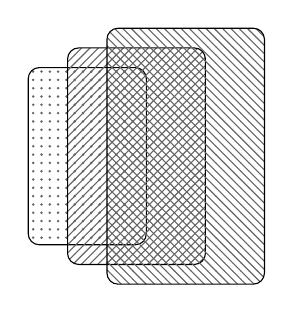
\begin{tikzpicture}
  \draw[pattern=dots, pattern color=black!60!white, rounded corners] (0,.5) rectangle (1.5,2.75);
  \draw[pattern=north east lines, pattern color=black!60!white, rounded corners] (.5,.25) rectangle (2.25,3);
  \draw[pattern=north west lines, pattern color=black!60!white, rounded corners] (1,0) rectangle (3,3.25);
\end{tikzpicture}

The third figure demonstrates the important of the agent's confidence in their ability.

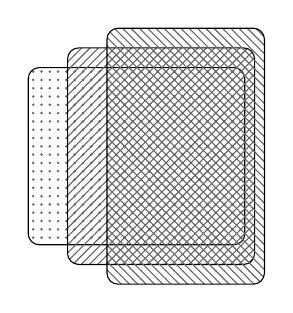
\begin{tikzpicture}
  \draw[pattern=dots, pattern color=black!60!white, rounded corners] (0,.5) rectangle (2.75,2.75);
  \draw[pattern=north east lines, pattern color=black!60!white, rounded corners] (.5,.25) rectangle (2.875,3);
  \draw[pattern=north west lines, pattern color=black!60!white, rounded corners] (1,0) rectangle (3,3.25);
\end{tikzpicture}

\newpage


Heck, this is almost \emph{exactly} what I want out of the student case.
I link together these, so the student gets confident in the basics, and then goes on to tackle.

The really devious case is where the second link breaks down with sufficient mastery of the basics.
Though this seems odd.

So, the goal is to establish ??? by outlining the construction of scenarios in which the informer \emph{only} communicates to the agent their ability to \(\phi\).
(In turn, scenarios in which \ref{i:claim:no-supp} would be a successful response to presumed support for \(\phi\) from the informer.)
Hence, the informer will not give enough information for the agent to have the option of obtaining support for the fact.

\citeauthor{Grice:1989uf}\footnote{
One of the Gricean Maxims of Quantity.
Do not make your contribution more informative than is required.

As the ability claim is something communicated, it may be the case that one do not have the option of communicating such restricted claim.

The other maxim of quantity.

Make your contribution as informative as is required.
}

Hence, the goal shift the burden, and show that the informer must be communicating more than they intend to if they are interpreted to have claimed the existence of a strategy.
Failed intentions happen all the time --- detective cases etc.
Still, possibility claim.
Push the restricted claim as strongly as possible through background considerations.

{
  \color{red}
  On the one hand, the informer may not have the option of sharing the support they have.
  Therefore, it seems the agent does not have the option of obtaining support if the agent were to seek some kind of transmission.
  And, one the other hand, the informer may not intend to provide the agent with support, and so avoids communicating any information that would provide support for the fact independently of what (necessarily) follows from making the ability claim.
}

\hozlinedash

\begin{note}[The things of interest]
  There are a few different propositions to distinguish between.
  \begin{itemize}
  \item That the fact is true.
  \item That the fact is true and the agent has the ability.
  \item That the agent has the ability \emph{given} the fact is true.
  \end{itemize}
  The thing to observe here is that the agent should be as confident that they have the ability \emph{given} the fact is true to the same degree that they are confident that the fact is true.
  If this is the case, then the agent is going to be slight more confident that the fact is true than they are confident that they have the ability and the fact is true.
  That is, unless they are certain that they have the ability.

  So, then, the dynamic is sort of unique in this sense.
  The point is that the agent may reflect on the basic nature of things and come to the conclusion that it's a little more likely that the fact is true than their ability to demonstrate given that the fact is true.
  So, that the agent is more confident that the fact is true is no argument \emph{against} the position that I am arguing for.

  Hence, one doesn't need independent support in order for the agent to lose confidence in truth `quicker' than ability in absolute terms.
  However, it doesn't follow that this works in relative terms.

  The key question is whether the ratio fails.
  Or, whether a loss of confidence in the conditional leads to loss of confidence in truth.

  Though, nothing is quite so straightforward.
  As there will be further considerations about how the ratio works.
  Hence, a strict equality is something of a simplification, the question is whether there is something of a function governing the ratio.

  Simple idea, really, is that drop in confidence leads to a drop in truth.
  And, one might think this is so.
  For, it doesn't seem as though there is sufficient information to separate.
  Very simple idea is that I can't, without something special happening, determine whether I'm showing that my ability is false, or whether the fact is false.

  The claim made by the informer doesn't seem to offer any sort of input here.

  The key objection is that \emph{somehow} the rolls point against both.
  So then, in a sense, the agent does have support for the fact.
  However,

  Hold up.
  There is an intuitive idea that the rolls point against the fact or the ability.
  Yet I have no idea how to make sense of this.
  For, from the agent's perspective this seems indeterminate.
  The agent needs some way of separating the two.
  This is exactly what happens in the homework cases --- the ability drops.

  You might think that, here, the same happens, but one gets to a stage where the failure to exercise the ability ends up dropping the confidence of truth.
  That's the real puzzle.
  If there is independent support, then it's hard to see why this should be the case.

  One possible explanation is that the agent gets into a position where the lose faith in the informer.
  So, the support for both claims ends up being hollowed out.

  \begin{itemize}
  \item In general, the inability to distinguish between two hypothesis given some evidence does not show that the two hypothesis share the same support.
    \begin{itemize}
    \item This is shown with a courtyard case, where to independent pieces of evidence, one with agent being in the courtyard, the other with bgent being in the courtyard.
      Information that only one person is in the courtyard.
      So, seems balanced between agent and bgent being in the courtyard.
      I can split the difference, but this doesn't show that I am unable to separate the two pieces of evidence.
    \end{itemize}
  \end{itemize}

  So, in the ability claim case, it could be that the agent has two independent pieces of support, and the failed rolls are inconclusive.
  Hence, until the agent doubts both, there's no reason not to grant the agent independent support for the fact.

  However, there still seems to be something of a dis-analogy.
  In the courtyard case, there's some confirmation.
  So, information is that one (or more) of the agents is lying.
  Then, no confirmation.
  Same upshot.

  Still, something seems different.
  For, there's some relation between the two propositions in the ability case.
  Know for sure that the ability claim is weaker.
  This demonstrated by the homework example.
  It's clear that in this case there is independent support, and therefore the agent only doubts their ability.

  And, the problem is that this does not seem to be the case when rolling the die.
  Here, it is possible that the agent is granted to sources of support.
  Yet, the agent, from their point of view, has no hope of distinguishing between the two.
  Which, should be enough, no?
  Yet the courtyard case is a puzzle, as it's clear the agent has independent sources of support without the option of leveraging.

  At the least, this is inconclusive.
  Both options work.

  Why not default to the weaker proposition, though?
  In part, because it's not clear that it \emph{is} a weaker proposition.
  The conditional may be just as a strong as the fact.

  Okay, main difference is that with the ability claim, in contrast to the courtyard case, I have a conditional.
  Here, I'm not sure whether this makes a significant difference, though.

  The contrast to the homework case is the most striking.

  The main contrast to the courtyard case is that there is a single source in the ability case.
  So I want to say something like, if a single source is providing two independent pieces of support, then the receiver should be able to distinguish between these.
  Otherwise, the source is providing (at best) interwoven support, and this fails to be independent in the appropriate sense.

  This is somewhat intuitive.
  Single source saying \(A \land B\) is different from independent source saying \(A\) and another \(B\).
  Single source may also mark \(A\) and \(B\) versus \(A \land B\).
  This is clear with doubt.
  But also with belief, as you can't infer whether \(A\) or \(B\) is significantly dragging down the conjunction.

  Hum, there's something interesting with the observation that the agent can be confident that the informer has made a correct ability claim, but doesn't come to view the fact as true.
  This, however, blocks the factive inference.

  Heck, this is a really important observation.
  It's clear that an ability claim \emph{in general} does not provide independent support.
  For, the agent can form a conditional and remain suspicious about whether they actually have the ability.
  Which is almost the exact position that I want.
  The puzzle really is in these cases, where the agent could be suspicious, but ends up endorsing the ability.
\end{note}


\hozlinedash


\begin{note}[Moving to the logic student]
  Here, slightly different.
  If able to \(\phi\) then able to \(\psi\).
  Mistake to infer \(\phi \rightarrow \psi\).
  I'm so confident that you lack the ability to show that \(\psi\), I've chosen an arbitrary \(\psi\) that is suitably out of reach.

  Conditional, but this doesn't really change anything in terms of the factive inference problem.
  Can reformulate the chess example in a similar way.
  If able to reason from chess then able to find strategy.
\end{note}

The particular support the informer has isn't support for the agent.
However, there is a clear route for the agent obtaining support.
So, here the agent it seems --- in contrast to pure reasoning cases --- does not have propositional support for the fact.

However, given the primary interest is with cases in which it seems plausible to think the agent does have propositional support, this point isn't so important.

Have a fairly clear way to interpret \ref{i:claim:no-supp}.
I did not pass on the background context.
As observers, we can see what the background context is.
However, the agent is in the dark.

This distinguishes the case from other potential failures of transmission, in which the relevant support is made available.
Either through the speaker providing the support --- though not necessarily endorsing it --- or from the context constraining.
Doctors and teachers are institutions positions.
There are some gaps here, but the differences are substantial.

There's no independent path, and no (explicit) statement of fact.

Ability to flip coins isn't quite right.
So there are two possible explanations for a distribution.
Either the coin is biased, and I flip like a normal person.
Or, the coin is fair and I flip in a strange way.
Deny the ability statement, so really I have no idea.
You're going to have to do some additional work in order to get me to hold an opinion about the bias of this coin.

{
  \color{red}
  This relates to the choice objection later.
  And, distinguishes the case from the pure reasoning cases.
  For, in the pure reasoning cases there is no real option if the agent has the ability.
}



Putting this together, form an argument for the restricted form of information.
As there is a difference, the informer \emph{only} claims the ability, and hence does not (in addition) provide support for the fact --- this is kept for the informer alone --- but this is permissible because the agent's ability ensures that it is possible for the agent to independently obtain support for the fact.

(If this works, the same can be said for the chess example, as I did not consider \emph{every} possible move for white, but you may feel the need to given your understanding of chess.
And, same for logic student, it's a different proof system, but the instructor has done soundness and completeness, so has support that the fact can be derived, and is confident that the student has a good grasp of the rules --- yes, some proofs turn out to be quite tricky, but requiring anything more than a high degree of confidence seems excessive.
Or, less charitably I jump and skip in ways that wouldn't work for the student.
I.e.\ back to `pure' reasoning.)

Before turning to whether this is possible, let us not that it is desirable.
Students in class, giving a hint.
I give the student some information, but refrain from providing any support.

\begin{note}[Student]
  The main problem with the no presupposition idea is that this does not seem to be the case in general.
  This is the case with the student.
  Here, I am doing my best to avoid providing the student with any justification \emph{other} than what they would obtain by witnessing some reasoning that they are able to perform.
  In doing so, I tie the agent's ability to perform the factive inference to their confidence that they have the ability.
  Hence, obtain the next statement emphasised as a description of these cases.
\end{note}

The goal of the interaction is clear.
I wish to provide the student with information that \(\phi\) follows from \(\Sigma\) without providing the agent with any independent support for this.

Intuitively, only the proof supports, but then someone like \citeauthor{Owens:2006tw} will suggest that I provide the students with access to my support, and the external pressures of not only believing but also providing a proof do the work.\nolinebreak
\footnote{
  And, if I were to give a conditional, then the factive inference is blocked.
}

So there are two parts here.
On the one hand, the informer does not have the option of sharing the support they have.
Therefore, it seems the agent does not have the option of obtaining support if the agent were to seek some kind of transmission.
And, one the other hand, the informer does not intend to provide the agent with support, and so avoids communicating any information that would provide support for the fact independently of what (necessarily) follows from making the ability claim.

There's is no knock down argument against expanding the basic position of \citeauthor{Owens:2006tw} here.\nolinebreak
\footnote{
But there's something of a problem.
The support I have for holding that this coin is `weakly' conflict with the support I have for my confidence that these other coins are fair/unfair.
However, this doesn't seem too compelling as it also seems to hold for memory, where the support drawn on for a memory may also weakly conflict with other propositions that the agent holds to be true.
}
The agent still `taps into' the support that the informer has, against the informer's intent.
However, in the logic case, for example, it's hard to draw a distinction between tapping into the support the instructor has, and tapping into the axiomatic system itself.

Distinction between propositional and doxastic justification, it's unclear.
It seems, at least, the given the ability claim the agent has something more than propositional justification, even if the agent simultaneously lacks full blown doxastic justification.\nolinebreak
\footnote{
  \textcite{Wright:2016wl} has a nice note about the usefulness of making the distinction between prop.\ and dox.\ just.\
  \begin{quote}
    The idea is that the speaker believing that \(\phi\) is a necessary condition of the speaker having a justified belief that \(\phi\), but it isn't a necessary condition of a speaker merely having justification for \(\phi\).
    And since justification transmission, \dots merely appeals to a speaker having justification for what she says, the speaker can have justification in the relevant sense by having a merely propositional justification for what she says.\nolinebreak
    \mbox{}\hfill\mbox{(\citeyear[10]{Wright:2016wl})}
  \end{quote}
}

Still, interested in ability due to agent's like us who do not have unbounded resources, etc.
So, let me tentatively push a stronger argument.

\begin{note}[Misleading]
  And what about `misleading' evidence with a third party?
  So, the informer gets some information from someone, the agent has misleading evidence that this person is no good.
  So, the agent would not endorse the support that the informer has, but what the informer states is true, the agent does have the ability.
  Therefore, the informer really does want to make the ability claim.

  This gets into a tangle.
  The factive inference looks risky.
  If I had information, then I may prefer to reject the ability claim.
  But the ability claim is true.
  And if the support is separate, then no particular problem.
  Hence, why the informer makes this particular claim --- as the informer is confident that the evidence you have against the third party is misleading.\nolinebreak
  \footnote{
    Maybe include a footnote here about wild beliefs, etc.
    Don't trust coin flips and do a physical measurement.
    Have some really strange chess beliefs that are so entangled that there is support is a sense, but it's really needs to be extracted.
    Hence, I really do think that the support you have is no good, but can be reformed to appropriately support the existence of a strategy.
  }
\end{note}

\begin{note}[Final intuition]
  The tracking example.
  Look, these are\dots but you have to take my word for it.
  Versus, these are\dots but you have to figure it out by yourself --- literary examples of this.
\end{note}


\begin{note}[Concluding note]
  Well, it seems to me that the extreme position here is that as the informer must believe that a strategy exists, etc.\ then this in itself is sufficient to taken as evidence that a strategy exists.
  \begin{itemize}
  \item If you have support, I have the same support.
  \end{itemize}
  So, the very claim itself is evidence that a strategy exists.
  But this is where the second objection comes in.
  For, if I can force this to come \emph{via} the ability claim, then there's still going to be sufficient circularity involved.
  In particular, with treating the ability claim as a form of evidence, etc.\
\end{note}

\begin{note}[Potential complication]
  \begin{enumerate*}[label=(\roman*)]
  \item The example may be made more complex.
    I claim that you have the ability to demonstrate that \(\phi\) follows from \(\Sigma\), and I have demonstrated that \(\psi\) follows from \(\phi\).
    I now claim that you are able to demonstrate that \(\psi\) follows from \(\Sigma\), as my reasoning was fairly simple, but I have not shown that \(\psi\) follows from \(\Sigma\), and therefore it would be a mistake to infer that I have stated that \(\psi\) follows from \(\Sigma\).
  \end{enumerate*}
\end{note}

\newpage

\subsubsection{The conditional is non-transmissive}
\label{sec:argum-non-transm}

\begin{note}[Overview]
  Have shown that the fact depends on the conditional.
  Now to argue in a little detail for the claim that the argument is non-transmissive.
\end{note}

The intuition is straightforward.
As the agent has not demonstrated the ability, they do not have support for the fact.

In endorsing the conditional, the agent presupposes that there is a strategy.

Sort of get the intuition a little cleaner in the twins case.
If it's Sam, then you'll be able to check.
Still bad.

Or,

If you have the general ability to distinguish between Leon and Noel, then you'll be able to decide who won the arm wrestle.

Fairly reasonable, but the issue is that you must be confident that you have a piece of information that you've overlooked.
If you don't assume this, then you have no reason to think the general ability extends to this case.

This is basically the same issue as noted in the original twin case, as expected.
{
  \color{red}
  Difference is that this hasn't been Incorporated yet.
  Confidence is high, but the agent isn't required to know.
}


\begin{quote}
  A body of evidence, e, is an information-dependent warrant for a particular proposition p if whether e is correctly regarded as warranting p depends on what one has by way of collateral information, I.

  Such a relationship is always liable to generate examples of transmission failure:
  it will do so just when the particular e, p, and I have the feature that needed elements of the relevant I are themselves entailed by p (together perhaps with other warranted premises.)
  In that case, any warrant supplied by e for p will not be transmissible to those elements of I.
  Warrant is transmissible in such a case only if a rational thinker could cite as her ground for accepting I the fact that she has warrant for p, supplied by e, together with the entailment.
  No rational thinker could do that if the warrant for p supplied by e originally depends on prior and independent warrant for I.
\end{quote}

Davies endorses:
\begin{quote}
  First Limitation Principle (revised version) Epistemic warrant cannot be transmitted from the premises of a valid argument to its conclusion if, for one of the premises, the warrant for that premise counts as a warrant only against the background of certain assumptions and acceptance of those assumptions cannot be rationally combined with doubt about the truth of the conclusion.
\end{quote}
Here, the background assumption is the existence of a strategy.
Doubt about this leads to doubt about ability, or whether to endorse the informer's claim.

In fact, ability claims \emph{never} transmit warrant.
This is because the agent lacks independent verification, and so presupposes the fact.
Or, the agent possesses independent verification, and the ability claim does nothing for the fact.


\begin{note}[Prop/Dox]
  Difficulty here is that it seems as though the agent must have the relevant propositional justification.
  However, these transmission principles are about the failure of propositional justification.
  This seems to block the straightforward application.

  So, in a sense, the reasoning would be a trivial failure, because the agent doesn't gain propositional support in virtue of their ability.

  It seems to me that the failure here is the \emph{in virtue of} requirement of doxastic justification.
  For, it seems that reasoning via ability doesn't establish the appropriate link between the propositional justification the agent has and the fact.

  Hold on, the thing is that there's a failure of transmission from abilities.
  This may be propositional.
  Oh, but the point is that this doesn't matter.
  For, the agent may still have propositional support.

  Still, in a sense this doesn't matter.
  Because, this shows that the agent doesn't get a reason.
  But tricky.
  It seems the goal was never to provide propositional support.
  This must be the answer? No?
  For, the goal could not have been to establish propositional support by this argument.
  Of course, this is hypothetical, but it would be a strangle goal.

  The agent was not attempting to establish that they were in a position to be confident that \(\psi\).

  So, it seems as though propositional support was not the goal.
  Question is whether the agent gains doxastic support?

  Intuitively, no.

  Failure of doxastic support because, as the ability has not been witnessed, there is the possibility of a mistake, and this, granting the conditional, undermines the initial premises, that the agent is able to reason well with the rules of chess.

  I'm somewhat confused about the Tucker paper.
  For, in these cases, it's not clear that there is a genuine transfer of warrant.
  Instead, it seems a repurposing of warrant.
  No, this doesn't make sense, as this is basically the idea of transmission.
  Or, maybe\dots
  For, think about shipping.
  Pack some stuff, and pass it over.
  This is my basic understanding of transmission.
  This is different from telling someone where to find something that has already been delivered to their dock.

  Doxastic justification muddies this, because it seems the agent did not believe.
  And, the distinguishing feature of doxastic justification is that it is involved with belief, rather than being in a position to believe.
  Hence, as the agent did not believe, the agent did not have doxastic support.
  And, as the agent's reasoning goes via the deduction, the support comes in virtue of the deduction.
  However, this assumes that doxastic justification is tied to a particular proposition, and I don't see a reason to think that this is true.
  This allows the doxastic support to be refurbished.

  Then, there's a problem with the ability being repurposed.

  And, we see that the support that the agent has for the general ability is not repurposed.
  In particular, because the new information revises the understanding of the general ability.

  See that the ball could not have been red without it being coloured, but it could have been the case that the agent had good support for general ability without having the specific ability.

  The support is separable, in the way that red and coloured are not.

  So, inclined towards the view endorsed by others about the relation, given the understanding of transmission involved.
\end{note}


\subsubsection{Path 2}
\label{sec:path-2}

\begin{note}[Logic example]
  The logic example would be nice here.
  For, it's clear that the instructor has some uncertainty about the student's grasp of the rules.
  And, neither wants to provide too much of a hint.
  So there's a back and forth about figuring out what the student is able to do.
  And the student may well reject the claim of the instructor --- \emph{for sure!}.
\end{note}

\begin{note}[\citeauthor{Emms:2000aa}'s problem]
  The same kind of thing works with \cite{Emms:2000aa}'s original problem, where it's really not clear that I have the ability.
  However, this is also going to be mentioned earlier in setting up the ability claim.
\end{note}

\begin{note}[Path 2 overview]
  General structure:
  \begin{enumerate}
  \item Informer is confident that agent has the ability.
  \item Some of the information is about what the agent is able to do.
  \item The informer's confidence is tied to the/contingent on information available to the informer.
  \item The informer does not, in general, have a superior position.
    \begin{itemize}
    \item If the agent were to signal otherwise, then barring confusions, the informer would revise their assessment.
    \item Chess is an example --- agent isn't aware that they know \emph{all} of the rules --- is there something similar to \emph{en passant} for knights?
    \end{itemize}
  \item It is therefore up to the agent to endorse the informant's position in some cases.
  \end{enumerate}
\end{note}

\begin{note}[Notes on path 2]
  This is a subjective evaluation.
  Given the information the informer has, the have this degree of confidence.

  So, as the agent and the informer may have difference information, the agent needs to also endorse.

  For example, you may know that you do not understand how knights move.
  The informer seems fine with the confidence that they have --- they've seen you work through a number of puzzles and the absence of any knight move was not particularly noticeable, but this has been weighing on your mind.

  Hence, something along these lines shows the need for additional endorsement on the part of the agent.

  However, with the requirement of some endorsement in hand, the agent can not support \(\phi\) being the case.
  This holds even for \emph{confidence} that \(\phi\) is the case, as the relation of support is constrained.

  So, this pushes for either licensing or no inference.
  An additional point to make here is that this is not the \emph{only} motivation for licensing.
  For, there is also the difference between preservation of a designated value and construction of a witness.
  So, this forms a pair of a necessary and a sufficient observation.

  So, either the agent does not have support, or the support is licensed.

  There's no straightforward argument that the agent has (licensed) support.
  Idealised agents aren't to useful here, as we may assume that the ability will be witnessed.
  For agents like us, however, it seems we can use ability in reasoning.
  Though it is risky.
\end{note}

\begin{note}[Does not hold for all cases of ability]
  This may not be true in all cases of ability.
  For example, coach telling an athlete that they are able to perform a particular routine.
  Here, the coach may be an authority.

  Same may be true in some cases of reasoning, though this is trickier, due to lack of certainty.
  Rule following, etc.
  But then it seems that perhaps both the agent and the informer would be unsure, and it would remain the case that the informer could still be in a position of authority.
  Hence, narrower claim.

  This is about comparative positions, then.
\end{note}

\newpage



\section{Licensing}
\label{sec:licensing}

\begin{note}[Guarantee]
  Note, this is compatible with the informer `being on the hook' for support.
I am inclined to think the agent is `on the hook', and so the agent may avoid endorsing the ability claim and request the informer provide support.
Maybe this would in turn provide the agent with support\nolinebreak
\footnote{
  Though not clear why this would be the case in general.

  May think that exercises without solutions are an example.
  Not quite.
  Details are in the following section.

  Perhaps the agent is piecing together different pieces of information.
  A has solved, B is at least as capable as A, hence B has ability, etc.
}
but even if this is granted, the agent may not wish to make the request of the informer.
The chess problem is simple, and on a good day there is some enjoyment to be had from this.

In turn, the informer may end up doing some work, if they aren't in a position to share the support they have.
Taking from the examples, the informer ends up flipping the coin with the agent, or working through the proof.
\end{note}

\begin{note}[Async]
  This is sort of the main idea here.
  The primary use is that there's the option for the agent to act on their confidence prior to witnessing the reasons.
  The agent then cites those reasons, but fills in the details at some later date.
\end{note}

\begin{note}[Required conditions]
  Need:
  \begin{enumerate}
  \item Information that some conclusion follows from some reasoning.
  \item Confidence that the agent is able to perform the reasoning.
  \end{enumerate}
  If both these conditions obtain, then the agent may be confident that they are able to generate an {\color{red} relevant kind of} explanation.
\end{note}

If you were to do the reasoning you are able to do, you would demonstrate a witnessing strategy for Black on the basis of the rules of chess and the game state.

\begin{itemize}
\item Note also that the ability claim would not be required here.
\item Here, witnessing what substantiates the ability claim.
\item So, would not have the problem noted above.
\end{itemize}

In this way, claim~\ref{chess:claim:1} may be understood as guaranteeing a relation between your ability to reason from the rules of chess and the game state to the demonstration of a strategy for Black.

\emph{License} to appeal to what ability would witness.
Factive inference is not supported by ability.
Instead, supported by the reasoning the agent is able to do.

Agent is in the dark about what this support is.

Need to be clear that the agent is not providing support for the conclusion.
This is where we obtain the denial of the main conditional.

As the agent does not claim to possess support for the conclusion, then the problem of circularity is avoided.
Yet, from this it does not follow that the agent does not claim the conclusion is supported.

Information about what the agent is able to do permits an agent to infer contingent on the agent witnessing the ability.

Put in terms of reasons.
The reasoning that the agent is able to do constitutes a reason for holding that a strategy for Black exists.
As the agent has not witnessed their ability.
Potential explanation.

One way to capture this is by rewriting.
For example:

\begin{enumerate}
\item\label{potential:claim} I am able to reason from the rules of chess and the game state to the proposition that White cannot prevent Black from occupying c4 on their second move.
\item\label{potential:necessity} The reasoning I am able to perform provides support for the proposition that White cannot prevent Black from occupying c4 on their second move.
\item\label{potential:focus} White cannot prevent Black from occupying c4 on their second move (is supported by reasoning I am able to perform).
\end{enumerate}

There's not really new information here.
The second step rewrites the first, and the conclusion rewrites the second step to focus on the relevant proposition.

If so, the factive inference is misleading.
Do not obtain the fact, but bring the fact into focus.

This is not completely satisfactory.

The interest of a factive inference is the possibility of independently reasoning with the fact.

Rearranging, or placing the agent's ability to establish the fact in parenthesis does not change the structure of the proposition.

Consider the following sketch:

\begin{enumerate}
\item Black's king is on c7.
\item Black cannot occupy c4 on their first move.
\item If White can place Black in check on their move, then Black would need to defend their king on their second move.
\item Moving a piece to c4 would not protect the king.
\item\label{sketch:MTCond} If White can place Black in check on their move, White can prevent Black from occupying c4 on their second move
\item\label{sketch:factive:premise} White cannot prevent Black from occupying c4 on their second move.
\item\label{sketch:conclusion} White cannot place Black in check on their move.
\end{enumerate}

It is not possible to replace step~\ref{sketch:factive:premise} with \ref{potential:focus} while maintaining valid reasoning.

For, the agent needs the fact that White cannot prevent Black from occupying c4 on their second move in order to perform \emph{modus tollens} on step~\ref{sketch:MTCond}.
That \emph{White cannot prevent Black from occupying c4 on their second move (is supported by reasoning I am able to perform)} only contradicts the consequent of step~\ref{sketch:MTCond} given the factive inference.



So, treat this as a propositional attitude on par with belief, desire, intention, etc.



The reasoning is then appropriate from the perspective of the agent.
From the perspective of us as theorists, we have a collection of propositions believed with a proposition licensed.


To say a little more here.
The ability statement is already a modal statement.
The distinctive claim is that this in some cases this takes the form of an attitude, and in turn the functional profile of the attitude determines how the proposition interacts with other propositions the agent has attitudes toward.


Agent holds the proposition true, but without claiming the possession of support for the relevant proposition.
It is bundled with a license.
This is the distinctive trait.

\begin{note}[License + Reasoning]
  Also note here about an indirectly licensed conclusion.
  However, part of the value here is that if the agent provides support for the licensed premise, then the agent obtains support for the indirectly licensed conclusion.

  This is a nice parallel to promises and futures.
\end{note}



\begin{note}[Prop/Dox]
  proposition.propositional/doxastic\nolinebreak
  \footnote{
    Frame this in terms of propositional and doxastic justification.
    Here, the agent has a guarantee that they have proposition justification, and that they can generate doxastic justification.
    However, the guarantee itself is not doxastic justification. }
\end{note}

\begin{figure}[h]
  \centering
  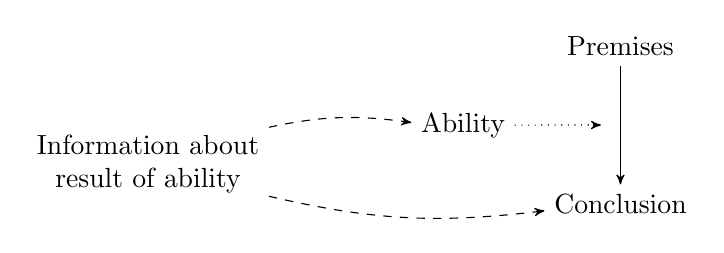
\begin{tikzpicture}[->,>=stealth',node distance=0cm, every text node part/.style={align=center}]

  \node (1) [] {Information about \\ result of ability};
  \node (2) [right of=1, xshift=4cm, yshift=.5cm] {Ability};
  \node (3) [above of=2, yshift=1cm, xshift=2cm] {Premises};
  \node (4) [below of=2, yshift=-1cm, xshift=2cm] {Conclusion};

  \draw [dashed, ->] (1) to [bend right=10] (4);
  \draw [dashed, ->] (1) to [bend left=10] (2);
  \draw [->] (3) to node[left] (mid) {} (4);
  \draw [dotted, ->] (2) to (mid);
\end{tikzpicture}
\caption{Sketch of support.
  Continuous arrow is direct.
  Dashed is indirect from information.
  Dotted is indirect from agent.}
\label{fig:dynamics}
\end{figure}


\begin{note}[Variation on a familiar problem]
  This is a twist on a familiar problem.
  Lots of ways to explain why an agent performed an action.
  Here, the agent is picking one of those ways.

  Problem is to identify the actual from the potential reasons.
  Here, our agent has a guarantee of potential reasons, and acts on the basis of those.
  If the agent could, then the agent is.

  With sufficient information about potential reasons, may an agent from appealing to those reasons when performing an action?

  justification footnote\nolinebreak
  \footnote{
    A different way to motivate the idea is through propositional and doxastic justification.
    As, the agent has a guarantee both that they are propositionally justified, and that they have the ability to be doxastically justified.
  }
\end{note}

Still, even though you would be able to demonstrate claim~\ref{chess:claim:2} without my testimony, my claim remains important in order for you to be confident that you have the ability --- even if you are confident that you understand the rules of chess and the game board, you would not be able to establish that White cannot prevent Black from occupying c4 on their second move without demonstrating a strategy for Black.
Claim~\ref{chess:claim:1} \emph{licenses} you to hold that claim~\ref{chess:claim:2} is true on grounds that are independent of my testimony.

Colloquially, you may cite the reasoning that you are able to do (or the strategy that would result from the reasoning) as support for holding that claim~\ref{chess:claim:2} is true.
And my testimony that claim~\ref{chess:claim:1} is true is then cited in support of your ability to do the reasoning.\nolinebreak
\footnote{
  Similar phenomena with `do you also hold \(\phi\) to be true?'
  Well, you hold \(\phi\) to be true, etc.
  So on the basis of you asking this, I may hold \(\phi\) to be true.

  Or, may reason to \(\phi\).
  So, alternative paths is not unique to ability attributions, though this differs in an important way, as you do not gain from this confidence that you can demonstrate that \(\phi\) is the case independently of the interaction.
}

{
  \color{red}
  facts we take into consideration in reasoning are reasons \\
  reasons as items in pieces of reasoning, where reasoning is thought (or possible thought) directed toward some conclusion (\citeyear[421]{Hieronymi:2011aa})
}
Reasons that reasoning took into account, then a distinction between the reasons which led to the conclusion and the reasons that the agent takes to support the conclusion.


Re-express the problem, the reasons why the agent holds that the Black has a strategy are those reasons that I (the agent) have the ability to reason with.

This cuts across both `normative' and `explanatory' uses of `reason'.
Why did the agent, in fact, act?
If the agent is appealing to those witnessing reasons, then they are part of the explanation.
If the agent is appealing to those witnessing reasons, then these affect whether the outcome was appropriate.

\hozlinedash



\section{Counterpart argument}
\label{sec:counterpart-argument}

The argument above is narrow.
Focused on the issue of whether or not the agent has support for a particular proposition.

Constrained so that the agent needed to endorse ability.
Hence could not obtain support.
These are the considerations I am inclined towards.
Support is important, but it does not necessarily need to be realised.

However, defensive.
May be that any realised support would do better.
The counterpart to the defensive argument is assuming that licensing is okay and suggesting when it may be preferred to realised support.

Scenarios, and then a big picture argument, where the big picture is different kinds of support.

\subsection{Failure Scenarios}
\label{sec:failure-scenarios}

\begin{note}[Failure scenario]
  Return to the logic classroom.

  \begin{itemize}
  \item If you are able to show \(\phi\), then by similar reasoning you are able to show \(\psi\).
  \item \(\phi \coloneq \exists x(Px \land Qx) \vdash \exists x(Px \lor Qx)\).
  \item \(\psi \coloneq \exists x (Px \land \exists x Qx) \vdash \exists x(Px \lor Qx)\).
  \item Student has some support for this --- whether the conditional holds isn't so important, so long as the agent is confident it does.
  \item The problem for the student is how the rules for instantiation work.
  \item Student isn't able to explain why the same instantiation on the two separate existential statements in \(\psi\) is bad.
  \item Tricky issue of whether the student really gets the antecedent of the conditional.
  \item Problem is that the result of luck doesn't seem to result in an ability.
  \item Still, sufficient grasp of working with single existential statements where no constants are involved.
  \item So I think it is fair to assume this --- if not, then things get difficult for most proofs --- not looking for mastery.
  \end{itemize}

  Student shows \(\phi\).
  Confident that the consequent holds.
  Hence, writes down \dots

  The student is correct, but the reasoning is not \emph{identical} --- different values for the distinct quantifiers.
  Instantiate, take the antecedent conjunction, and then introduce latter disjunct.
  Slight variation, and the student doesn't have the ability to show.

  This is suggested in a later proof, where the agent fails to appropriately use the rule.\nolinebreak
  \footnote{
    \begin{itemize}
    \item For example, \(Qa \rightarrow Ra, Pa, \exists x Qx, \forall x \lnot \exists y (x \ne y)\).
    \item Straight \(Qa\) for existential, with assumption of redundant premises.
    \end{itemize}
  }
  Let us stipulate that the student would obtain \(Pa \land \exists x Qa\).
  Rules governing quantifiers --- and quantifier scope --- are nuanced.

  Conditional doesn't hold because abilities are sufficiently distinct.
  Or, antecedent doesn't hold because success doesn't entail ability --- in contrast to exercising an ability, the student lucked the proof.

  Still, what the agent claimed is true, at least on a passable reading of `similar reasoning'.
  Instantiate the first existential, conjunction elimination, disjunction introduction, and existential generalisation.

  Student was unlucky, misled.
  Still, conditional/antecedent does not yield the conclusion without a factive inference from the agent's ability to show \(\psi\) by similar reasoning to the claim that \(\phi\) follows by similar reasoning.
  Misguiding confidence, but misguided confidence doesn't provide a complete picture.
  For example, thought it was going to be sunny today, but need to add that I left my umbrella behind to see how I was misguided.
  With the student, I claim, led the student to license reasons that they were not able to witness.\nolinebreak
  \footnote{
    May argue that the agent ought to have made the proof.
    Some fault for allowing student to make claims.
    Well, maybe.
    However, it seems as though ability statements can be used, and still have the problem of why the agent answered the problem in the way they did.
    And, agent was fine to be confident, hard to argue with this.
    If stakes are important, lower these as satisfactory.
    E.g.\ bonus problem, good grades, unneeded class, other things are more important, etc.
  }
  \hozlinedash

  The agent doesn't have the ability.
  The agent took the risk, and it didn't work out for them.
  The agent is not able to provide an explanation for the claim made.
\end{note}

\begin{note}[Factive reasons]
  This is somewhat similar to cases which suggest that reasons cannot be facts.
  Parallel in the sense that the agent needs to have the ability.
  Difference is the appearance/non-appearance of a reason.
  Similarity in the failure of an ability.
  However, if the similarity is pursued then difference is whether the agent possesses some input.
  Still, for now focusing on reasoning which involves explicit mention of ability.
\end{note}


\subsection{Three Positive Cases}
\label{sec:positive-cases}

\begin{note}[Cases]
  Here, deal with a number of cases.
  \begin{enumerate}
  \item Shopping \(\leadsto\) positing a simple relation between agents desire and action, tighten account of supporting reasoning.
  \item Detective \(\leadsto\) option of providing the support asynchronously.
  \item Temptation \(\leadsto\) agent's ranking of reasoning.
  \end{enumerate}
\end{note}


\subsubsection{Detective}
\label{sec:detective}

\begin{note}[Practical matters]
  I should include a note that the factive inference goes through, but it's up to the agent to figure out how to make use of this.
  Here, the potential may be insufficient.

  Similar, in some ways, to have evidence that would not be recognised by the court do to some administrative error (though this is not to say that not reasoning is the same as an administrative error).
\end{note}

\begin{note}[Async]
  Somewhere in here mention the idea of asynchronous reasoning.
  The reasoning doesn't (or reasons don't) necessarily stay potential.

  This ties to bounded agency, and part of the `why' question.
\end{note}

\begin{scenario}

  Case file contains evidence, but also notes made by Lewis.
  It is a mix, then, of the evidence that Lewis has gathered and inferences that Lewis has drawn.

  Morse looks through the case file.
  Does some reasoning.
  Makes use of the notes made by Lewis, so forms a conditional:

  \begin{itemize}
  \item If the case file is sound, then you are able to establish cause for bringing Woodthrope in for questioning.
  \end{itemize}

\end{scenario}

Morse provides information about an ability that Lewis has.


Note, this is not the same kind of conditional as in path 1.
For, the consequent of the conditional does not draw directly from an ability mentioned in the antecedent of the conditional.

Some remark on Lewis' ability is implicit, as notes are contained.
However, it does not follow that the reasoning demonstrated in these notes in the basis of Morse's claim.

The conditional could be false due to the ability claim.
The case file is sound, it does establish cause for bringing Woodthrope in for questioning, but Lewis does not have the ability to establish cause for bringing Woodthrope in for questioning.

Interest is in after the consequent is detached.
Lewis is confident that the are able to establish cause for bringing Woodthrope in for questioning.
Path 2, but the scope is a little different.
The reasoning made by Lewis is analogous.

The structure of the conditional is difficult for the two alternatives.
Morse has the ability, but Morse has not reasoned to the fact.
Similar considerations suggest that transforming Morse's claim into an assertion

Lewis endorses Morse's evaluation of Lewis' ability.
Additional practical consideration --- Lewis needs to be confident that they are able to establish cause.



Reasoning is a little more complex.
Morse has provided a conditional --- Morse has not checked the inferences made by Lewis.
Lewis is in a position to endorse the case file --- evidence and inference alike, and then perform the factive inference.


Morse has done more reasoning, Lewis has done less.
More could be more helpful, and Lewis could be less reliant.



\subsubsection{Shopping}
\label{sec:shopping}

\begin{note}[Also include\dots]
  A note on having a stack of papers that one starts reading through.
\end{note}

\begin{note}[Difference between chess and shopping]
   The issue is that the agent hasn't worked through the reasoning --- \emph{not} that the agent is unaware of the reasoning required.
  This is an important distinction between the chess scenario and the shopping scenario.
\end{note}

\begin{note}[Main point]
  The key with this scenario is the simplicity of the explanation.
  If agent is in the clear, then this is because they have the supporting desire.
  If the agent is in a bind, then this is because they do not have the supporting desire.
  So, we don't need to fluctuate desires.

  Also something to the idea of an explanation.
\end{note}

The existence of chess strategies is, at least for most, uncommon and with little practical consequence.
Confidence of the ability, so can go to sleep, or as a way to provide assistance without providing novel information.
Also, two agents involved.

First scenario is common, practical consequence, and single agent.


\begin{scenario}[Shopping]

  Background:

  Friend recommends trying carambola.
  Agent forms a desire.
  Does some research.
  Carambola and star fruit are the same thing.
  Hence, desire for star fruit.
  Purchasing as a means to this end.
  Writes a note on the shopping list.

  Out shopping.
  Sees star fruit.
  Does recall carambola.
  Does not recall that carambola and star fruit are the same thing.
  Confident that they are able to reason from a desire that they have to purchasing star fruit.
\end{scenario}

\begin{note}[Required conditions]
  Here, the shopping list provides the first required condition, and some nebulous considerations support confidence that the agent has the ability to do the reasoning again.
\end{note}


\subsubsection{Weakness of will}
\label{sec:weakness-will}

\begin{note}[Idea]
  This combines idea from the previous two.
  From shopping, the idea of preferable explanations, but now from the viewpoint of the agent.
  From detective, the idea of providing the appropriate reasoning at an other point of time, here from the past --- or potentially the future/counterfactual perhaps.
\end{note}

\begin{note}[Counterfactual]
Also could be framed as counterfactual ability.
Cases of rational impairment and so on.

In a sense, the issue here is the strength of the conclusion.
It seems the conclusions obtained while sober often extend and hold when intoxicated.

However, by contrast, conclusions obtained with full information may not.
E.g.\ \cite{Smith:2004aa} or the miners paradox.
\end{note}


\begin{note}[Different types of reasoning]

  The reasoning performed by the agent may be characterised as the \emph{preservation of a designated value}, where the designated value is \emph{truth}.
  For, if certain premises are true, then the conclusion is also true.

  This is distinct from the reasoning that the agent is able to perform, which may be characterised as the \emph{construction of a witness}.\nolinebreak
  \footnote{
    The relation here is similar to a position advocated by \citeauthor{Prawitz:2005aa}:
    \begin{quote}
      In the same vein, the assertion of a sentence is understood constructively as the claim that there is direct evidence for it, and is to be taken as true if such evidence exists.
      In mathematics the truth of a sentence thus becomes equated with the existence of a canonical proof or argument for it.\nolinebreak
      \mbox{}\hfill\mbox{(\citeauthor[692]{Prawitz:2005aa})}
    \end{quote}

    A nice quote from \textcite{Broome:2013aa}:
    \begin{quote}
      Facts that merely entail that an agent ought to perform the action are not necessarily reasons for her to perform it; to be reasons they must explain why she ought to perform it.\nolinebreak
      \mbox{}\hfill\mbox{(\citeyear[51]{Broome:2013aa})}
    \end{quote}
  }\(^{,}\)
  \footnote{
  To help illustrate the difference between the preservation of a designated value and the construction of witnessing reasoning, consider what Achilles said to the Tortoise:
  \begin{enumerate}[label=(\emph{\Alph*}), ref=\emph{\Alph*}]
     \setcounter{enumi}{2}
    \item\label{achilles:C} If~\ref{achilles:A} and~\ref{achilles:B} and true,~\ref{achilles:C} \emph{must} be true.
  \end{enumerate}
  Where A, B, and Z are:
  \begin{enumerate}[label=(\emph{\Alph*}), ref=\emph{\Alph*}]
  \item\label{achilles:A} Things that are equal to the same are equal to each other.
  \item\label{achilles:B} The two sides of this Triangle are things that are equal to the same.
    \setcounter{enumi}{25}
  \item\label{achilles:Z} The two sides of this Triangle are equal to each other.
  \end{enumerate}
  The Tortoise does not accept~\ref{achilles:C}, though the Tortoise does accept that~\ref{achilles:A} and~\ref{achilles:B} are true.
  The response of Achilles, \ref{achilles:C}, asserts that truth is preserved when moving from~\ref{achilles:A} and~\ref{achilles:B} to~\ref{achilles:Z}.
  Still, even if truth is preserved from~\ref{achilles:A} and~\ref{achilles:B} to~\ref{achilles:Z}, the Tortoise has a point --- preservation of truth is only useful is there is a guarantee that truth is in fact being preserved, and \emph{If you accept~\ref{achilles:A} and~\ref{achilles:B} and~\ref{achilles:C}, you must accept~\ref{achilles:Z}} is no more of a guarantee that~\ref{achilles:Z}.
  Carrol doesn't say --- or Achilles does not attempt to see -- what the Tortoise would have made of the following (sketched) reasoning.
  \begin{itemize}
  \item Let two sides of this triangle be labelled \(s_{1}\) and \(s_{2}\).
  \item As~\ref{achilles:B} is true, we know that there is some thing, say \(s_{e}\) equal to both \(s_{1}\) and \(s_{2}\).
  \item As both \(s_{1}\) and \(s_{2}\) are equal to \(s_{3}\), we see by~\ref{achilles:A} that \(s_{1}\) and \(s_{2}\) must be equal to each other.
  \item Therefore~\ref{achilles:Z} is the case.
  \end{itemize}
  The Tortoise may object to a step in this reasoning, though it is unclear whether they would as Achilles insists on convincing the Tortoise that~\ref{achilles:Z} must be true when~\ref{achilles:A} and~\ref{achilles:B} are true without working through the relation between the contents of~\ref{achilles:A} and~\ref{achilles:B} and the contents of~\ref{achilles:Z}.
  Perhaps the Tortoise does not accept that the two sides of the Triangle are equal to each other, or perhaps the Tortoise is seeking a demonstration of why the two sides of the Triangle are equal to each other that follows from the contents of~\ref{achilles:A} and~\ref{achilles:B}.

  So, one may hold that~\ref{achilles:C} is of interest only to the extent that certain things about equality and this Triangle conspire to make it so that the two sides of this Triangle are equal to each other.
  These things can be ignored if one grants that there is preservation of truth from~\ref{achilles:A} and~\ref{achilles:B} to~\ref{achilles:Z}, but the preservation of truth follows from those things, and can not be substituted for them.

  Hence, the Tortoise may refuse to accept~\ref{achilles:C} so long as the Tortoise is unclear on how equality and this Triangle are related, as the preservation of truth is merely a byproduct of whatever that relation is.
  The (sketched) reasoning, in turn, provides the Tortoise with an account of what truth is, at least with respect to these premises

  (Note that this is analogous to the rules of chess, game state, and possibility in the opening scenario.)
    {
    \color{red}
    \begin{enumerate}[label=(\emph{\Alph*\('\)}), ref=\emph{\Alph*\('\)}]
    \item\label{Achilles:Chess:A} Starting with game state and following the rules of chess.
    \item\label{Achilles:Chess:B} Black moves from d7 to e5 and then from d7 to c4.
      \setcounter{enumi}{25}
    \item\label{Achilles:Chess:Z} Black has occupied c4 without an opportunity for White to prevent Black from occupying c4.
    \end{enumerate}
    Hence:
    \begin{enumerate}[label=(\emph{\Alph*\('\)}), ref=\emph{\Alph*\('\)}]
      \setcounter{enumi}{2}
      \item\label{Achilles:Chess:C} If~\ref{Achilles:Chess:A} and~\ref{Achilles:Chess:B} are true, then~\ref{Achilles:Chess:Z} must be true.
    \end{enumerate}
    And so on\dots
  }
}

  Simply put, the reasoning that the agent performed guarantees that a strategy for Black exists as it must be true that a strategy for Black exists (if certain premises are true).
  The reasoning that the agent is able to perform, by contrast, would provide a particular strategy for Black, a witness for the existential statement that a strategy for Black exists.

  So, if the agent holds their ability as support, then this is a different kind of reasoning from the reasoning they performed.

  I am inclined to treat the construction of a witness as something more important, but for present purposes it is a contingent feature made to illustrate.
  Here, simple observation that the support is different.
  If the agent appeals to the reasoning that they are able to do in support, then the agent is appealing to support that differs from the reasoning they have performed.

  If so, then from the agent's point of view there is a divergence between the reasoning that led to the conclusion and the reasoning which supports the conclusion.

  {
    \color{red}
    It is important that these types of reasoning differ.
    However, it is only important in so far as the provides a way to distinguish and motivate interest in the reasoning that the agent is able to do.
    Motivate as intuitively there is something else, and distinguish as a clean line helps (in what way?)
    There may be cases in which the agent's ability to preserve a designated value is of interest.
  }
\end{note}

\section{Resistance}
\label{sec:resistance}


\subsection{Voluntarism and Hobson's Choice}
\label{sec:non-voluntarism}

\begin{note}[Grr]
  I think this belongs in the objection section, which might also help with structure.
  For, the worry here is that licensing reasoning is a form of voluntarism.
  One the one hand, I do not claim that the result of licensing is belief.
  Still, it seems to me this is relatively open --- functionally similar.

  Idea would be that reconstruct \citeauthor{Weatherson:2008uq}, hence obtain that licensing is voluntary, and therefore there is a problem with applying the factive inference?
  For, this involves a choice made by the agent, and that goes on to block any factive inference where the proposition is suitably independent.

  This is also somewhat suggested by the \citeauthor{Davidson:2001aa} motivation, where in a way there's a suggestion of the agent picking the reasons to believe something ---- however this in part focuses on the why and not the which.

  This is not to say that it is not possible for the agent to make the factive inference, but that it is not sound to do so.
  Right, kind of get the intuition that the agent would withdraw the factive inference if they were to reconsider the possibility that the carton in the fridge is empty.

  Then, the response is that it is a mistake to think that exercising the capacity is important in these cases.
  For, to the agent there is no issue of self control.
  For, in these cases the agent is confident that things would not go otherwise.
\end{note}

\begin{note}[Broad outline]
  The debate around voluntarism is difficult.
  What belief is, what voluntarism requires, whether cases can be excluded, etc.\
  Hence, unclear on what one obtains by voluntarism.
  Whether one has control over doxastic states.
  Whether there are deontic parallels between beliefs and actions.
  Understanding of justification.

  I am not inclined to take an absolute position, but I think that ability limits any voluntarist position in which failure to exercise a capacity to reason amounts to a voluntary act.

  Here, \citeauthor{Weatherson:2008uq}.

  \begin{quote}
    These conclusions that we leap to are voluntary beliefs; we could have avoided forming them.
    And not only could we have avoided these formations, but we would have if we had followed the methods for belief formation that we approve of.
    That seems enough, to me, to say the formation is voluntary.\nolinebreak
    \mbox{}\hfill\mbox{(\citeyear[10]{Weatherson:2008uq})}
  \end{quote}

  Checking the fridge, keeping counterexamples in mind, and so on.
  \citeauthor{Weatherson:2008uq}'s argument, roughly, is that these cases involve failure to exercise a capacity, and whether to exercise the capacity to reason is up to us.

  Argument, roughly, is that if an agent is confident in their ability to reason, then the agent is confident that they could not have avoided forming them.

  Obtaining a conclusion by licensing reasoning is not the same as failure of self-control.


  Extreme cases, like \citeauthor{Ginet:2001aa} I have nothing to say about.
  However, cases such as those suggested by \citeauthor{Weatherson:2008uq}.
  Here, following approved methods is not so clear.
\end{note}

\begin{note}[The factive inference]
  I do not assume that the factive inference results in belief.
  \url{https://iep.utm.edu/doxa-vol/} has relies on Ginet, where acceptance or acting as if true seems appropriate.
  And, I think so parallels could be drawn between my cases and those Ginet discusses.

  So, this provides a kind of voluntarism, but suggests a finer issue than Ginet notes.
\end{note}

Interested in inferential \(\phi\) for which the factive inference can be made.

Plausible link:
\begin{enumerate}
\item Agent may believe \(\phi\) only if agent is able to reason to \(\phi\).
\end{enumerate}

Stronger:
\begin{enumerate}
\item Agent may believe \(\phi\) only if agent is confident that they are able to reason to \(\phi\).
\end{enumerate}

The `may' of the antecedent can be read as rational permissibility, etc.

Indirect argument is that an agent is able to believe \(\phi\) only if the agent has reasoned to \(\phi\).
Therefore, it seems the agent must be confident that they are able to reason to \(\phi\), as if the agent is not confident that they have witnessed their ability, then the agent would doubt that \(\phi\) is the case.
So, this isn't interesting if an agent believes that \(\phi\).

However, this won't do for investigating voluntarism.
First issue is that choice may be part of the reasoning the agent is confident that they are able to do.

So, the appropriate reading of reasoning here needs to exclude choice.
Yet, in doing so this assumes that voluntarism is false.


\begin{enumerate}
\item If it is not the case that an agent is confident that they are able to reason to \(\phi\), then it is not the case that the agent may believe \(\phi\).
\end{enumerate}

\begin{note}[Justification]
  The key idea with \citeauthor{Ginet:2001aa} is that sometimes a person was not justified in holding a belief.
  And, this seems to entail that the person had the choice to make the belief.

  This, then, is similar with \citeauthor{Weatherson:2008uq}, where justification is optional.

  So, justification, therefore voluntarism.

  Quick argument is:

  \begin{enumerate}
  \item (Agent was not justified.)
  \item Agent ought not have.
  \item Agent could not have.
  \item Agent had a choice.
  \end{enumerate}
  Therefore, voluntarism, at least in some cases.
  \citeauthor{Ginet:2001aa} is somewhat explicit about this.
  \citeauthor{Weatherson:2008uq} is similar, something the agent ought to have done, and therefore the agent had a choice.

  With \citeauthor{Ginet:2001aa} we have lack of justification.
  So, if a requirement of justification is placed for rational belief, then these cases are going to fail.
  With \citeauthor{Weatherson:2008uq} we have partial justification.
  And, as this is non-monotonic, same idea.

  Inclined to agree that the agent had a choice.
  However, it does not follow from this that it appeared to the agent that they had a choice.
\end{note}

\begin{note}[Weatherson]
  It seems that \textcite[10]{Weatherson:2008uq} suggests that we leap to these conclusions, and that if we follow reasoning patterns that we approve of, then we would not perform these leaps.
  Hence, a key part of the argument for these being voluntary (though not volitional) is that these inferences are akin to losing one's temper.

  However, if ability is added, then these are not cases similar to losing temper.
  For, one is not failing to perform some reasoning that would otherwise be done, but taking a license for the reasoning.
  The agent makes a mistake in licensing these reasons, but this, I think, blocks some of the appeal of the argument.
\end{note}

\begin{note}[Link to belief]
  Hence, \citeauthor{Ginet:2001aa} isn't quite correct.
  The agent is able to reason to at most one, and it is a mistake to think otherwise.
  Still, \citeauthor{Ginet:2001aa}'s diagnosis is on point --- the agent does \emph{stake} something.

  \begin{quote}
    There are all sorts of beliefs that we form in haste, where we could have stopped to consider the various realistic hypotheses consistent with the evidence, and doing so would have stopped us forming the belief.\nolinebreak
    \mbox{}\hfill\mbox{(\citeyear[10]{Weatherson:2008uq})}
  \end{quote}
  Here, and in the following, \citeauthor{Weatherson:2008uq} focuses on exercising a capacity.

  However, there is a contrast with \citeauthor{Weatherson:2008uq}, who assumes, it seems, that the agent has performed sufficient reasoning, and questions whether the agent `should have' performed more reasoning.
  This then really does seem to be a case of voluntarism, as the agent decides where to stop, but going further may reverse the evidence --- but then unclear why this doesn't also apply to perceptual experience, as this may also be cut short.

  Also issue of how things appear to the agent.
  Noting that things could have gone otherwise doesn't seem compelling.
  Argue that here the agent was either irrational or did not observe a choice.
  So, \citeauthor{Weatherson:2008uq} may be right, in that things could have gone otherwise, but it's hard to square this with \emph{choice}.
  In a sense, the agent made a choice, but it seems something of a Hobson's choice.

  The point about perceptual beliefs is somewhat interesting.
  Need a case in which one could have avoided seeing something.
  So, think of an optical illusion, two lines appear to be the same length.
  Option of not seeing this.
  It is not clear to me where the difference is.

  However, this is achieved is by way of uniqueness.
  When there are multiple options, the same principle applies, but without much consequence.
  E.g.\ choosing cereal.
\end{note}

\begin{note}[Main idea]
  The point about non-voluntarism can be held independently from the broader point that I want to make.
  For, this is about restricting the choices of an agent, rather than providing the agent with choices, roughly stated.
  Hence, lack of ability make block, but it does not follow from this that instance of abilities opens.

  \begin{itemize}
  \item \emph{Therefore} I don't have anything robust to say about \emph{doxastic} voluntarism.
  \item Still, in these cases it's not clear that there is really voluntarism.
  \end{itemize}

  However, similarity in the sense of potential reasoning.
\end{note}

\begin{note}[What voluntarism is]
  The basic idea with non-voluntarism is that the agent does not have the option to form certain propositional attitudes.
  Primary case is belief --- \emph{doxastic} voluntarism (though the general idea extends to any attitude which may be the conclusion of reasoning).
  Motivating example: ???
\end{note}

\begin{note}[Something odd]
  Here, there's some odd.
  For, if focus is on cases where the agent does not have the ability, then this doesn't provide support for holding the opposing attitude.
  Unless, one has an exclusive disjunction.

  So the core idea here is that because the agent doesn't have the ability for, say, the negation, the agent does not obtain the particular attitude by volition.
  So, the key here is thinking in terms of conclusions of reasoning.
  Non-voluntary because exclusive conclusion, and the agent does not have the ability to reason to one of these.
  Doxastic stuff is interesting then, because it seems there is a unique attitude determined by the agent's evidence, whether belief, suspension, or disbelief.
\end{note}

\begin{note}[Hum]
  So the idea behind this kind of non-voluntarism is that the agent doesn't have the ability to reason to a particular conclusion.
  However, this isn't a good account of non-voluntarism and it doesn't say anything about what the agent does reason to.
  So, choosing breakfast cereals at the supermarket.
  Don't have the ability to reason to the conclusion that some particular cereal is any good.
  However, whatever cereal I do choose, it seems I do so voluntarily.
\end{note}

The main focus of the paper has been indirect access to reasons.

With non-voluntarism, the same ideas apply, but rule out certain conclusions.

It's the denial of an existential.

If the existential provides access and allows a conclusion to be adopted, and this holds in converse, then we've got a clear account of when an agent does not have the option of adopting a conclusion.

Hmm, there are two instances of this claim:
\begin{enumerate}
\item Adoption requires ability, hence if no ability then no option to adopt.
\item Ability along with exclusivity rules out certain options.
\end{enumerate}



\newpage

\printbibliography


\newpage

\section{Old notes}
\label{sec:old-notes}

The main motivation here is the common use of the idea of responding to reasons.
In particular, there's \citeauthor{Lord:2018aa} and others who hold the identity these, or \citeauthor{Broome:2013aa} with enkrasia, \citeauthor{Hieronymi:2018aa} with considerations, and others.
Representationalism and dispositionalismn, roughly.
If the proposition is true, then there's pressure.

\begin{note}[Functional role/function]
  The function of the attitude is (in part) determined by the reasons for which it is held.
  Individuate attitudes by their functional role, but an attitudes functional role does not (completely) determine its function.
\end{note}

\begin{note}[Quick argument]
  Quick argument is that reasons require direct response of a kind.
  Though I think I need to say more about direct response for this to be of interest.

  The basic idea is that without direct response there's no difference between the reason obtaining and the reason not obtaining, from the agent's point of view.
  In this sense, the argument is similar to those that could be made against certain forms of responding directly to reasons, etc.

  The response to this is that the second premise is false.
  But if this is the case then superveniece is false.
  So, I should use superveniece in the argument!

  And, the `insight' is that this is replaced by supervenience on mind + ability, roughly stated.
  The difficulty with ability is that this is not something that depends on the agent's mind, so to speak, because whether the agent is able to do something depends on how the world develops.

  Right, although the argument here is similar to the one used against Lord and co.\ it is not clear that it generalises.
  This is because I depend on the role of ability, and without this there is no argument.

  The argument against this, the one that suggests this is a framework issue, is that one may consider an agent's perception of their abilities to be sufficient.
\end{note}

\begin{note}[Schroeder]
  \textcite{Schroeder:2011aa} seems to argue for something similar.
  Roughly, don't need justification, just need guarantee that there are no defeaters.
  So, whether or not a belief is rational to have is down to whether or not there are defeaters.
  Hence, when we look at reasons, we end up looking at whether or there is defeat available.
  And so one `has' evidence in the sense that one lacks defeaters.

  So, quick summary is that:
  \begin{itemize}
  \item Justification entails defeats.
  \item Defeat is other reasons.
  \item Satisfy no defeat condition in other ways.
  \item In particular, by grating that other things can provide reasons.
  \end{itemize}

  This is quite similar to \citeauthor{Lord:2018aa}'s idea about comparative rationality.

  The trouble is that this allows an agent to go undefeated in what appear to be problematic ways.
  \textcite{Schmidt:2019aa} has an illustration with implicit biases.
  Here, as the agent fails to recognise some things as reasons, as problematic attitude is justified through lack of defeat in a way that it would not be if there were stronger requirements on justification.

  Here, I'd render the implicit bias as a search for ``talent''.

  As I don't say what it is for something to be a reason, I don't need to adopt \citeauthor{Schroeder:2011aa}'s position.
  I am only arguing for the claim that the agent obtains the result through a license.

  I may appeal to a similar idea --- in that an agent has a way to avoid defeat --- but I may differ in how this is established.
\end{note}

\section{Motivating quotes}
\label{sec:motivating-quotes}

Reasoning may not be necessary to respond to reasons, depending on how reasons are understood.
For example, the thin paper of a freshly printed book may be reason to perform a frictive raise of a page by thumb and finger in place of exposing the edge to one's fingertip.
Paper cuts hurt.
Still, I may do so as an instinctive response to the texture of the paper --- without reasoning.


for reacting for a sufficient normative reason
\begin{quote}
  A \(\phi\)s for a sufficient normative reason r just in case A’s \(\phi\)-ing is sustained or produced by the fact that r is a sufficient normative reason to \(\phi\).\nolinebreak
  \mbox{}\hfill\mbox{(\citeyear[142]{Lord:2018aa})}
\end{quote}

\begin{quote}
  Manifest Sufficient: What it is for A to \(\phi\) for a sufficient normative reason to \(\phi\) is for A to manifest knowledge about how to use r as the sufficient reason it is to \(\phi\).\nolinebreak
  \mbox{}\hfill\mbox{(\citeyear[143]{Lord:2018aa})}
\end{quote}

It seems that if the agent does not reason, then they do not react.

Follow up claim is that an agent is rational only if they \(\phi\) for a sufficient normative reason.
Rationality will be set aside, or at least put out of focus.
Interested in how an agent may be rational, arational, or irrational.

Similar claims:

\begin{quote}
  (R1\('\)) for an agent to C based on reason R involves not merely the agent’s representing R as justifying C---it also involves \emph{this latter representation (or its content) being part of the reason why the agent C's}.\nolinebreak
  \mbox{}\hfill\mbox{(\citeyear[197]{Neta:2019aa})}
\end{quote}

\begin{quote}
  (D1\('\)) \emph{basing} C on R involves the agent's exercising a disposition to C when both of the following conditions obtain: R, and the rest of the agent’s beliefs cohere with the proposition that R justifies C'ing.\nolinebreak
  \mbox{}\hfill\mbox{(\citeyear[194]{Neta:2019aa})}
\end{quote}

In order for the agent to exercise their disposition, there must be some contact between the agent and the reasons.

(Might be able to fit externalism in here.)

\begin{quote}
  (Possessed Reasons) S possesses an epistemic reason that p to believe that q if and only if (1) that p is an epistemic reason to believe that q, and (2) S justifiably believes that p or S has a basic presentational attitude that is not in need of justification with the content that p.\nolinebreak
  \mbox{}\hfill\mbox{(\citeyear[5]{Schmidt:2019aa})}
\end{quote}

\section{Somewhere notes}
\label{sec:somewhere-notes}

\begin{note}[The Secret Garden]
  \citeauthor{Lackey:2008aa} quotes \emph{The Secret Garden} "You can do it!" (\citeyear[22]{Lackey:2008aa}) and doesn't do much with this.

  \citeauthor{Lackey:2008aa} suggests that no information is passed.
  \url{https://ndpr.nd.edu/reviews/learning-from-words-testimony-as-a-source-of-knowledge/} suggests this is unattractive.
  I'm inclined to think we often say unattractive things.

  Even put attractively, this likely is not an instance.
  Colin would seem to have some independent support.
\end{note}

\begin{note}[Dox and Prop]
\begin{quote}
  Propositional Justification (PJ): S has propositional justification to believe that p iff S has sufficient epistemic reasons to believe that p.

Doxastic Justification (DJ): S has a doxastically justified belief in p iff (i) S has propositional justification to believe that p, (ii) S believes that p, and (iii) S’s belief in p is appropriately connected to S’s sufficient epistemic reasons to believe it.
\end{quote}
No doubt that the agent has propositional justification in the pure reasoning cases.

{
  \color{red}
  This is nice, but switch to support in order to avoid stepping on toes.
}

{
  \color{green}
  This is actually really important.
  For, I can't simply talk about support, as with the pure reasoning cases, it seems as though the agent does have the relevant propositional support.
  The point is that this will hook up only by reasoning.
  Therefore, one the one hand marking this distinction helps identify where (part of) the puzzle is.
  And, on the other, I can avoid worries about whether or not the agent `has' evidence, as this may be granted so long as the evidence is `only' propositional.

  The way this helps, however, is somewhat subtle.
  It means, in the first part of the argument, I don't need to rule out any transfer of justification.
  I only need to rule out transfer sufficient for doxastic justification.
}

\begin{enumerate}
\item Dox(Able(P))
\item Dox(P \(\rightarrow\) Q) \(\rightarrow\) (Dox(P) \(\rightarrow\) Dox(Q))
\item Dox(Prop(P)) \(\rightarrow\) Dox(P)
\item Able(P) \(\rightarrow\) Prop(P)
\item Dox(Able(P) \(\rightarrow \) Prop(P))
\item Dox(Able(P)) \(\rightarrow\) Dox(Prop(P))
\item Dox(Able(P)) \(\rightarrow\) Dox(P) [second, with previous]
\item Dox(P)
\end{enumerate}

The problem comes with different basis for doxastic justification.
Hm, this is difficult.

Here, one looks at the evidence, and sees the implication.
However, one doesn't yet have doxastic justification for each of the premises.
Hence, doxastic justification in the conditional.

One then goes and establishes the premises on a different day.
So, doxastic justification for implication and doxastic justification for premises.
But these are disconnected.

The same problem with ability.
Doxastic justification, even from a doxastically justified entailment isn't automatic.

So, this is a problem with the first premise read as P being sufficient to obtain Q.

However, when read as Q being necessary for P, then the first premise seems okay.
If you see that P requires Q, then it must be the case that you have doxastic justification for Q prior to doxastic justification for P.

When read as necessary conditions, then the problem arises.
The agent already needs to have doxastic justification for the fact.
However, denying the second premise is an option.
Then the penultimate step is trivial, no information is acquired.
Partial analysis of ability.

So, what I end up providing is a two part argument against the second step.
It's possible for the agent to be aware of having propositional justification, without also having doxastic justification.
However, as suggested, there doesn't seem to be ground for preventing the agent from appealing to that propositional justification.
\end{note}


\begin{note}[The informer's belief]
  This is something I have overlooked.
  For, I need to grant that the informer has the belief.
  And, then the informer has in a some better position.
  So, this is perhaps sufficient for evidence that the proposition is a fact.

  Denying this seems fairly implausible.

  If so, then denying support fails.
  For, the informer ends up providing support by virtue of making the ability claim.
  It doesn't matter whether the support that the informer has is support that would work for the agent.
  It remains that the informer's confidence of the fact must be at least the confidence that the agent has the ability.

  This is then quite elegant.
  If it is okay for the agent to be confident that the have the ability, then as the informer must also believe to sincerely make the ability claim, the informer's epistemic position then serves as evidence for the fact.

  Hence, the factive inference is avoided.

  Okay, this is an interesting problem.
  Where does it fit?

  Here, it seems as though the information is now coming solely from the ability claim.
  So, we are supposing that the ability claim is appropriate, and then inferring that the agent then provides support.

  Hence, it seems as though this comes after the first objection.
  With, now, the idea that the agent has in part endorsed the ability claim.
  For, we're requiring that the ability claim is accepted in order to perform this inference.
  So, this isn't, maybe, much better than the straightforward factive inference.

  The objection is no.
  Here, the only thing needed to note is that the ability claim is made.
  This then is enough.
  However, it's only enough to infer the belief (if sincerity is assumed).
  We get stuck in a loop of beliefs without something more.

  So, the informer has claimed, and so the informer is confident that the agent has the ability, and hence the informer is confident that it is a fact, and so on, but this doesn't shift from the informer's confidence to the agent's confidence.

  If the agent denies the ability, then the agent doesn't gain any support for the fact.
  \emph{If this is the case} then it seems clear that the agent needs to go via the ability claim.
  And, so this is a neat variant on the problem of the factive inference.
\end{note}

\begin{note}[Pragmatics]
    Some pragmatic rewriting may be important.

  E.g.\ ``Are you able to remember \(\phi\)''.
  In some cases there is additional information, but in other cases this is nothing more than an issue of attribution.
  The pragmatics are complex, however.
  If you do remember \(\phi\), then you also remember \(\psi\), hence if you answer `yes' then I don't need to tell you about \(\psi\), etc.
\end{note}

\begin{note}[Self verification]
  {
    \color{red}
    Maybe move?
  }
  Core idea here is that the information provided is enough to verify.
  Contrast with `If \(A\) is at \(x\) then \(A\) knows that \(\phi\)'.
  Observe \(A\) is at \(x\), infer that \(A\) knows that \(\phi\).
  Hence, it must be the case that \(\phi\).

  Of course, \(\phi\) must be the case in order for \(A\) to know that \(\phi\).
  This doesn't require the informer to convey that \(A\) knows that \(\phi\).
  However, plausible here that informer conveys that \(\phi\) is the case if \(A\) is at \(x\).
  Else, the information provided is inert.

  By contrast, ability, if the informer is correct, then the agent is in a position to verify themselves.

  However, no verification.
  So, it is possible that the same issue occurs, but it is also possible that the information provided is stronger.

  Similar to self verifying sentences.
  (\cite{Burge:1988vn})

  `I am now thinking'.
  \dots
\end{note}

\begin{note}[Issues with simply talking about ability --- verifying vs.\ solving]
  Similar to calculators.
  \(7^{3} = 343\), but I do not consider the result of computer program a reason to hold that \(7^{3} = 343\).
  The program informed me that, given my understanding of arithmetic, I may hold that \(7^{3} = 343\).

  Compare to:
  \(\lim_{n \to \infty}\left(1 + \frac{1}{n} \right)^{n} = e\)
  This goes beyond my ability.
  If the computer program provides an explanation of how the result was derived, I may study the steps and identify ways to develop the ability, e.g.\ by developing an understanding of l'H\^{o}pital's rule.

  While there is an intuitive distinction between the ability to show that \(7^{3} = 343\) and the ability to show that \(\lim_{n \to \infty}\left(1 + \frac{1}{n} \right)^{n} = e\), there are intermediate cases which put pressure on what is meant by the ability to reason from \(\Sigma\) to \(\phi\).
  For example, I doubt I have the ability to solve \(\sqrt[5]{59049}\) without some assistance, but I do have the ability to show that \(9^{5} = 59049\), and hence the ability to verify that \(\sqrt[5]{59049} = 9\).

  I consider both the ability to solve and the ability as instances of ability to reason, but keeping track of the differences is not too important.
  Therefore, to keep things simple I take talk of the ability to reason to align with the ability to solve.
\end{note}

\end{document}
